\documentclass{mscreport}
\usepackage{titlePage}
\usepackage{setspace}
%\usepackage{dtklogos} % this is just used for typesetting \BibTeX, and may thus be removed
%\usepackage[acronym]{glossaries}
\usepackage{longtable}
\usepackage{csquotes}
\usepackage{tabulary}
\usepackage{booktabs}
\usepackage{algorithm}
\usepackage{algorithmicx}
\usepackage{algpseudocode}
\usepackage{graphicx}
\usepackage{adjustbox}
\usepackage{listings}
\usepackage{url}
\usepackage{hyperref}
\usepackage[normalem]{ulem}
%\usepackage[clean]{svg}
\useunder{\uline}{\ul}{}
\usepackage[title]{appendix}
\usepackage{tocloft}
\usepackage{hanging}
\usepackage{tabularx}
\usepackage{calc}
\usepackage{import}
\usepackage{subfig}
\usepackage{xcolor}
%\usepackage[nottoc]{tocbibind}
%\renewcommand{\contentsname}{\centering Contents} 
%\makeglossaries
\DeclareUrlCommand\UScore{\urlstyle{rm}}
%center the table of contents title
\renewcommand{\contentsname}{\hfill\bfseries\Large Contents\hfill}   
\renewcommand{\cftaftertoctitle}{\hfill}
%\newcommand*{\CommonPath}{../images}% 
%center the table of contents title
%\setlength{\parindent}{4em}
%\setlength{\parskip}{1em}
% abbreviations:
%\newacronym{os}{OS}{Operating System}
\newcolumntype{C}{>{\centering\arraybackslash}m{2cm}}
\newcolumntype{D}{>{\centering\arraybackslash}m{3cm}}
\newcolumntype{E}{>{\centering\arraybackslash}m{5cm}}
\newcolumntype{F}{>{\centering\arraybackslash}m{8cm}}
\newcolumntype{G}{>{\centering\arraybackslash}m{13cm}}
\newcolumntype{H}{>{\centering\arraybackslash}m{3.6cm}}
\newcolumntype{I}{>{\centering\arraybackslash}m{4cm}}
\newcolumntype{J}{>{\centering\arraybackslash}m{10cm}}
\hypersetup{%
  colorlinks=false,
%  urlbordercolor=1 0 0  %  possible also
  urlbordercolor=blue,
  linkbordercolor=blue,
  citecolor=blue,
linkcolor=green,
}


% Options -> Config -> QuickBuild -> PdfLaTex + Bib(la)tex + PdfLaTex x2 + View pdf

\begin{document}
\pagenumbering{gobble} %diable page numbering until set again

\author{Student Number: 180240438	}
\title{Measuring Adoption of Security Mechanisms in the HTTPS Ecosystem}
%\studentname set from titlePage.sty
\supervisor{Simon Bell}
\universitycrestpath{../images/rhuol_logo_2}

\maketitle

\begin{center}
    {\Large\bfseries Anti-Plagiarism Declaration}
    \vspace{1cm}
\begin{enumerate}

I declare that this assignment is all my own work and that I have acknowledged all quotations from published or unpublished work of other people.  I also declare that I have read the statements on plagiarism in Section 1 of the Regulations Governing Examination and Assessment Offences, and in accordance with these regulations I submit this project report as my own work.

\begin{flushleft}
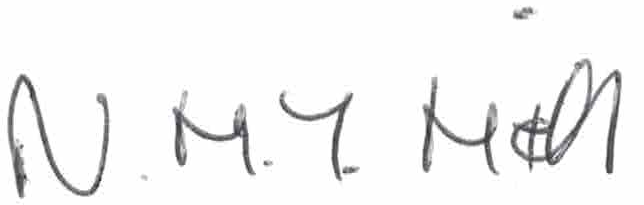
\includegraphics[scale=1]{../images/signature_real.png} %placeholder for your signature image
\newline
  \begingroup
    \setstretch{2}
    \noindent\textsf{Nicholas Hitch} \vspace{0.5cm}\\
    \noindent\textsf{\today}
  \endgroup
  \end{flushleft}

\end{enumerate}
\end{center}

\newpage

\begin{center}
\section*{Acknowledgements}
\end{center}

\noindent
Thanks to my supervisor Simon, who has provided great advice throughout allowing the report to be what it is.

\vspace{0.3cm} \noindent
Thanks to my father, Roger, who helped with proof reading, which aided in making the report more grammatically correct as well as improving readability and the flow of the report.

\vspace{0.3cm} \noindent
Lastly thanks to all the previous research that has been cited which has allowed this study to build upon  them.

\newpage

\pagenumbering{roman}
\setcounter{page}{1}
\vspace*{\fill}
\begin{center}
\begin{huge}
Intentionally Blank
\end{huge}
\end{center}
\vspace{\fill}

\newpage

\begin{center}
\section*{Executive Summary}
\end{center}
\addcontentsline{toc}{section}{Executive Summary}

\noindent
This report is one of the required modules for the course \texttt{MSc in Information Security} at Royal Holloway, University of London. A longitudinal study for the adoption of several security mechanisms, including: \texttt{Transport Layer Security}, \texttt{Content Security Policy}, \texttt{STS Preloading} and \texttt{Security.txt} is undertaken.

\vspace{0.3cm} \noindent
This is accomplished by scanning the top 1 million ranked domains each day for over 12 months from November 2020 through to the end of January 2022 and subsequent analysis of the data in order to determine the adoption of the security mechanisms.

\vspace{0.3cm} \noindent
The analysis finds that the usage of TLS versions is trending in the right direction with TLS 1.3 reaching a 64.4\% proportion of all from establishment of a TLS connection to websites in the top 1 million ranked domains.

\vspace{0.3cm} \noindent
There is still wide spread usage of the \texttt{unsafe-inline} and \texttt{unsafe-eval} keywords in Content Security Polices especially with the \texttt{script-src} directive which allows a great attack vector for cross site scripting attacks.

\vspace{0.3cm} \noindent
There are a relatively large proportion of domains that are STS preloaded but no longer meet the STS preload requirements which puts them at risk of being removed from the STS preload list.

\vspace{0.3cm} \noindent
The security.txt mechanism currently has low utilisation, however the RFC is still in the draft stage and the number of domains using this mechanism is trending upward. Even with the low usage, the number of security.txt that have a Contact is encouraging.

\vspace{0.3cm} \noindent
This study also adds some novel contributions not found during the literature research phase which are:
\begin{itemize}
	\setlength\itemsep{0.1em}
	\item Analysis of TLS versions that are supported by a website are captured (rather than just the TLS version negotiated when making a HTTPS request)
	\item Analysis of the newest Cross Origin Security headers.
\end{itemize}

\vspace{0.3cm} \noindent
It should be noted that scanning of websites commenced in November 2020, before the \textit{``Project''} module was officially started in October 2021. This was due to the need to gather at least 12 months of data before the project submission deadline at the end of March 2022.


\newpage
\begin{center}
\section*{Acronyms}
\end{center}
\addcontentsline{toc}{section}{Acronyms}

\noindent \textbf{API} Application Programming Interface \par
\vspace{0.5cm}
\noindent \textbf{CSS} Cascading Style Sheets \par
\noindent \textbf{CORS} Cross-Origin-Request-Sharing \par
\noindent \textbf{CSP} Content Security Policy \par
\vspace{0.5cm}
\noindent \textbf{DOM} Document Object Model \par
\vspace{0.5cm}
\noindent \textbf{FIPS} Federal Information Processing Standards \par
\vspace{0.5cm}
\noindent \textbf{HTML} Hypertext Markup Language \par
\noindent \textbf{HPKP} HTTP Public Key Pinning \par
\noindent \textbf{HTTP} Hypertext Transfer Protocol \par
\vspace{0.5cm}
\noindent \textbf{MIME} Multipurpose Internet Mail Extensions \par
\vspace{0.5cm}
\noindent \textbf{URI} Uniform Resource Identifier \par
\noindent \textbf{URL} Universal Resource Locator \par
\vspace{0.5cm}
\noindent \textbf{SSL} Secure Socket Layer \par
\vspace{0.5cm}
\noindent \textbf{TLS} Transport Layer Security \par
\vspace{0.5cm}
\noindent \textbf{XSS} Cross-Site Scripting \par

\newpage

\begin{center}
\section*{Glossary}
\end{center}
\addcontentsline{toc}{section}{Glossary}

\begin{hangparas}{.25in}{1}
\textbf{Application Programming Interface} is an interface intended to be used by a computer program for the purpose of allowing two computer programs to communicate to one another in a structured format. \par
\vspace{0.5cm}
\textbf{Cascading Style Sheets} is a mechanism by which a web page can be styled by many different aspects such as fonts, colours and spaces. \par
\textbf{Cipher Suite} defines the implementation of cryptographic primitives and additional information referable via a unique identifier such as \UScore{TLS_ECDHE_RSA_WITH_AES_128_GCM_SHA256} for the use in establishment of SSL/TLS connections \cite{Ristic2017-aj}. \par
\textbf{Cross Origin-Request-Sharing} is a web browser mechanism for the purpose of allowing a resource to specify the origins allowed to access the resource via the use of HTTP Headers. \par
\textbf{Cross Site Scripting} A browser attack whereby a malicious script is inserted into a web page for the purpose of performing wanted actions on a user’s online account and or gaining access to sensitive information (e.g. authentication cookies and session identifiers) usually via a web browser. \par
\textbf{Content Security Policy} is a HTTP protocol feature to restrict which resources can be fetched and or executed, such as for the purposes of obtaining content e.g. images, whilst on a specific web page in a web browser. The policy details can be specified in either a HTTP Header or in the head section of a web page via the meta tag. \par
\vspace{0.5cm}
\textbf{Document Object Model} is the web browsers internal representation of an html page as a result of the browser parsing the html \cite{Apple_undated-ay}. \par
\vspace{0.5cm}
\textbf{Federal Information Processing Standards} standards for federal computer systems which are developed by the National Institute of Standards and Technology (NIST) \par
\vspace{0.5cm}
\textbf{Hypertext Markup Language} a standardised language to create documents \cite{Berners-Lee1995-hg} for instructing a web browser how a web page should be rendered/visualised. \par
\textbf{Hypertext Transfer Protocol} a stateless application level protocol \cite{Berners-Lee1996-ji} for the transmission of data (e.g. HTML) typically between a website and a web browser. \par
\vspace{0.5cm}
\textbf{Multi-purpose Internet Mail Extensions} is used to announce the intended format of a resource (e.g document or file) \cite{Freed2013-yn}. \par
\vspace{0.5cm}
\textbf{Universal Resource Locator} a specific type of URI that has a scheme (how to access) and a resource (where to access). The most basic form of a URI is as follows \texttt{$<$scheme$>$:$<$scheme-specific-part$>$}. An example URL is \newline \texttt{https://www.example.com} \par
\vspace{0.5cm}
\textbf{Secure Socket Layer} a protocol to establish a secure communications channel mainly used by the HTTP protocol \par
\vspace{0.5cm}
\textbf{Transport Layer Security} a protocol, successor of the SSL protocol, to establish a secure communications channel mainly used by the HTTP protocol \par

\end{hangparas}
\clearpage
\newpage

\addcontentsline{toc}{section}{\listfigurename}
\listoffigures

\clearpage
\newpage
\addcontentsline{toc}{section}{\listtablename}
\listoftables

\clearpage
\newpage

%\printglossary[type=\acronymtype,title=List of Abbreviations,nonumberlist]
%\newpage




\tableofcontents

\newpage
\pagenumbering{arabic}
%\chapter*{Introduction}
\section*{Introduction}
\addcontentsline{toc}{section}{Introduction}
\label{section:intro}


\noindent
The world revolves around internet communication and websites are a big part of that. There have been many security improvements to the technology that powers the HTTPS ecosystem and as such, analysing how these are or are not being utilised is of great interest and value to the community.

\vspace{0.3cm} \noindent
Security is a battle ground with attackers ever changing their techniques and defenders doing their best to thwart the attackers attempts.

\vspace{0.3cm} \noindent
In 1994 SSL was proposed \cite{Oppliger2016-ig,Wu2016-nx} to make interactions with websites more secure. As time has moved on, more improved secure channel protocols, such as TLS 1.3 [RE01]\cite{Rescorla2018-wb} being the most recent, have been introduced as well as enhancements to HTTP through security headers such as HTTP Strict Transport Security \cite{Hodges2012-pe}.

\vspace{0.6cm} \noindent
\centerline{\texttt{What is the current adoption of security mechanisms}}
\centerline{\texttt{in the HTTPS ecosystem ?}}

\vspace{0.6cm} \noindent
It is likely that with the more complicated the security mechanism are to deploy and or implement, the less use it will see. This research intends to discover to what extent are security mechanisms currently deployed and attempt to determines possible reasons for large or small adoptions. Once the adoption has been measured it shall be compared to similar research to seek indications of adoption trends.

\clearpage
\newpage

\section*{Objectives and Scope}
\addcontentsline{toc}{section}{Objectives and Scope}

In order to conduct research to answer the question stated in the introduction in an constructive manner, one must set out a list of objectives to be completed:

\textit{
\begin{enumerate}
  \item Identify security mechanisms of which to measure the adoption.
  \item Analyse previous related measurement research for data capture methodology.
  \item Scan services in the HTTPS ecosystem to obtain the required data to be able to measure adoption of the chosen security mechanisms.
  \item Analyse the adoption of chosen security mechanisms.
  \item Compare and contrast the analysis outcomes to related research.
\end{enumerate}
}

\vspace{0.3cm} \noindent
There are many services in the HTTPS ecosystem such as websites and API interfaces and as such the target(s) of measurement will be restricted otherwise the research could take a very long time if not endless. The research will be scoped by the following criteria:

\textit{
\begin{enumerate}
  \item The measurements will be restricted to websites as they are interacted with by a large proportion of people today, thus providing useful analysis targets.
  \item Scan websites no more than once a day for a period of at least 12 months.
  \item Restrict the websites scanned to the top 1 million most popular.
  \item Only metadata, i.e. headers and connection details, will be captured and not the body content of websites.
\end{enumerate}
}

\newpage

\section*{Document Structure}
\label{section:doc_struct}
\addcontentsline{toc}{section}{Document Structure}

This report going forward is structured as follows:

\vspace{0.3cm} \noindent
\hyperref[chap:sec_feat_primer]{\textbf{Chapter \ref{chap:sec_feat_primer} - Security Mechanisms Primer}} provides a breif background of relevant technologies related to the security mechanisms to be analysed. The chosen security mechanisms to be analysed are given a brief overview along with any attacks they are designed to mitigate.

\vspace{0.3cm} \noindent
\hyperref[chap:sec_feat_exist]{\textbf{Chapter \ref{chap:sec_feat_exist} - Why Security Features Exist}} details the need for security mechanisms, focusing on those mentioned in Part I, including the following attacks: \textit{Cross Site Scripting (XSS)}, \textit{Supply Chain Attacks}, \textit{Clickjacking} and \textit{Entity in the Middle Attacks}.

\vspace{0.3cm} \noindent
\hyperref[chap:data_acqusition]{\textbf{Chapter \ref{chap:data_acqusition} - Data Acquisition}} discusses internet scanning, the issues to be aware of and how other similar research has captured their data. This part concludes with detailing how this project carried out the data capture.

\vspace{0.3cm} \noindent
\hyperref[chap:analysis]{\textbf{Chapter \ref{chap:analysis} - Security Mechanism Adoption Analysis}} analyses the chosen security mechanisms described in Part I from the data captured, over a 16 month period from November 2020 to February 2022, as detailed in Part III.

\vspace{0.3cm} \noindent
\hyperref[chap:sec_mech_overview]{\textbf{Chapter \ref{chap:sec_mech_overview} - Security Mechanisms Overview}} goes into further detail about each security mechanism that will analysed. This is to allow the reader to gain further context for the analysis chapter.


\vspace{0.3cm} \noindent
\hyperref[chap:conclusion]{\textbf{Chapter \ref{chap:conclusion} - Conclusions and Closing Remarks}} brings the report to an end concluding that apart from TLS the other chosen security mechanism that are currently not deprecated are of relatively low usage and work needs to be done to improve this.

\newpage

%\vspace*{\fill}
%\begin{center}
%\begin{huge}
%Part I - Security Features Primer
%\end{huge}
%\end{center}
%\vspace{\fill}
%
%\newpage

\chapter{Security Features Primer}
\label{chap:sec_feat_primer}

\section{HTTP}
\label{section:http}

HTTP (Hypertext Transfer Protocol), standardised in 1996 \cite{Berners-Lee1996-ji}, is a stateless protocol used for the transmission of data between a web browser and a website. When one enters an address into the address bar of a web browser or clicks a link on a web page, HTTP is used to send the request to and receive the response from a website.

\subsection{HTTP Headers}

\noindent HTTP Headers make up part of the additional meta-data that accompanies a request and response payloads on the HTTP protocol.

\vspace{0.3cm} \noindent
Headers are key value pairs delimited by the colon \texttt{:} character \cite{Berners-Lee1996-ji}. The key of a header is case insensitive.

\vspace{0.3cm} \noindent
An example header would be \texttt{server: nginx} where \texttt{server} is the key and \texttt{nginx} is the value.

\subsection{HTTP Methods}

\noindent HTTP has a number of methods for the purpose of denoting the intended request action that the request initiator is requesting to perform on a resource.

\vspace{0.3cm} \noindent
The below are relevant methods for this project:
\begin{itemize}
	\setlength\itemsep{0.1em}
	\item GET – Requests a specified resource without altering the resource.
	\item HEAD – Identical to the GET method without the resource being returned (i.e. only metadata such as HTTP Headers)
\end{itemize}

\subsection{HTTPS}

\noindent The S in HTTPS signifies that the HTTP protocol communication shall be over a secure channel, provided by the SSL/TLS protocols \cite{Rescorla2000-fs}. A URL starting with \texttt{https://} e.g. \texttt{https://example.com} signifies it will be using a SSL/TLS secure channel.

\vspace{0.3cm}
\noindent Slowly over time HTTPS has seen an ever increasing amount of adoption. There have been several incentives over the years to encourage the use of HTTPS and reduce the barrier to entry:

\begin{itemize}
	\setlength\itemsep{0.1em}
	\item Lets Encrypt provides free certificates, a prerequisite to enable HTTPS, for websites and is currently able to issue at least 200 million certificates a day as of February 2020 \cite{noauthor_undated-bi}
	\item Search engines will rank websites higher if they use HTTPS. Google uses HTTPS as a ``very lightweight signal'' \cite{noauthor_undated-im}
	\item Google Chrome and Mozilla Firefox both start to show warnings in their browsers in 2017 when users typed in passwords on a site loaded over HTTP \cite{Vyas2017-ds,Google_undated-ws}
	\item Governments and Community resources on why to use HTTPS \cite{noauthor_undated-oz,noauthor_undated-xk}
\end{itemize}

\section{Same Origin Policy}
\label{section:same_origin_policy}
\vspace{0.3cm} \noindent
Same-Origin Policy (SOP) is a critical base security mechanism of web browsers that restricts the origin of a resource (e.g. script) to only be able to communicate to resources from the same origin.

\vspace{0.3cm} \noindent
The concept of SOP started in 1996 with the release of Netscape Navigator 2.0 \cite{Preston2012-cs} and standardised by The Web Hypertext Application Technology Working Group (WHATWG) \cite{Multiple1996-ju}

\vspace{0.3cm} \noindent
If the scheme (e.g. \texttt{https://}), port (e.g. 443) and host (e.g. images.example.com) are the same for two URLs they are deemed to be in the same origin. The combination of scheme, port and host can be referred to as the origin tuple or triplet.

\vspace{0.3cm} \noindent
A request is deemed to be ``cross origin'' when the origin triplets of the url of the request being made is different from that of the origin of the request.

\vspace{0.3cm} \noindent
The path of a URL after the origin triplet is NOT evaluated when origins are being compared, for example the origin triplet of \texttt{https://example.com/index.html} is \newline \texttt{https://example.com}.

\vspace{0.3cm} \noindent
Table \ref{table:sopviolations1} shows some origin triplets via the comparison of origins to the url \newline \texttt{https://shop.example.com/index.html} which is of the origin \newline \texttt{https://shop.example.com}.

\begin{table}[h!]
%\tiny
  \begin{center}
  \resizebox{\textwidth}{!}{
    \begin{tabular}{|l|D|E|}  % <-- Alignments: 1st column left, 2nd middle and 3rd right, with vertical lines in between
      \hline
      \multicolumn{1}{|{c}|}{\textbf{URL}} & \textbf{Same Origin Triplet Violation} & \textbf{Reasoning}\\
      \hline
      https://shop.example.com/books.html & No & The difference \newline is after the origin triplet\\
      \hline
      https://shop.example.com/music.html & No & The difference is after the origin triplet\\
      \hline
      https://blog.example.com/index.html & Yes & The host of the origin triplet, blog.example.com, is different.\\
      \hline
      https://shop.example.com:8000/forum.html & Yes & The port of the origin triplet is different (HTTPS default port is 443)\\
      \hline
      http://shop.example.com/index.html & Yes & The scheme of the origin triplet, HTTP, is different.\\
      \hline
    \end{tabular}}
    \caption{Same Origin triplet example violations}
    \label{table:sopviolations1} % label MUST be after caption https://stackoverflow.com/questions/1353120/referring-to-a-table-in-latex
  \end{center}
\end{table}

\subsection{Cross Origin Network Requests}
A Cross origin request is one that is between two different origins, examples of which are shown as a violation in table \ref{table:sopviolations1}.

\vspace{0.3cm} \noindent
Cross Origin network requests can be summarised into 3 different categories:
\begin{itemize}
	\setlength\itemsep{0.1em}
	\item Cross-Origin reads are mostly denied (to prevent attacks such as XSS which is discussed further in section \ref{subsection:XSS}.
	\item Cross-Origin embedding is mostly allowed (e.g. \texttt{$<$script src="…"$><$/script$>$})
	\item Cross-Origin writes are mostly allowed (e.g. form submissions, links and redirects)
\end{itemize}

\subsection{Cross Origin Request Sharing}
\label{section:Cross-Origin-Request-Sharing}
Cross-Origin-Request-Sharing (CORS) can be used to override the default SOP behaviour, however it must be used with caution to limit exposure to attacks.

\vspace{0.3cm} \noindent
A request is deemed to be ``cross origin'' when the origin triplets of the url of the request being made is different from that of the origin of the request. For example if a script on the web page \texttt{https://shop.example.com/index.com} which has the origin \texttt{https://shop.example.com} make a request to \texttt{https://www.domain.com/login.html} which has the origin \texttt{https://www.domain.com} the two origins are different thus the request is deemed to be cross-origin.

\vspace{0.3cm} \noindent
Cross Origin Request Sharing is a web browser mechanism for the purpose of allowing a resource to specify the restrictions to be able to access a resource via one or more of the HTTP Headers \cite{Apple2006-hk} detailed in the following sections.

\vspace{0.3cm} \noindent
Under certain circumstances a 'preflight', HTTP OPTIONS call, is made to the resource in question to obtain the criteria that must be met for the desired request to be allowed to be made.

\newpage

\section{Selected Security Mechanisms}

The following security mechanisms are those that have been selected for their adoption to be analysed. They are briefly summarised here and detailed more in depth in the analysis section for ease of reference.


\subsection{SSL/TLS}
For the context of this research, SSL/TLS provides the secure channel used to send HTTP protocol traffic securely. This is more widely known as HTTPS.

\vspace{0.3cm} \noindent
SSL/TLS provides the following security services:

\begin{itemize}
	\setlength\itemsep{0.1em}
	\item Confidentiality - the protection of data such that only those who have been given authorisation can access the data
	\item Data Origin Authentication - establishes the integrity of the SSL/TLS channel data, i.e. to be able to verify the data was sent, and not altered in transit, by the corresponding party with whom the SSL/TLS channel was established with.
	\item Entity Authentication - the ability for an entity to prove their identity using mechanisms such as digital signatures.

\end{itemize}


\subsection{Security.txt}
The ``security.txt'' mechanism is to aid in informing security researchers how to disclose security issues found on systems such as a website \cite{Foudil2021-vh}.

\vspace{0.3cm} \noindent
The specification specifies a number of locations where a ``security.txt'' file should be placed thus allowing security researchers to know where to look to find disclosure/reporting information should a site support the security.txt mechanism.



\subsection{Content Security Policy}
The Content Security Policy (CSP) mechanism allows restrictions to be specified, in either a header or HTTP meta tag, in the form of a policy.

\vspace{0.3cm} \noindent
A policy can consist of a number of directives targeted at restricting the loading/executing of resources on a web page in a browser, such as only allowing scripts to be loaded from a specific list of domains.

\vspace{0.3cm} \noindent
The main attacks that are intended to be mitigated include Cross Site Scripting (XSS), data injection , packet sniffing and supply chain attacks.


\subsection{Strict Transport Security}
The \texttt{Strict-Transport Security} response header (STS) is a mechanism that instructs the browser to load the website only over HTTPS and never HTTP \cite{Hodges2012-pe}. This prevents an attacker trying to get the user to use HTTP to access the site so that the attacker could perform an entity in the middle attack allowing them to impersonate the user or just capture sensitive information to name only a few possibilities.

\vspace{0.3cm} \noindent
There is an issue with this header such that a browser can only know to load over HTTPS when the header is received. On the first visit to a website an attacker could intercept a HTTP request to the website and keep the connection HTTP and thus the user would not get the STS header. To overcome this preloading is required.


\subsection{STS Preloading}
STS Preloading is a mechanism where a browser checks to see if the requested domain is in a predefined list and if it is then the website must only be accessed over HTTPS.

\vspace{0.3cm} \noindent
The main reason for STS Preloading is to ensure the first time a user visits a website it is over HTTPS. Without preloading, should a user visit the site the first time over HTTP, an attacker could intercept the traffic and perform malicious actions such as the entity in the middle attack as described in section \ref{subsection:entity_in_the_middle}.

\vspace{0.3cm} \noindent
Google maintains this predefined list of websites where the website owners/maintainers have requested to be added \cite{Hodges2012-pe}.


\subsection{Cross Origin Resource Policy}
The Cross Origin Resource Policy is used to restrict which origins are allowed to read resource(s), such as scripts and images, protected by this mechanism.

\vspace{0.3cm} \noindent
A primary class of attacks that this mitigates against are speculative side-channel attacks. The Spectre attack \cite{Kocher2019-gv} is one such attack which was publicly announced in 2018.


\subsection{Cross Origin Embedder Policy}
The Cross Origin Resource Policy allows a website maintainer to require that any cross-origin resources are only allowed to be loaded if the resource is explicitly permitted to do so via a Cross Origin Resource Policy (CORP) or a Access Control Allow Origin CORS header or meta tag.

\vspace{0.3cm} \noindent
A driving factor for this header being introduced was that some developers may implement CORS in minimal way, such as setting the requesters origin in the Access-Control-Allow-Origin header \cite{noauthor_undated-cr}. This may have the undesired affect of allowing potentially sensitive data to be accessed unintentionally.

\vspace{0.3cm} \noindent
COEP has a lower risk than CORS of a similar situation form occurring as it is a lower privilege than CORS.


\subsection{Cross Origin Opener Policy}
The \texttt{Cross-Origin-Opener-Policy} (COOP) header provides a mechanism that prevents the sharing of browsing contexts of a top-level document with cross-origin documents. For example, preventing a popup window from communicating to the web page (document) that opened the popup via the use of process isolation \cite{Apple_undated-gj}.

\vspace{0.3cm} \noindent
This is also known as a process-isolation mechanism, preventing attackers from gaining access to a global object that created a popup window/tab for example.


\subsection{X Content Type Options}
The \texttt{X-Content-Type-Options} (XCTO) mechanism is used to enforce that the ``Multipurpose Internet Mail Extensions'' (MIME) specified in the \texttt{Content-Type} header (e.g. \newline 
\texttt{Content-Type: text/css}) matches that of the requested resource \cite{Apple_undated-hz}.

\vspace{0.3cm} \noindent
This mechanism is intended to mitigate against such attacks as \textit{drive by downloads} and untrusted user content being treated as an executable.


\subsection{X Frame Options}
The \texttt{X-Frame-Options} (XFO) response header is a mechanism that states if a browser should load the url in question in any of the following html elements: \texttt{$<$frame$>$}, \texttt{$<$iframe$>$}, \texttt{$<$embed$>$}, or \texttt{$<$object$>$}.

\vspace{0.3cm} \noindent
This mechanism is intended to mitigate against such attacks as clickjacking where an attacker invisibly embeds another site on top of theirs tricking users, via the use of enticing offers such as free electronics, into clicking a seemingly harmless link which actually triggers a function on the embedded site such as transferring money via one's banking website to the attacker.


\subsection{Public Key Pinning}
The \texttt{Public-Key-Pins} (HPKP) response header is a mechanism that permits a cryptographic public key to be advertised that must be matched to the website certificate presented during the SSL/TLS connection establishment otherwise the website will be prevented from loading/rendering.

\vspace{0.3cm} \noindent
This header was intended to protect websites in the event a CA provider was compromised, such as DigiNotar in 2011 \cite{Amann2017-co}, and unauthorised certificates being issued to an attacker for the purposes of impersonating websites. The HPKP mechanism would prevent the unauthorised certificate from being trusted by visitors that had previously visited the website i.e. preventing an entity in the middle attack.
\newpage

%\vspace*{\fill}
%\begin{center}
%\begin{huge}
%Part II - Why Security Features Exist
%\end{huge}
%\end{center}
%\vspace{\fill}
%
%\newpage

\chapter{Why Security Features Exist}
\label{chap:sec_feat_exist}

\section{The Need for Security Mechanisms}
\label{section:need_for_security_mechanisms}

As communication technologies continually improve, it has allowed and attracted an ever-increasing amount of people to interact with services on the internet. Malicious actors and security researches are drawn to this large online user base interacting with online services such as those that:
\begin{itemize}
	\setlength\itemsep{0.1em}
	\item process payments \cite{Herman2019-zb}
	\item provide online banking \cite{Gezer2019-oy}
	\item contain confidential information (e.g. medical related data) \cite{Mrdjenovich2020-vz}
	\item provide communication channels (e.g. social networks and forums)
\end{itemize}

\vspace{0.3cm} \noindent
There are many entities that track trends and malicious activity, one of which is the non-profit organisation Open Web Application Security Project (OWASP) which works to advance the security of applications \cite{noauthor_undated-ta,Kellezi2021-nd}.

\vspace{0.3cm} \noindent
OWASP maintain a Top Ten list, determined using a publicised methodology, which state the most important risks to web applications \cite{Kellezi2021-nd,noauthor_undated-kz}. In the 2021 Top Ten Report, Injection attacks (of which Cross Site Scripting (XSS) detailed in section \ref{subsection:XSS} is one variant) was ranked number three and of the 94\% of the applications they tested there was an average incident rate of 3\% and 274k occurrences \cite{noauthor_undated-gt}.

\vspace{0.3cm} \noindent
The ``Global Data At Risk State of the Web'' 2020 report \cite{Tala_Security2020-ee} claims that on average, the top 1000 websites in the Alexa top one million website list, rely upon the 32 third party integrations. This gives a great opportunity for attackers to leverage the supply chain attack (detailed in section \ref{subsection:SupplyChain}) to compromise websites that may be harder to compromise directly. One such example of this attack is the 2018 Magecart attack on Ticketmaster \cite{Herman2019-zb} to steal payment information via the compromise of third party resources.

\vspace{0.3cm} \noindent
Due to the susceptibility of data traversing the internet being intercepted and attacked, its integrity and confidentially needs to be protected. For browser traffic this is achieved by the use of HTTPS, which uses SSL/TLS secure channels, instead of the insure HTTP. Unfortunately not all websites use HTTPS and or redirect to the HTTPS version should it exist. Governments are encouraging the use of HTTPS \cite{noauthor_undated-oz} as well as the community itself \cite{noauthor_undated-xk}. The general advice is that if one is in control of a website, it should be using HTTPS regardless of the websites purpose or content. 

\vspace{0.3cm} \noindent
The following attacks are ones that can be mitigated by one or more of the security mechanisms described in the previous sections of this report.

\subsection{Cross Site Scripting (XSS)}
\label{subsection:XSS}

Cross Site Scripting (XSS) attacks are part of the injection class of attacks where one or more malicious scripts, commonly written in JavaScript, are injected and subsequently executed on a web browser. There are four main variants of XSS attacks:

\subsubsection{Attack Variants}
\textbf{Reflected}

\vspace{0.2cm} \noindent
Stored XSS (also referred to as \textit{Non-Persistent}, \textit{Indirect} and \textit{Type II}) occurs as a result of when a request is made to a web application, that contains malicious content, the response contains a malicious script that is executed by the web browser. The malicious script is reflected back to the user, hence the name of this variant \cite{Rodriguez2020-bg}.

\vspace{0.6cm} \noindent
\textbf{Stored}

\vspace{0.2cm} \noindent
Stored XSS (also referred to as \textit{Persistent}, \textit{Direct} and \textit{Type I}) is where a malicious actor is able to store a malicious script on a website, by some means such as a forum post or comment section of a website such that the script will be executed, by the web application when a victim visits the page. The power of this variant is that the script is permanent, until when or even if the script is detected and removed. This variant has the potential to have many visitors to become victims depending of the traffic of the compromised web page(s) \cite{Rodriguez2020-bg}.

\vspace{0.6cm} \noindent
\textbf{DOM-Based}

\vspace{0.2cm} \noindent
DOM-Based XSS (also referred to as \textit{Type 0}) takes place entirely in the DOM. The Document Object Model (DOM) is the web browsers internal representation of an html page as a result of the browser parsing the html. The source (e.g. the parsed html), functionality and destination of the malicious script is all contained within the DOM \cite{Rodriguez2020-bg,Klein2005-hx}.

\vspace{0.6cm} \noindent
\textbf{Mutation Based}

\vspace{0.2cm} \noindent
Mutation Based XSS (also referred to as \textit{mXSS}) is based on the use of the \texttt{innterHTML} functionality, often used to provide web application users to do custom styling, of a browser which allows direct manipulation of the HTML content bypassing the DOM entirely. The malicious actor crafts a ``mutated'' payload that once processed by the \texttt{innerHTML} functionality allows the script to execute \cite{Heiderich2013-qv}.

\subsubsection{Historical Example}
In October of 2005 it was discovered that when users visited an infected MySpace profile the phrase ``but most of all, samy is my hero'' was appended to the ``hero'' section of visiting users profiles. The infected profile contained a stored XSS payload which added itself to the visiting users profile and adding the aforementioned phrase. The attack was initiated by ``Samy'' infecting his own profile with the XSS payload. Over one million user profiles were reported to have been affected within 20 hours \cite{Lee2019-xf}.

\vspace{0.2cm} \noindent
The attack is known as the ``Samy Worm'' as it propagated to other MySspace profiles just by visiting an infected profile.

\subsubsection{Security Mechanism(s) Providing Mitigation}

\begin{itemize}
	\setlength\itemsep{0.1em}
	\item Content Security Policy (CSP) – multiple directives
	\item Cross-Origin-Resource-Policy
	\item X-Frame-Options
\end{itemize}


\subsection{Supply Chain}
\label{subsection:SupplyChain}

Supply chain attacks are when a malicious entity maliciously alters one or more third party resource(s) (such as a JavaScript library) that a web application uses, commonly hosted on a third party location such as a CDN. These malicious modifications are for several reasons including:

\begin{itemize}
	\setlength\itemsep{0.1em}
	\item Running a cryptominer \cite{Tekiner2021-sq} on browsers
	\item Capturing Payment Information
	\item Screen Scraping
	\item Ad injection
\end{itemize}

\subsubsection{Historical Example}
The 2018 Texthelp breach is one example of this type of attack where a malicious entity compromised a JavaScript library and modified it to include a cryptominer. A cryptominer uses computing resources to mine cryptocurrency such as (Bitcoin, Etherium and Monero). This single compromised JavaScript library was reportedly found to be used on 4,000 websites \cite{Billman2018-sq}.

\subsubsection{Security Mechanism(s) Providing Mitigation}

\begin{itemize}
	\setlength\itemsep{0.1em}
	\item Content Security Policy (CSP) - sub resource integrity
\end{itemize}

\subsection{Clickjacking}

A clickjacking attack is one in which a user-initiated attack is hijacked to perform unwanted actions. A user is enticed to click on an element of a page, such as an image, however rather than an action or outcome the user expects to occur, one determined by the attacker takes place. To undertake the attack a malicious site renders a web page from the target website within an iframe. The malicious site uses styling to show only what the attack desires of the target website \cite{Jamwal2018-tz}.

\subsubsection{Historical Example}
The Twitter Attack, also referred to as the ``Twitter Bomb'', begins by a user seeing a twitter post that contains the text \texttt{Don't Click: http://tinyurl.com/amgzs6} \cite{Jani2015-kw} and clicking on the link. Visiting the link will present the user with a page seemingly only containing only a single button ladled \texttt{Don't Click}.

\vspace{0.3cm} \noindent
Unbeknownst to the user, the twitter home page is also rendered on the page but in an invisible iframe. The \texttt{Don't Click} button is directly underneath the invisible ``update'' button, which posts a tweet of the twitter home page. The iframe is configure to load the url \texttt{http://www.twitter.com/?status=Don't Click: http://tinyurl.com/amgzs6} \cite{Jani2015-kw} and twitters \texttt{?status=} feature will pre-load the users tweet box with the status message.

\vspace{0.3cm} \noindent
When the user clicks the \texttt{Don't Click} section of the page they are actually clicking the invisible \texttt{update} button of the twitter home page which creates a tweet with the text \texttt{Don’t Click: http://tinyurl.com/amgzs6} \cite{Jani2015-kw} which helps to spread the message. There was no ill intent to this clickjacking attack and as such considered more of a prank.
\subsubsection{Security Mechanism(s) Providing Mitigation}

\begin{itemize}
	\setlength\itemsep{0.1em}
	\item Content Security Policy (CSP) – frame-ancestors directive
	\item X-Frame-Options
\end{itemize}

\subsection{Entity in the Middle}
\label{subsection:entity_in_the_middle}

Malicious actors are constantly on the lookout for ways to obtain sensitive data for a multitude of reasons including: intellectual property theft, stealing money and personal information.

\vspace{0.3cm} \noindent
One of the ways to help prevent this is to secure the communication traffic over the internet using HTTPS which relies on the SSL/TLS mechanism.

\vspace{0.3cm} \noindent
If a malicious actor is able to intercept and or passively monitor web traffic, the opportunity arises to perform what is known as an Entity in the Middle attack.

\vspace{0.3cm} \noindent
The Entity in the Middle attack is where an attacker is able to intercept and manipulate traffic between the victim and the target entity such as a website. This can lead to attacks such as victims unknowingly giving their credentials to attackers as well as attackers manipulating the response from the website before being sent back to the victim.

\vspace{0.3cm} \noindent
Over the years there have been several attacks against the SSL/TLS mechanism, compromising the confidentiality and or integrity of the information it is meant to secure.

\subsubsection{Historical Examples}
\textbf{BEAST (2011)}

\vspace{0.2cm} \noindent
The BEAST attack, announced in 2011, was for use against TLS 1.0. The attack exploited the TLS 1.0 implementation of the Cipher Block Chaining (CBC) encryption mode in order to be able to decrypt parts of TLS 1.0 data packets to reveal sensitive data such as website cookies that could be used to impersonate a user on a web application \cite{Ristic2017-aj,Levillain2015-os}. Modification of padding, the primary exploitation vector, used in this attack is referred to by the term ``padding oracle''. The vulnerability was fixed in TLS 1.1.


\vspace{0.6cm} \noindent
\textbf{Lucky 13 (2013)}


\vspace{0.2cm} \noindent
The Lucky 13 attack is where a malicious attacker modifies, in transit, the padding (redundant data to make the data packet a certain size) of TLS data packets, that are using a CBC cipher suite, to analyse how the server reacts. Should the malicious actor be able to determine that the server has reacted to the modifications of padding, then this can lead to information leakage and plain text recovery \cite{Ristic2017-aj,Al_Fardan2013-sw}. This attack is effective against TLS 1.0 - 1.3 and SSL 3.0 that use CBC mode (or any other mode that do not have padding oracle countermeasures.)


\vspace{0.6cm} \noindent
\textbf{Poodle (2014)}

\vspace{0.2cm} \noindent
The Poodle attack is similar to the Lucky 13 attack, where unprotected padding is exploited, but restricted to SSL 3.0. In order to force the use of SSL 3.0 the malicious attacker performed a downgrade attack which prevented a TLS handshake for any protocol version higher than SSL 3.0 to be established \cite{Ristic2017-aj,Al_Fardan2013-sw}. The downgrade attack was possible as servers would fall back to SSL 3.0 should higher protocol versions fail.


\vspace{0.6cm} \noindent
\textbf{Heartbleed (2014)}

\vspace{0.2cm} \noindent
The 2014 Heartbleed attack, which gained attention in the mainstream media, exploited an implantation flaw in the length of a data bounds check. The flaw was in the rarely used but commonly enabled heartbeat protocol \cite{Durumeric2014-yj} of the TLS mechanism in the OpenSSL library (used by millions of servers).

\vspace{0.2cm} \noindent
To exploit the vulnerability, a malicious actor would send a \texttt{HeartbeatRequest} message, setting the payload length set to a length larger than the actual \texttt{HeartbeatRequest} message payload length \cite{Durumeric2014-yj}. This allowed the extraction of private memory on the target which could lead to the ex-filtration of sensitive data such as website private keys and cryptographic secrets.

\vspace{0.3cm} \noindent
The maintainers of the OpenSSL library released a fix for the vulnerability alongside the public announcement of the vulnerability \cite{Durumeric2014-yj}.


\vspace{0.6cm} \noindent
\textbf{FREAK (2015)}

\vspace{0.2cm} \noindent
The 2015 FREAK attack shed light that the OpenSSL library would accept weak RSA encryption keys, from the use of export grade cipher suites, during a full-strength RSA TLS handshake. A malicious actor would force the client to use such a weak key by sending a \texttt{SeverKeyExchange} TLS protocol message to the client. If such a weak key was used the malicious actor could capture the traffic, brute force the key within a matter of hours and decrypt the captured traffic. The removal of export grade cipher suites on the server stops this attack \cite{Ristic2017-aj,Beurdouche2015-ga}.

\subsubsection{Security Mechanism(s) Providing Mitigation}

\begin{itemize}
	\setlength\itemsep{0.1em}
	\item TLS/SSL
	\item Strict Transport Security
	\item STS Preloading
	\item Public Key Pinning
\end{itemize}

Organisations should have policies in place to keep up to date with current state of TLS vulnerabilities and best practice recommendations to best mitigate risk to themselves and their users from malicious actors.
\clearpage
\newpage

%\vspace*{\fill}
%\begin{center}
%\begin{huge}
%Part III - Data Acquisition
%\end{huge}
%\end{center}
%\vspace{\fill}
%
%\newpage



\chapter{Data Acquisition}
\label{chap:data_acqusition}


\section{Ethical Considerations}
\label{section:ethics}

It is not feasible to request permission to conduct internet measurement scans from the desired targets. This means that researches should take it upon themselves to evaluate their methodology for ethical considerations in the absence of permission to conduct such research.

\vspace{0.3cm} \noindent
The ethical considerations as outlined in \cite{Amann2017-co,Partridge2016-ph,Durumeric2015-zq,Kumar2017-qw} were considered for this research.

\vspace{0.3cm} \noindent
During the literature research, not all research that was of a similar nature contained ethical consideration statements. One would hope that ethic consideration was performed in the research, but should be outlined if only minimally.

\vspace{0.3cm} \noindent
The ``BCS, The Chartered Institute For It'' code of conduct \cite{Bcs2011-rj} outlines professional standards that should be met. This research was conducted with the same sentiment of these standards. Below are several of the most relevant excerpts taken from the document as presented below verbitem that represent to conduct of this research:
\begin{itemize}
	\setlength\itemsep{0.1em}
	\item \textit{``NOT disclose or authorise to be disclosed, or use for personal gain or to benefit a third party, confidential information except with the permission of your Relevant Authority, or as required by Legislation.''}
	\item \textit{``accept your personal duty to uphold the reputation of the profession and not take''
any action which could bring the profession into disrepute.}
	\item \textit{``only undertake to do work or provide a service that is within your professional
competence''}
	\item \textit{``have due regard for public health, privacy, security and wellbeing of others and
the environment''}
\end{itemize}

\subsection{Service Degradation}

Using the ``Tranco List'' which is a ``most popular'' type of domain list reduces the chance of service degradation as the more popular a domain is the more resources it is likely has which reduces the impact of the measurement analysis.

\vspace{0.3cm} \noindent
For the purpose of obtaining the HTTP headers of a domain the ``Home Page'' of the domains are requested which are more likely to be cached than other pages.

\vspace{0.3cm} \noindent
To determine the TLS versions supported by a domain, other than that used on the HTTPS request to the home page, pure TLS connections are attempted which reduces the service impact as HTTP requests will add additional load to that of pure TLS connections. Additionally pure TLS connections are only attempted if an HTTPS connection was successful to a domain's home page.

\vspace{0.3cm} \noindent
Whilst obtaining the STS preload state of a domain, as detailed in section \ref{subsection:stage_5_STS}, it is first checked if a url has already been requested. During the processing of a task, including redirects, it is quite possible that the information sought has already been obtained.

\vspace{0.3cm} \noindent
There is no retry logic for a request to a domain to additionally reduce service degradation of the target domain.

\vspace{0.3cm} \noindent
Randomisation is another potential tactic, however as the research uses a domain list rather than ip addresses. For randomisation to be effective the ip addresses would need to be pre resolved which is not being undertaken in this research.

\subsection{Exploitation}

The software used to conduct the research against domains does not attempt to:

\begin{itemize}
	\setlength\itemsep{0.1em}
    \item Send malformed requests
    \item Login
    \item Exploit vulnerabilities
    \item Access hidden/private paths/URLs
\end{itemize}

\subsection{Information Disclosure}

As this research obtains publicly available information and is not revealing vulnerabilities about any particular domain, there is not a concern of exposing information about domains that may reveal vulnerabilities.

\subsection{Abuse Reports}

As the domains being scanned have not given permission for research to be conducted upon them, the ip addresses that conduct the research have rDNS (reverse DNS) entries configured such that complaints/enquires can be submitted.

\vspace{0.3cm} \noindent
The cloud service providers for the servers that conduct the research have easy to use interfaces to allow responses to abuse reports should they be submitted.

\vspace{0.3cm} \noindent
The software that conducts the research was pre-equipped with a deny list for both ip addresses and domains. Both ip addresses and domains are required as an IP address can host more than one domain and a complaint may ask to block an IP address range.

\vspace{0.3cm} \noindent
There was a single abuse report, which came from the Cybersecurity and Infrastructure Security Agency (CISA) \cite{noauthor_undated-fh} USA government agency, which stated a request for ``assistance in verifying possible malicious activity being hosted on a system registered to you''. The reported domain and time of request was checked and the task agent made the request to the domain at the time the abuse report stated. A response to the report was made stating that the request was made for the purpose of internet research.

\newpage


\section{Data Acquisition}
\label{section:data_aquisition}

In order to be able to analyse HTTP Security Headers, TLS Versions, STS Preloading and security.txt adoption, or lack thereof, data on these desired metrics needs to be acquired. There are several overarching ways to acquire the desired data: Active, Passive and Third-Party data sets.

\vspace{0.3cm} \noindent
Active data collection is the act of establishing TLS connections and or making HTTP requests and storing the resultant connection/request/response data. This method requires the setup of infrastructure and software, which can involve the customisation and or development of entire software applications. Active scanning gives great versatility, however care needs to be taken to ensure the data is collected in a methodical and ideally a reportable way, in order for the analysis to have meaning.

\vspace{0.3cm} \noindent
Passive data collection is capturing data as it flows through network infrastructure. The infrastructure required is likely to be less than that of active collection as it should only require the duplication of pre-existing network traffic to a device that is able to store the data. With any sort of data collection there is the always the ethical consideration to take into account, however with passive collection privacy is of higher concern than active data collection and needs to be treated as such.

\vspace{0.3cm} \noindent
Third Party data sets is the use of data collected by another entity that is using passive and or active collection. The only infrastructure that should be needed by the researcher would be that needed to analyse the data. There is great trust that the third party has conducted the data collection in a way that makes the analysis of it meaningful.

\subsection{Scanning Targets}
Active data collection, for the purpose of measuring security mechanism adoption, requires a list of entities to collect data from. Generating a list of domains to scan on ones own could be potentially quite an arduous task. Using resources that contain collections of domains is a much easier task, assuming the collection is of high relevance to the research that is to be conducted.

\subsubsection{Pre-complied Lists}

Pre-compiled, often ranked by popularity, domain lists are made available by organisations that claim they are in a position to create such lists such as: Alexa Top 1 Million sites \cite{noauthor_undated-wh}, Cisco Umbrella \cite{noauthor_undated-ku}, Majestic Million \cite{noauthor_undated-sz} and Tranco \cite{noauthor_undated-mt}. These lists are updated regularly, as often as once a day, which allows researchers to have up to date lists that are freely available.

\vspace{0.3cm} \noindent
The Alexa Top 1 Million site is a favourite among researchers as shown by use in \cite{Buchanan2018-xz,Chen2016-dl,Kumar2017-qw,Patil2017-bg,Ying2016-ag,Michael2015-hn,Van_Goethem2014-ao,Holz2020-ha,Poteat2021-zr}. These lists are primarily used as they are intended to reflect the most popular sites on the internet and thus are assumed to be ones that would use the most up to date security mechanisms.

\subsubsection{Zone Lists}

Zone Lists, such as a country code top level domain (ccTLD) zone lists, which is a list of domains for a country, are another source of domains to scan. These are generally used when the researcher's intent is to gain insight into an entire country or continent such as the EU \cite{Amann2017-co,Chen2016-dl,Van_Goethem2014-ao,Holz2020-ha}.

\vspace{0.3cm} \noindent
The majority of zone lists are not openly available however ICANN has created the ``Centralised Zone Data Service'' (CZDS) \cite{noauthor_undated-mm} which allows one to register and request access to Zone Files.

\vspace{0.3cm} \noindent
The number of domains to scan using zone lists can be in the 10s or even 100s of millions of domains which would likely require more infrastructure to scan on a regular basis compared to the use of pre-compiled lists.

\subsubsection{Search Engines}

Utilising search engines can allow additional URLs for a domain to be acquired to allow for further insight how responses might change depending on which web page of a domain is requested \cite{Chen2016-dl}.

\subsubsection{IPv4 Address Space}

Scanning the entire IPv4 Address space (i.e. all internet  IPv4 addresses) is also a source of entities to scan \cite{Kotzias2018-wd}. The major difference is the use of an IP address rather than a domain which needs to take into account that servers may respond differently if an IP address is used as the website address rather than a domain name (e.g. \texttt{https://1.2.3.4} vs \texttt{https://example.com}).

\vspace{0.3cm} \noindent
The number of internet routable IP Addresses, i.e. ip addresses that can be access over the internet, is around \(2^{32}\) total possible addresses minus approximately 288 million non route-able addresses which results in approximately 4 billion addresses.

\vspace{0.3cm} \noindent
Scanning the entire IP address range can lead to abuse reports, however these can often be revoked if the researcher works with the operator who raised the complaint to conduct the scan in a manner in which the operator deems acceptable.

\subsection{Scanning}


\subsubsection{Scanner Technologies}

\noindent
There are quite a number of scanning technologies used in measurement research and as such there does not seem to be a proffered technology overall but what the researcher(s) are comfortable with. This does makes sense in regards to if a particular technology has worked for researcher in a previous study then using it in a future study, where applicable, as they are familiar with its capabilities giving more time for other activities.

\vspace{0.3cm} \noindent
Table \ref{table:measurement_technologies} details a number of measurement technologies found to be used in previous measure during the literature research.

\clearpage
\newpage

\begin{table}[H]
\footnotesize
  \begin{center}
    \begin{tabular}{|l|E|E|}  % <-- Alignments: 1st column left, 2nd middle and 3rd right, with vertical lines in between
      \hline
      \textbf{Technology} & \textbf{Description} & \textbf{Use Case} \\
      \hline
      PHP with Curl \cite{Buchanan2018-xz} & PHP is a web programming language. Curl provides a client library for communicating to web services such as HTTP web servers & Make HTTP calls to websites and capture the response body and metadata \\
      \hline
      Goscanner \cite{Amann2017-co} & Tool for large scale TLS and SSH scans & Obtain TLS connection information ip addresses / domains \\
      \hline
      Bro \cite{Amann2017-co,Kotzias2018-wd} & A network security monitor & Passive network packet capture for TLS connection analysis \\
      \hline
      PhantomJS \cite{Chen2016-dl,Van_Goethem2014-ao} & A headless scriptable browser & A browser that can be easily used by scripts for obtaining body of website with JavaScript execution \\
      \hline
      Chrome \cite{Kumar2017-qw} & A modern desktop website browser & In headless mode, can be used to capture a page rendered as an ender user would see it \\
      \hline
      Scrapy \cite{Patil2017-bg} & A scriptable tool for extracting data from websites & Extract HTTP headers from response to a request made to a website \\
      \hline
      Java with Apache \cite{Ying2016-ag} & Java is a programming language, Apache provides a HTTP client for Java & Make HTTP calls to websites and capture the response body and metadata \\
      \hline
      Zmap / Zgrab \cite{Michael2015-hn,Holz2020-ha,Kotzias2018-wd} & Zmap is a single packet network scanner. ZGrab is an application layer scanner. & Zmap can be used to identify IP address with open ports. ZGrab could then be use to capture the body and metadata from HTTP requests to the open port(s). \\
      \hline
    \end{tabular}
    \caption{Technologies used in previous measurement studies}
    \label{table:measurement_technologies} % label MUST be after caption https://stackoverflow.com/questions/1353120/referring-to-a-table-in-latex
  \end{center}
\end{table}

\subsubsection{Domain Resolving}

When a HTTP client makes a request to a URL (e.g. http://example.com) the client needs to lookup the IP address of the domain (e.g. example.com) in order to send the HTTP request.

\vspace{0.3cm} \noindent
Scanning a large number of domains can potentially put a strain on the DNS server the client is using to resolve the domain to an IP address. If there are a sufficiently large number of domains to be resolved at the same time, or over a very short period of time (e.g. a few seconds) it is possible that the DNS resolution will fail when there is an IP address that cannot be resolved. There are several ways around this such as pre determining the IP address for the domain \cite{Amann2017-co}, using more than DNS server and using retries.

\vspace{0.3cm} \noindent
Pre-computing DNS resolutions makes more sense when not following HTTP redirects such as for the TLS connection establishment in \cite{Amann2017-co,Holz2020-ha}.

\subsubsection{Using the WWW subdomain}

When using lists that contain base domains (e.g. example.com) it is not known if the website is actually hosted or available from the base domain. Websites are generally available from the base domain (e.g. example.com) and or its www subdomain (e.g. www.example.com).

\vspace{0.3cm} \noindent
To give a good chance of being able to obtain a HTTP response from a domain, it is common to try both the base domain and the www subdomain \cite{Chen2016-dl,Kumar2017-qw,Ying2016-ag,Michael2015-hn}. Some researchers choose not to also try the www subdomain such as in \cite{Buchanan2018-xz,Amann2017-co} (but do not necessarily state why they chose not to do so), which can lead to unnecessarily reduced data for analysis.

\subsubsection{HTTP Method}
In order to obtain HTTP Security Headers, one needs to make an HTTP Request. There are several types of HTTP Request, GET and HEAD being two of them.

\vspace{0.3cm} \noindent
HTTP HEAD requests result in only metadata being returned (this includes HTTP Headers) by the server. The main reason researchers choose to use HEAD HTTP Requests \cite{Amann2017-co} is to save compute resources on the server (as the server does not have to generate the response payload such as a html web page) as well as reducing the amount of data being sent over the network.

\vspace{0.3cm} \noindent
Whilst using HEAD requests does save server resources, which helps in the ethics of internet research of this kind, browsers perform GET requests which could potentially respond with different headers for the same URL. If the researcher is intending on analysing the response payload from a website then GET requests \cite{Chen2016-dl,Kumar2017-qw} are required.

\vspace{0.3cm} \noindent
Certain applications and programming languages, such as go \cite{noauthor_undated-lc}, allow the use of GET request without requesting the actual payload from the server which leaves just the computing resource to generate the payload. If the home page is requested this is more likely to be cached, as it will be one of the most visited pages, than other pages which also help to reduce the compute load on the target resource (e.g. website).

\subsubsection{HTTP Client Headers}

When browsers make HTTP requests to websites, they send several HTTP headers with the request. One of these headers is named \texttt{user-agent} and is often used to detect if the client making the request is a browser. When a website detects that a non-browser is making the request it can change the response which could skew the results of research such as analysing HTTP security header adoption for web browsers.

\vspace{0.3cm} \noindent
For the purposes of internet research when attempting to gather data from responses to HTTP requests that would normally be sent to a browser, the use of a browser user-agent is typically used \cite{Buchanan2018-xz, Patil2017-bg,Ying2016-ag,Lavrenovs2018-dl,Poteat2021-zr}. The declaration from researchers of the value for such headers is not always present \cite{Amann2017-co} which could leave readers potentially questioning the reliability of the resultant analysis.

\subsubsection{Redirects}

When a HTTP request is made, the HTTP protocol has the ability to redirect to a different url. This is quite normal for websites to do this and there are numerous reasons to do so, such as redirecting from the base domain e.g. (http://example.com) to the www subdomain e.g. (http://www.example.com) where the website is actually hosted. It is generally good practice to follow redirects as this is what browsers do, unless researchers wish to only analyse a response from a specific url such as the base domain in \cite{Amann2017-co}.

\vspace{0.3cm} \noindent
Researchers need to be mindful however that redirects can lead to the same resultant domain for different initial domains (e.g. http://example.com and http://mydomain.com could both redirect to http://anotherdomain.com).

\vspace{0.3cm} \noindent
This phenomenon can potentially skew analysis results if the researchers do not actively take this into account such as duplicate resultant URLs being removed as was done in \cite{Lavrenovs2018-dl}.

\subsubsection{SSL/TLS Certificate Validation}

When a TLS connection is being established a browser will try and verify the claimed identity of the website (e.g. example.com). If the server does not present all the necessary intermediate certificates, in order to be able to validate the websites claimed identity, the TLS connection will fail unless the browser already has the intermediate certificate available.

\vspace{0.3cm} \noindent
Intermediate certificates can be obtained from such means as: the website being visited, the certificate was obtained from a previously visited website, via Authority Information Access (AIA) \cite{Cooper2008-yr} or from preloading \cite{Keeler2020-yj}. For further details on PKI, including certificates and identity verification, please see \cite{Clark2013-sh,Holz2011-yv}.

\vspace{0.3cm} \noindent
It is quite common to use non browser clients to conduct research. These clients are not guaranteed to use any of the above mentioned methods for obtaining intermediate certificates not provided by a website in order to validate the websites' claimed identity. To counteract this issue, the TLS/SSL validation can be disabled for the scanning of the website and done as an offline step which enables any missing certificates to be obtained at the researcher's leisure.

\vspace{0.3cm} \noindent
It is not evident that any of the papers in the literature research conducted for this project used such an approach, possibly assuming that the number of websites that would have this issue would be minimal enough not to affect the results analysis conducted or not aware of the issue itself.

\subsubsection{Pre-Analysis Filtering}
It is generally best to collect the rawest form of data for to give the greatest possible freedom and options when conducting any analysis. If the filtering was carried out at the data acquisition phase this could restrict further analysis or potentially cause intended analysis not to be possible due to the way the data was filtered.

\vspace{0.3cm} \noindent
A potential example of this is where in \cite{Buchanan2018-xz} the researches decided to parse the headers of a HTTP response during the data acquisition phase. HTTP headers are caseless \cite{Berners-Lee1996-ji} and depending on how the filtering is done, some headers could have been missed, however if all the headers were captured this could have been a non issue during analysis.

\subsection{Scanning Frequency}

The number of times data gathered and how far apart they are, in terms of time, are important in terms of showing any potential trends and having enough data to confidently make statements from the analysis of such data.

\vspace{0.3cm} \noindent
Of the research sources that were reviewed for this project, those that conducted active scanning activities make at least two scans such as \cite{Buchanan2018-xz,Amann2017-co,Chen2016-dl,Kumar2017-qw} and some with daily scans for years \cite{Holz2020-ha}. This is discussed shortly in the literature review in section \ref{section:lit_review}.

\vspace{0.3cm} \noindent
The more data that is gathered in the same way, the higher value that analysis obtains, assuming that the methodology of the acquisition is sound.

\subsection{Monitoring}

Conducting long running data acquisition would greatly benefit from, at minimum, some basic metrics that show that a data acquisition has started, completed and if a critical issue was encountered. This would help to ensure that data acquisition was successful and to alert if not, so that it could be investigated and rectified to reduce any potential issues to the research being conducted.

\vspace{0.3cm} \noindent
The researchers in \cite{Poteat2021-zr} stated that they had a ``measurement outage'' however they do not go into detail. It is possible that monitoring could have helped to reduce and or mitigate the outage.

\subsection{Detailed Methodologies}

The majority of research reviewed for this project state the technologies used and the high level description of the methodology used to acquire the data later analysed, such as in \cite{Amann2017-co,Chen2016-dl,Van_Goethem2014-ao}.

\vspace{0.3cm} \noindent
Whilst this is generally enough for the reader to understand the high-level methodology, those who wish or are conducting similar or related research could benefit form a more detailed and formal method. There are several strategies presently available for researchers to utilise.

\vspace{0.3cm} \noindent
``Strategies for Sound Internet Measurement'' \cite{Paxson2004-hq} is one such paper with specific relevance to measurement research which is very relevant to the research for this report. The paper outlines the inherent difficulties and pitfalls one can encounter focusing on: \textit{Precision}, \textit{Meta-data}, \textit{Accuracy}, \textit{Misconception}, \textit{Calibration}, \textit{Data Volume} and  \textit{Reproduceability}.



\subsection{Literature Review}
\label{section:lit_review}

Table \ref{table:data_acquisition_lit_review} is a critical review of limitations identified in the literature research and how this project aims to address them.

\begin{center}

\footnotesize
\begin{longtable}{|C|E|H|H|}

    \caption{Data Acquisition Literature Review} 
    \label{table:data_acquisition_lit_review} \\ % label MUST be after caption https://stackoverflow.com/questions/1353120/referring-to-a-table-in-latex 
\hline
\textbf{Section} & \textbf{Limitation} & \textbf{Example(s)} & \textbf{How Addressed In This Project} \\
\hline
\endfirsthead
\multicolumn{4}{c}%
{\tablename\ \thetable\ -- \textit{Continued from previous page}} \\
\hline
\textbf{Section} & \textbf{Limitation} & \textbf{Example(s)} & \textbf{How Addressed In This Project} \\
\hline
\endhead
\hline \multicolumn{4}{r}{\textit{Continued on next page}} \\
\endfoot
\hline
\endlastfoot
      \textbf{Data Filtering} & If data is filtered during data capture, it could result in unintended data being filtered & The researches in \cite{Buchanan2018-xz} filter headers during data capture, which if not done perfectly (e.g. spelling and case) could produce unintended results. & All HTTP headers, TLS certificates/connection information is captured unfiltered\\
      \hline
      \textbf{www subdomain} & If using only the base domains for HTTP(s) requests could produce inaccurate results as not all domains serve HTTP on the base domain. The www subdomain is the most common domain to serve HTTP requests besides the base domain. & Researchers \cite{Buchanan2018-xz,Amann2017-co} do not state if the www subdomain was explicitly added during scanning. & The www subdomain is used if base domain does not have a DNS A record. \\
      \hline
      \textbf{HTTP method} & Browsers use the HTTP GET method to obtain web pages. A website might behave differently if a non GET HTTP method (e.g. HEAD) was used. Some websites may not even allow the HTTP HEAD method. & Researchers \cite{Amann2017-co} specifically use the HEAD HTTP method to reduce load on target domains. & The HTTP GET method is used which is what browsers use.\\
      \hline
      \textbf{Client Headers} & Browsers send standard request headers on the requests to a websites home page. Including as many of these headers as possible when scanning domains, allows greater browser emulation. It is quite common when a non browser user agent header is detected a different response is sent from the website. & \cite{Patil2017-bg} uses 3 user-agents, \cite{Buchanan2018-xz,Amann2017-co,Kotzias2018-wd,Poteat2021-zr,Van_Goethem2014-ao,Chen2016-dl,Kumar2017-qw,Michael2015-hn} use a single user agent. No other request headers are specified in the research. & Use chrome user agent along with other request headers as detailed in table \ref{table:task_paramters_headers}. \\
      \hline
      \textbf{SSL/TLS Verification} & If SSL/TLS verification is done at capture time there is a possibility that the client/OS does not necessarily have access to all of the Root/Intermediate certificates that a browser would have. & None of the research \cite{Patil2017-bg,Buchanan2018-xz,Amann2017-co,Kotzias2018-wd,Poteat2021-zr,Roth2020-hg,Van_Goethem2014-ao,Chen2016-dl,Kumar2017-qw,Calzavara2018-xv,Holz2020-ha,Michael2015-hn,} processes SSL/TLS verification at the analysis stage. There could be many reasons for this such as it not being common knowledge of how browsers cache certificates and or assumed to be not enough sites affected. & SSL/TLS verification is performed at the analysis phase. \\
      \hline
      \textbf{Monitoring} & When a scanning session is conducted and not monitored, one or more sessions could fail without the researcher(s) being aware for an unknown amount of time. & It is possible that the outage mentioned in \cite{Poteat2021-zr} could have been avoided or minimised by the use of effective monitoring. & Metrics of the status of scanning are created and alerted upon and investigated. \\
%      \hline
%      \textbf{Scan frequency} & The more data the better & - & - \\
      \hline
      \textbf{Scanner Tool Verification} & One cannot assume that the technology used to perform the scanning is doing what one expects or intends without due diligence being performed. & None of the research specifically calls out testing of the scanner with manual verification of results. & Successfully and unsuccessfully scanned domains were picked at random during the creation of the scanner, manually verifying results and correcting/updating scanner as required. \\
      \hline
      \textbf{Scanner Tool Flow} & The use of graphical flows allows greater accuracy for research replication and understanding. & Whilst most research gives a written overview of scanner methodology \cite{Buchanan2018-xz,Amann2017-co,Patil2017-bg,Kotzias2018-wd,Poteat2021-zr,Van_Goethem2014-ao,Chen2016-dl,Kumar2017-qw,Holz2020-ha,Michael2015-hn}, they vary in detail and do not have a graphical counterpart. & Includes a graphical representation with detailed descriptions to enhance the understanding of scanner methodology. \\
%       &  &  &  \\
%      \hline
\end{longtable}
\end{center}


\section{Methodology}
\label{section:methodology}

This section details the methodology this project used to obtain the data analysed in part IV.

\subsection{Requirements}
\label{subsection:requirements}

A scanner is to obtain the following information from a list of domains:

\begin{itemize}
	\setlength\itemsep{0.1em}
    \item If the domain redirects from \texttt{http://} to \texttt{https://}.
    \item If the domain redirects from \texttt{https://} to \texttt{http://}.
    \item The TLS version(s) the domain supports.
    \item The TLS version auto negotiated against the domain.
    \item If the domain meets the STS preload requirements.
    \item The HTTP headers, including their values, in use by the base domain (or the www subdomain if the base domain does not have a \texttt{DNS A record} (IPv4 IP address).
    \item The content of the security.txt of the domain.
\end{itemize}

\subsection{High Level Design}
\label{subsection:hld}

This section covers the high-level design, represented in Figure \ref{fig:hla_design}, for the scanning of domains to provide the data required as stated in section
\ref{subsection:requirements}.

\vspace{0.3cm} \noindent
Existing technologies were evaluated, however a tool that met all the data capture requirements was not met. In particular obtaining the if STS Preload requirements were met was not found to be in a current tool.

%\clearpage

\begin{figure}[p]
	\begin{center}
		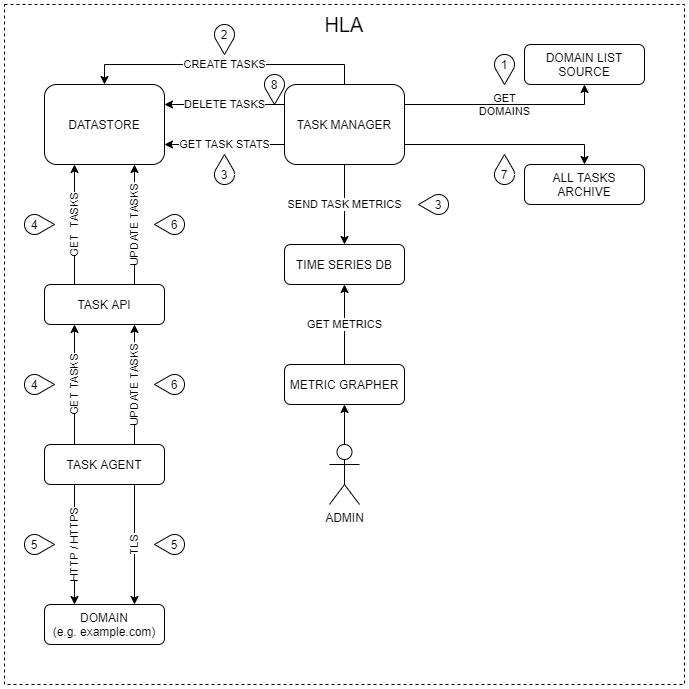
\includegraphics[scale=0.5]{../images/HLA_Pre_Implementation_v2.png} 
		\caption{High Level Design}
		\label{fig:hla_design}
	\end{center}
\end{figure}

\begin{table}[p]
  \begin{center}
    \begin{tabular}{|l|G|}  % <-- Alignments: 1st column left, 2nd middle and 3rd right, with vertical lines in between
      \hline
      \textbf{\#} & \textbf{Description}\\
      \hline
      1 & A list of domains will be acquired to scan against \\
      \hline
      2 & For each of the domains in the domain list, a task manager will create a ``task'', to be stored in a database, representing a domain to be scanned \\
      \hline
      3 & Metrics on the state of tasks will be sent to a time series database \\
      \hline
      4 & A task agent will poll an API for a new batch of tasks \\
      \hline
      5 & A task agent will scan a domain as stated in the task being processed \\
      \hline
      6 & A task agent will send the result of a domain scan to an API to be stored in a database \\
      \hline
      7 & A task manager, once all tasks are completed, will extract all tasks from the database to an archive file format \\
      \hline
      8 & A task manager, once all tasks are completed, will delete all the tasks from the database \\
      \hline
    \end{tabular}
%    \captionsetup{width=.75\textwidth}
    \caption{Descriptions for Figure \ref{fig:hla_design}}
    \label{table:hla_design} % label MUST be after caption https://stackoverflow.com/questions/1353120/referring-to-a-table-in-latex
  \end{center}
\end{table}

\clearpage
\newpage

\subsection{Implementation}
\label{section:Implementation}

This section describes the chosen technologies and resources for the implementation, shown in Figure \ref{fig:hla_design_implmementation}, of the design in section \ref{subsection:hld}.

\begin{figure}[h!]
	\begin{center}
		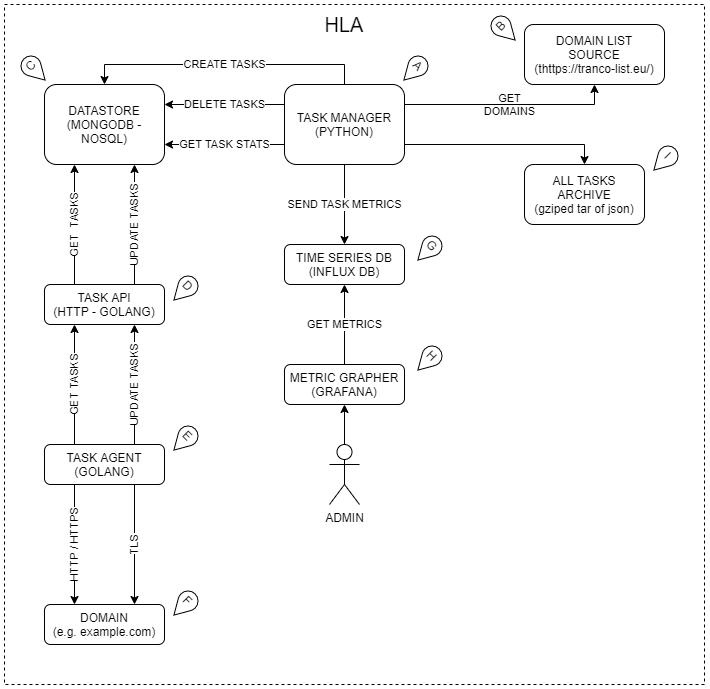
\includegraphics[scale=0.65]{../images/HLA_Implementation_v1_Entites.png} 
		\caption{High Level Design - Implementation}
		\label{fig:hla_design_implmementation}
	\end{center}
\end{figure}

\clearpage

\newpage

\subsubsection{[A] Task Manager}

The Task Manager performs the following tasks:

\begin{itemize}
	\setlength\itemsep{0.1em}
    \item Obtains the list of domains from the ``Tranco'' domain list source \newline (\texttt{https://tranco-list.eu/top-1m.csv.zip}).
    \item Create tasks directly in the Datastore (MongoDB).
    \item Create an archive of the tasks via the Task API.
    \item Delete tasks from the MongoDB database.
    \item Identify zombie tasks (tasks that have been marked as started but not complete after a certain amount of time).
    \item Generate task metrics and store them directly in the time series DB (Influx DB).
\end{itemize}

\noindent
The task manager was developed in python as it:

\begin{itemize}
	\setlength\itemsep{0.1em}
    \item Is a relatively high-level programming language which aids in being easier to learn than a more low-level language.
    \item Has many libraries and resources freely available online.
    \item There is a large global community generally willing to help each other.
    \item Being such a popular language, issues that one may come across may have already been encountered and solved already.
    \item Is cross platform, i.e. will run on any computer that has a python interpretor available to it.
\end{itemize}

\subsubsection{[B] Tranco Domains Source List}

As previously mentioned, similar research to this project have used pre-compiled lists, predominantly using the Alex Top Sites list \cite{Buchanan2018-xz,Chen2016-dl,Kumar2017-qw,Patil2017-bg,Ying2016-ag,Michael2015-hn,Van_Goethem2014-ao,Holz2020-ha,Poteat2021-zr}.

\vspace{0.3cm} \noindent
The research conducted by the Tranco team \cite{Le_Pochat2018-ql}, who provide the Tranco domain list \cite{noauthor_undated-mt}, compared several of the ``most popular domains'' lists and identified that domains present in the list can vary wildly on a day to day basis and are susceptible to influence by malicious actors.

\vspace{0.3cm} \noindent
As a result of this paper and that the Tranco list uses other top site lists to influence their list, the Tranco list \cite{noauthor_undated-mt} was chosen as the source for the domains to scan for this project.

\subsubsection{[C] Datastore}

The database is intended to only be an ephemeral store as it will only store the tasks until they have all been completed.

\vspace{0.3cm} \noindent
The data that will be returned by the task agent will be of arbitrary length and structure. A relational database is not the optimal choice as it is based on having one or more ``tables'' that relate to one another.

\vspace{0.3cm} \noindent
A NOSQL database is designed to store arbitrary length and a non pre-defined content structure.

\vspace{0.3cm} \noindent
The MongoDB database technology was chosen as it:

\begin{itemize}
	\setlength\itemsep{0.1em}
    \item A NOSQL database.
    \item Is relatively mature technology implementation.
    \item Has a community version (i.e. free).
    \item Many programming languages have pre-existing support (libraries).
    \item Has native support for unstructured data.
    \item Has detailed online documentation.
\end{itemize}

\subsubsection{[D] Task API}

The Task API is meant purely as a common interface for the task agent such that the task database can be changed without the need to modify the task agent.

\vspace{0.3cm} \noindent
The HTTP protocol was chosen as the interface to the API as it is a very well known and a standard protocol to use for an API.

\vspace{0.3cm} \noindent
The intended clients of the API is the Task Agent (for running and updating the tasks) and the Task Manager (for creating an offline archive once all tasks have completed for later analysis).

\vspace{0.3cm} \noindent
The Task API can perform the following functions:

\begin{itemize}
	\setlength\itemsep{0.1em}
    \item Allow a client to retrieve one or more tasks via a HTTP GET request.
    \item Allow the following task database filtering via url arguments when a HTTP GET request is made.
    \item Task Status (e.g completed).
    \item Task Unique ID.
    \item Sort by Unique ID.
    \item Allow a client to update one or more tasks via a HTTP POST request.
\end{itemize}

\vspace{0.6cm} \noindent
GO (also referred to as Golang) was chosen as the programming language to implement the API as it:
\begin{itemize}
	\setlength\itemsep{0.1em}
    \item Is a relatively low language which helps with improving performance.
    \item Is one of the easier lower-level languages to learn as it is one of the GO core principles to be able to pickup up the language quickly.
    \item Has the ability to run tasks concurrently (the more domains scanned concurrently the faster the scan of all domains can be completed).
    \item There are several community modules for GO to communicate with MongoDB (the chosen database for this project).
    \item Has numerous community modules for GO for the purpose of creating a HTTP API.
\end{itemize}

\subsubsection{[E] Task Agent}

The task agent obtains tasks from the Task API. A task contains the required information to allow the task agent to conduct scans against a domain.

\vspace{0.6cm} \noindent
Table \ref{table:task_agent_parameters} details the parameters of a Task Agent.
\newpage

\begin{table}[H]
  \begin{center}
  	\resizebox{\textwidth}{!}{
    \begin{tabular}{|c|c|D|E|}  % <-- Alignments: 1st column left, 2nd middle and 3rd right, with vertical lines in between
      \hline
      \textbf{Parameter} & \textbf{Data Type} & \textbf{Value(s)} & \textbf{Description} \\
      \hline
      max HTTP redirects & int & 10 (Golang default) & The number of HTTP redirects allowed \\
      \hline
      \UScore{max_concurrent_tasks} & int & 100 & The maximum number of tasks that can be running concurrently \\
      \hline
      \UScore{deny_domains} & array of strings & Domains not to be scanned & domains not to be scanned \\
      \hline
      \UScore{deny_ips} & array of strings & IPv4 addresses not to be scanned & IPv4 addresses not to be scanned \\
      \hline
      \UScore{dns_lookup_nameservers} & array of strings & ``open'' recursive DNS servers & A list of recursive DNS servers \\
      \hline
    \end{tabular}}
%    \captionsetup{width=.75\textwidth}
    \caption{Task Agent Parameters}
    \label{table:task_agent_parameters} % label MUST be after caption https://stackoverflow.com/questions/1353120/referring-to-a-table-in-latex
  \end{center}
\end{table}

\noindent
Section \ref{subsection:task_parameters} details the parameters of a task. \newline
Section \ref{section:task_flow} details the high level flow for the process of performing a domain scanning Task.

\vspace{0.3cm} \noindent
Appendix \ref{apdx:task_agent_tls_client} details TLS client capabilities of the Task Agent.

\vspace{0.3cm} \noindent
As with the Task API the Task Agent will use the programming language GO.

\subsubsection{[F] Domain}

This is the target domain of a task being performed by the Task Agent.

\subsubsection{[G] Time Series Database}

The Task Manager will create metrics about tasks and send them to the time series database. Time series databases are optimised for metrics that are time bound which is the type of metrics that is required to be stored. 

\vspace{0.3cm} \noindent
InfluxDB was the time series database technology implementation chosen as it is is relativity modern, quick to get up and running and has a community version available (free).

\subsubsection{[H] Metric Grapher}

A metric grapher allows the user to create charts from metrics. In the case of this project a metric grapher was used to generate basic graphs about the state of tasks for monitoring purposes from the metrics stored in the InfluxDB time series database.

\vspace{0.3cm} \noindent
Grafana was chosen as it is free, has built in support for communicating with InfluxDB, has an HTTP interface and offers the ability to create basic alerts.

\vspace{0.3cm} \noindent
Alerts were configured in Grafana to fire under the following conditions:

\begin{itemize}
	\setlength\itemsep{0.1em}
    \item If there were zombie tasks.
    \item If the number of tasks being processed dropped below a certain value over a specific amount of time for a task agent, if there were tasks waiting to be processed.
\end{itemize}

\subsubsection{[I] All Tasks Archive}

Once all tasks have been processed, the Task Manager will use the Task API to create a compressed archive file containing a JSON structured representation for each task.

\vspace{0.3cm} \noindent
This compressed archive is transferred to an archive file server for later analysis.

\subsection{Task Parameters}
\label{subsection:task_parameters}

A task has up to two parameters as shown in table \ref{task_paramters}.

\begin{table}[H]
  \begin{center}
    \begin{tabular}{|c|c|c|F|}  % <-- Alignments: 1st column left, 2nd middle and 3rd right, with vertical lines in between
      \hline
      \textbf{Name} & \textbf{Data Type} & \textbf{Mandatory} & \textbf{Description}\\
      \hline
      \textbf{fqdn} & string & Yes & A domain from the domain list provided by tranco-list.eu\\
      \hline
      \textbf{headers} & string & No & A JSON string of one or more HTTP client headers and values\\
      \hline
    \end{tabular}
%    \captionsetup{width=.75\textwidth}
    \caption{Task Parameters}
    \label{table:task_paramters} % label MUST be after caption https://stackoverflow.com/questions/1353120/referring-to-a-table-in-latex
  \end{center}
\end{table}

\noindent
All tasks will be using the same request headers as shown in table \ref{table:task_paramters_headers}. The header names and values were those present in the HTTP request from visiting the url \texttt{https://www.google.com} and were captured using chrome's browser developer tools.

\newpage

\noindent
This was done to best represent the standard request headers a browser would send to domain to thus have the best representation of response headers a user browsing the internet, would receive from a domain.

\begin{table}[t]
\footnotesize
  \begin{center}
    \begin{tabular}{|c|E|E|}  % <-- Alignments: 1st column left, 2nd middle and 3rd right, with vertical lines in between
      \hline
      \textbf{Name} & \textbf{Value} & \textbf{Description}\\
      \hline
      accept & text/html, application/xhtml+xml, application/xml; q=0.9,image/webp, image/apng, */*;q=0.8, application/signed-exchange; v=b3;q=0.9 & The accepted content types e.g html page.\\
      \hline
      accept-encoding & gzip, deflate, br & The accepted content encoding(s) e.g. gzip\\
      \hline
      accept-language & en-US,en;q=0.9 & The accepted languages e.g. en-US\\
      \hline
      sec-fetch-dest & document & Requested destination e.g. document\\
      \hline
      sec-fetch-mode & navigate & Differentiator for request type e.g. navigation or websocket\\
      \hline
      sec-fetch-site & none & If the request is coming from the same origin e.g. none (user-originated operation)\\
      \hline
      sec-fetch-user & ?1 & Sent for requests initiated by user activation\\
      \hline
      upgrade-insecure-requests & 1 & Signal to the server that an authenticated and encrypted response is preferred e.g. redirect to secure version of the site\\
      \hline
      user-agent & Mozilla/5.0 (Windows NT 10.0; Win64; x64) AppleWebKit/537.36 (KHTML, like Gecko) Chrome/91.0.4472.101 Safari/537.36 & Identification of requests application e.g. browser identification\\
      \hline
    \end{tabular}
%    \captionsetup{width=.75\textwidth}
    \caption{Task Parameters - Headers}
    \label{table:task_paramters_headers} % label MUST be after caption https://stackoverflow.com/questions/1353120/referring-to-a-table-in-latex
  \end{center}
\end{table}

\vspace{0.3cm} \noindent
All the headers in table \ref{table:task_paramters_headers} where carefully checked as to their purpose and if they were suitable to be included in order to obtain the best response from domains for the most relevant data to analyse from the perspective of a generic user browsing the internet.

\vspace{0.3cm} \noindent
The \texttt{user-agent} header is generally considered one of the most critical headers to use for HTTP requests to be associated with coming from a browser, rather than a backend service application, as almost all related research use this header \cite{Patil2017-bg,Buchanan2018-xz,Amann2017-co,Kotzias2018-wd,Poteat2021-zr,Van_Goethem2014-ao,Chen2016-dl,Kumar2017-qw,Michael2015-hn}.

\vspace{0.3cm} \noindent
The headers with the prefix \texttt{sec} are to enhance the premise that the request is coming from a user making the request manually in a browser. It could be argued that the \texttt{accept} headers are not needed however they should only give credit that the request is from a user rather than a service.

\subsection{Task Flow}
\label{section:task_flow}

This section describes the high level task flow once a task has been obtained from the Task API and is now to be processed.

\vspace{0.3cm} \noindent
The following describes the stages that task processing goes through if the task parameter \texttt{fqdn} had a value of \texttt{example.com}. This is shown graphically in figure \ref{fig:task_flow}.

\subsubsection{Stage 0 - Task Parameters}

The task parameters are checked for validity in the following way:
\begin{itemize}
	\setlength\itemsep{0.1em}
    \item If the parameter name is not valid for the task, abort the task
    \item If a mandatory parameter is not present, abort the task
\end{itemize}

\subsubsection{Stage 1 - Deny List}

The \texttt{fqdn} parameter value \texttt{example.com} is checked to see if it is on the task agents deny list, and if present the task is aborted and no further attempts will be made to process the task.

\subsubsection{Stage 2 - Resolve Domain}

DNS lookups for Stage 2 uses a round robin methodology with the DNS servers specified in the Task Agent parameter \texttt{\UScore{dns_lookup_nameservers}}, to reduce the load on any one DNS resolver.

\vspace{0.3cm} \noindent
A DNS request to lookup the \texttt{A records} (IPv4 addresses) of the fqdn parameter \texttt{example.com} is made.

\vspace{0.3cm} \noindent
If IPv4 addresses are returned, \texttt{example.com} is now referred to as the resolved domain resulting in Stage 2 being complete and processing moves to Stage 3.

\vspace{0.3cm} \noindent
If no IPv4 addresses are returned, a further DNS request to lookup the \texttt{A records} (IPv4 addresses) of the \texttt{www} subdomain of the fqdn parameter i.e. \texttt{www.example.com}.

\vspace{0.3cm} \noindent
If the DNS request made to \texttt{www.example.com} returns no IPv4 addresses, the task is aborted and no further attempts will be made to process the task.

\vspace{0.3cm} \noindent
If the DNS request made to \texttt{www.example.com} returns IPv4 addresses, \texttt{www.example.com} is now referred to as the resolved domain resulting in Stage 2 being complete and processing moves to Stage 3.

\vspace{0.3cm} \noindent
\textbf{NOTE:} For the purpose of describing the task flow, for the further stages, the resolved domain shall from here on out be assumed to have been determined to be \texttt{www.example.com} for the \texttt{fqdn} task parameter of \texttt{example.com}.

\subsubsection{Stage 3 - HTTP(S) Request}

A HTTP request is made to the resolved domain \texttt{http://www.example.com}.

\vspace{0.3cm} \noindent
Following redirects, if the last url in the redirect chain starts with \newline \texttt{https://} (e.g. \texttt{https://www.example.com/index.php}) Stage 3 is deemed complete and processing moves to Stage 4.

\vspace{0.3cm} \noindent
If the previous request did not result in a \texttt{https://} url a HTTPS request is made to the resolvable domain \texttt{https://www.example.com}.

\vspace{0.3cm} \noindent
Following redirects, if the last url in the redirect chain starts with \texttt{https://} (e.g. \newline \texttt{https://www.example.com/index.php}) Stage 3 is deemed complete and processing moves to Stage 4.

\vspace{0.3cm} \noindent
If the first request did result in a \texttt{http://} url (e.g. \texttt{http://www.example.com/index.php}), i.e. did not ultimately get redirected to a \texttt{https://} url, Stage 3 is deemed complete and processing moves to Stage 6 (skipping Stages 4 and 5 as they are only performed if a request ends in a HTTPS url).

\vspace{0.3cm} \noindent
If no \texttt{http://} or \texttt{https://} response is obtained from the resolved domain, Stage 3 is deemed to have failed and the task is aborted and no further attempts will be made to process the task.

\subsubsection{Stage 4 - TLS Versions}

TLS 1.0, 1.1, 1.2 and 1.3 connections are attempted against the domain of the last url in the redirect chain (e.g. domain \texttt{www.example.com} from last redirect url \newline \texttt{http://www.example.com/index.php}) from Stage 3.

\vspace{0.3cm} \noindent
The TLS version used for the HTTPS connection in Stage 3 is skipped as it has already been attempted and was successful.


\vspace{0.3cm} \noindent
Stage 4 is deemed complete and processing moves to Stage 5.

\subsubsection{Stage 5 - STS Preload}
\label{subsection:stage_5_STS}

This stage gathers the required data, such that a determination can be made at a later stage, if the domain of last url in the redirect chain (e.g. \texttt{http://www.example.com/index.php}) from Stage 3 meets the STS Preload requirements.

\vspace{0.3cm} \noindent
The STS Preload requirements are detailed in section \ref{section:STS_preload_bd}.

\vspace{0.3cm} \noindent
The following actions are performed on the base domain of the last url in the redirect chain from Step 3 and the results of which are recorded. The base domain of the url is determined by the use of the Golang library ``Golang.org/x/net/publicsuffix''. If any of the actions have already been performed in section 3, they are skipped as the results have already been captured:

\begin{itemize}
	\setlength\itemsep{0.1em}
    \item If the base domain (e.g. \texttt{example.com}) is running a HTTP server, on port 80, make a HTTP request to \texttt{example.com} i.e. \texttt{http://example.com}
    \item If the \texttt{www} subdomain has a DNS (A record) try and establish a TLS connection to the \texttt{www} subdomain \texttt{www.example.com}
    \item Make a HTTPS call to the base domain \texttt{https://example.com} and capture the HTTP headers
\end{itemize}


\subsubsection{Stage 6 - security.txt}

The path of the last url in the redirect chain (e.g. \texttt{http://www.example.com/index.php}) from Stage 3 is replaced with \texttt{.well-known/security.txt} i.e. \newline \texttt{http://www.example.com/.well-known/security.txt}.

\vspace{0.3cm} \noindent
A call is made to this url and if the \texttt{Content-Type} header is present with the value \texttt{text/plain} the body of the response is captured.

%\clearpage

%\newgeometry{top=7mm, bottom=0mm}
\begin{figure}[p]
	\begin{center}
%		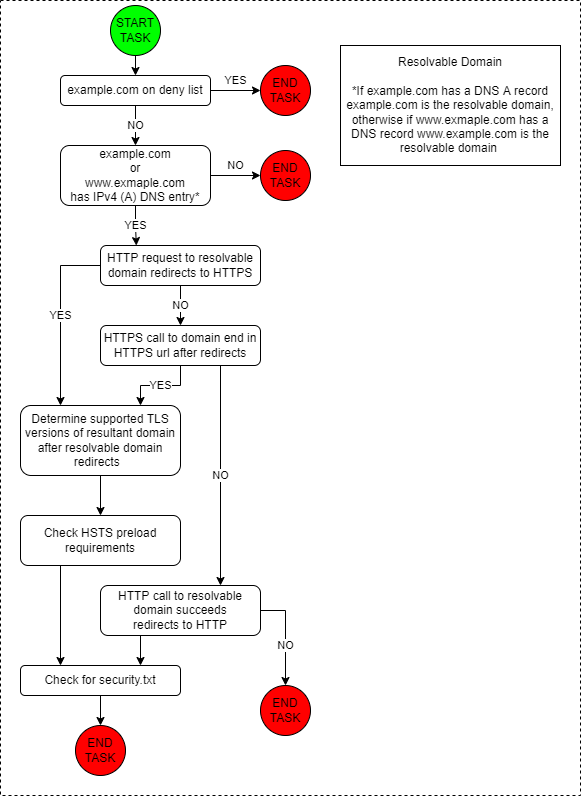
\includegraphics[scale=0.75]{../images/Task_Flowv2.png}
%		\includesvg[width=0.75](TaskFlow.svg)
%		\def\svgscale{0.4}
        \scalebox{0.47}{\subimport{../images}{TaskFlowv2fontv2.pdf_tex}}
		\caption{High Level Task Flow}
		\label{fig:task_flow}
	\end{center}
\end{figure}
%\restoregeometry

\clearpage
\newpage

\subsection{Deployment}

This section details how the implementation in section \ref{section:Implementation} was deployed.

\vspace{0.3cm} \noindent
The components as outlined in Section \ref{section:Implementation} were deployed using cloud infrastructure as detailed in Table \ref{table:implmentation_cloud}.

\begin{table}[H]
  \begin{center}
    \begin{tabular}{|c|c|c|c|c|c|}  % <-- Alignments: 1st column left, 2nd middle and 3rd right, with vertical lines in between
      \hline
      \textbf{Components} & \textbf{OS} & \textbf{\# vCPU} & \textbf{RAM} & \textbf{SSD} & \textbf{Qty}\\
      \hline
      MongoDB & FreeBSD 12.2 & 2 & 2GB & 25GB SSD & 1 \\
      \hline
      InfluxDB$+$Grafana & FreeBSD 12.2 & 1 & 1GB & 25GB SSD & 1 \\
      \hline
      Task API & FreeBSD 12.2 & 1 & 1GB & 25GB SSD & 1 \\
      \hline
      Task Agent & FreeBSD 13.0 & 1 & 512MB & 60GB SSD & 5 \\
      \hline
    \end{tabular}
%    \captionsetup{width=.75\textwidth}
    \caption{Cloud Infrastructure Deployment}
    \label{table:implmentation_cloud} % label MUST be after caption https://stackoverflow.com/questions/1353120/referring-to-a-table-in-latex
  \end{center}
\end{table}

\noindent
FreeBSD 13.0 was used for the task agents as it was the most recent version available at the time of deployment. There were no performance or security issues identified that required the effort to upgrade the components that remained on FreeBSD 12.2.

\vspace{0.3cm} \noindent
The number of Task Agents deployed was 5, such that the scanning could be conducted well within 24 hours to allow a reasonable amount of time to rectify issues should they occur. The average time for all 1 million domains to be scanned is approximately 11 hours.


\subsubsection{Monitoring}

A dashboard was created in Grafana to visualise the progress/status of scans. Over time several alerts were configured after issues were encountered. Figure \ref{fig:grafana_screenshot} shows a screen shot of the dashboard representing a time window of 7 days.

\newpage

\vspace{0.3cm} \noindent
There are several monitoring charts as detailed below:
\begin{itemize}
	\setlength\itemsep{0.1em}
    \item The Tasks Status By Agent chart displays the number of tasks of each task status' for a specific task agent. The "Agent" drop down box allows the user to select the task agent to be shown.
    \item The \textit{In Progress Tasks} / \textit{Completed Tasks} / \textit{Ready} / \textit{Error Cannot Retry} / \textit{Pending Ready} charts show the number of tasks, per task agent, of the charts title task status.
    \item Ready Delta - This is to monitor and alert for task agents that do not continually take new tasks if there are pending tasks.
    \item The Tasks in Zombie State is to monitor and alert for tasks that have started \textit{In Progress} but have not reached \textit{Completed} or \textit{Error Cannot Retry} status after a certain amount of time.
\end{itemize}



\begin{figure}[ht]
	\begin{center}
		\includegraphics[scale=0.48]{../images/Grafana.png} 
		\caption{Grafana Dashboard}
		\label{fig:grafana_screenshot}
	\end{center}
\end{figure}

\noindent
\clearpage

\subsubsection{Automation}

The Task Manager is scheduled to obtain the latest Tranco domain list and create tasks to scan each day at 0000 UTC. This will only occur if the previous day was completed successfully.

\vspace{0.3cm} \noindent
The Task Manager is scheduled to check if all the tasks have been completed between 1000 UTC to 2300 UTC. Once all tasks have been completed, they are collected to create the ``All Tasks Archive'' and then the tasks are deleted from the MonogDB datastore. Each ``All Tasks Archive'' is approximately 4GB in size.

\vspace{0.3cm} \noindent
A Task Agent continually look for new tasks to perform and run up to 100 concurrent tasks.

\subsubsection{Issues Encountered}
\label{subsection:issues_encountered}

\textbf{Zombie Tasks}

\vspace{0.2cm} \noindent
A zombie task is one where it is started but does not complete within a set amount of time. For this research the duration limit for a task deemed to be a zombie task is 120 minutes (2 hours). This occurred less than one task per 10 million tasks performed.

\vspace{0.2cm} \noindent
A scan outage for a duration of 27 days was caused by zombie tasks. A single task not completing will prevent the archive create process from starting. As a result changes were made such that when a low amount of zombie tasks were detected they were reset and re-attempted. All reset tasks completed successfully. If there were several zombie tasks detected this would raise alert and human intervention would be required to resolve the situation.

\vspace{0.2cm} \noindent
It was not looked into why zombie tasks occurred as the rate was so low it was not an efficient use of time and would not affect the research results as the tasks were successfully re-attempted.

\vspace{0.6cm} \noindent
\textbf{Data Loss}

\vspace{0.2cm} \noindent
An unexpected permanent loss of access to the storage location where the ``All Tasks Archives'' were stored, resulting in the permanent loss of 17 days worth of scan archives. Since this incident, scan archives are stored in more than one location within several hours of a scan archive being created.

\vspace{0.6cm} \noindent
\textbf{Programming}

\vspace{0.2cm} \noindent
Golang has, as of November 2021, a bug \cite{noauthor_undated-kp} where when a non standard HTTP code is received, it will cause Golang to panic and the program will terminate. There was a single domain that caused this issue and it was put in the deny list to overcome this issue.

\vspace{0.6cm} \noindent
\textbf{Development Work}

\vspace{0.2cm} \noindent
An 8 day scan outage was the result of development tasks being created in the same database as the production tasks. The archive creation process will not initiate unless there are the correct amount of tasks present. A procedure was put in place to remove development tasks after use.

\subsubsection{Missing Scans Overview}
\label{subsection:missing_scans_overview}

Table \ref{table:missing_scan_archives} summarises the extent of missing scan archives.

\begin{table}[H]
  \begin{center}
    \begin{tabular}{|D|D|I|I|}  % <-- Alignments: 1st column left, 2nd middle and 3rd right, with vertical lines in between
      \hline
      \textbf{Start Date} & \textbf{Duration} & \textbf{Cause} & \textbf{Action Taken}\\
      \hline
      24 Jan 2021 & 8 Days & Development tasks not removed after use which prevented scan archive creation & Added procedure to remove development tasks to mitigate further occurrences\\
      \hline
      16 March 2021 & 12 Days & Bug in archive creation process & Fixed bug and deployed updated scripts\\
      \hline
      31 July 2021 & 27 Days & One or more tasks did not complete preventing future scans to start & Enhanced alerting to detect long running tasks\\
      \hline
      17 September 2021 & 17 Days & Archive storage server permanently unavailable & Scan archives stored in multiple locations\\
      \hline
    \end{tabular}
%    \captionsetup{width=.75\textwidth}
    \caption{Missing Scan Archives}
    \label{table:missing_scan_archives} % label MUST be after caption https://stackoverflow.com/questions/1353120/referring-to-a-table-in-latex
  \end{center}
\end{table}

\newpage

%\vspace*{\fill}
%\begin{center}
%\begin{huge}
%Part IV - Security Mechanism Adoption Analysis
%\end{huge}
%\end{center}
%\vspace{\fill}
%
%\newpage


\chapter{Security Mechanism Overview}
\label{chap:sec_mech_overview}

\section{HTTPS}
\label{sec:https_bd}

This mechanism is analysed in section \ref{sec:ana_https_rdr}.

\vspace{0.3cm} \noindent
The S in HTTPS signifies that the HTTP protocol communication shall be over a secure channel, provided by the SSL/TLS protocols \cite{Rescorla2000-fs}. A URL starting with \texttt{https://} e.g. \texttt{https://example.com} signifies it will be using a SSL/TLS secure channel.

\vspace{0.3cm} \noindent
It has become quite common for websites to automatic redirect a user to a HTTPS url if the user enters or follows a HTTP url e.g. the URL \texttt{http://example.com} redirecting to \texttt{https://example.com}. This helps to enable the use of the HTTP protocol over a secure channel without the user having to actively seek out the HTTPS URL of a website (which most users are unlikely to do).

\section{TLS}
\label{sec:tls_bd}

This mechanism is analysed in section \ref{section:ana_ssl_tls}.

\vspace{0.3cm} \noindent
The SSL (Secure Socket Layer)/TLS (Transport Layer Security) protocols were designed to establish a secure communications channel between two entities e.g. a web browser and a website. Protocols such as HTTP can utilise SSL/TLS to secure its communication.

\vspace{0.3cm} \noindent
With each new version of SSL/TLS more security features were added in response to attacks against the protocols, weakness identified and the desire to make the protocols more secure.

\vspace{0.3cm} \noindent
The acronyms SSL and TLS are often used interchangeably to refer to the secure channel they provide, even though none of the SSL versions should be used any more due to the vulnerabilities and weaknesses of SSL 2.0 and SSL 3.0 \cite{Oppliger2016-ig}.

\subsection{Security Services}
\noindent The SSL/TLS mechanism provides several security services, as of the release of TLS 1.3 the main categories are: Confidentiality, Data Origin Authentication, Entity Authentication and Perfect Forward Secrecy.

\vspace{0.7cm} \noindent
\textbf{Confidentiality}

\noindent
Confidentiality is the protection of data such that only those who have been given authorisation can access the data.

\vspace{0.3cm} \noindent
Two entities should be able to establish a SSL/TLS connection between one another such that only these two entities can access the data data being sent over it. This should result in any third parties that are able capture the traffic from, not being able to recover the data being sent over the SSL/TLS channel \cite{Martin2017-sx}.

\vspace{0.7cm} \noindent
\textbf{Data origin authentication}

\noindent
The purpose of Data origin authentication is to establish the integrity of the SSL/TLS channel data. This is accomplished using message authentication codes (MAC)  or authenticated encryption with associated data (AEAD) algorithms \cite{Ristic2017-aj} which use keys derived from when the SSL/TLS connection was established.

\vspace{0.7cm} \noindent
\textbf{Entity Authentication}

\noindent
Entity Authentication provides the ability for an entity to prove their identity using mechanisms such as digital signatures.

\vspace{0.3cm} \noindent
In SSL/TLS entity authentication is mandatory and used to show that during the establishment of a SSL/TLS channel the client can verify that it really is communicating directly with the website/server they intended to. This is accomplished via the use of PKI (Public Key Infrastructure) with X.509 certificates and root stores. For further details on PKI please see \cite{Clark2013-sh,Holz2011-yv}.

\vspace{0.3cm} \noindent
It is optional for a client to prove its identity to the server using PKI during the establishment of the SSL/TLS channel.

\vspace{0.7cm} \noindent
\textbf{Perfect forward secrecy}

\noindent
Perfect forward secrecy ensures that if the private key that is paired with the certificate of a server/website that was compromised, any SSL/TLS traffic that was captured being sent to or from this server could not be decrypted with the private key being revealed. This is accomplished via the use of Ephemeral Diffie-Hellman key exchange \cite{Martin2017-sx}.

\vspace{0.3cm} \noindent
Perfect forward secrecy is mandatory as of TLS 1.3 and as such RSA key exchange was removed in TLS 1.3.

\subsubsection{SSL/TLS Versions}
\textbf{SSL 2.0 [1994]}

\noindent
Netscape Communications started developing a protocol, named Secure Socket Layer (SSL), for securing HTTP communications in 1993 \cite{Oppliger2016-ig}, due to the fact that when HTTP was first introduced it did not provide a means by which to secure its communications \cite{Oppliger2016-ig}.
Netscape Communications introduced SSL 2.0 in 1994 \cite{Oppliger2016-ig,Wu2016-nx}.

\vspace{0.7cm} \noindent
\textbf{SSL 3.0 [1995]}

\noindent
SSL 3.0 was introduced 1995 \cite{Ristic2017-aj,Oppliger2016-ig} and was a re-write of the SSL protocol, rather than additions/modifications, as many vulnerabilities and weaknesses had been identified in SSL 2.0 \cite{Ristic2017-aj,Wagner1996-fx}.

\vspace{0.3cm}\noindent
SSL 3.0 was eventually standardised as RFC6101 \cite{Freier2011-pt}.

\vspace{0.7cm} \noindent
\textbf{TLS 1.0 [1999]}

\noindent
In 1996 the IETF Transport Layer Security (TLS) Working Group was established \cite{Oppliger2016-ig,Farrell2010-kv} which produced TLS 1.0 as RFC4436 in 1999 \cite{Dierks1999-fn}.

\vspace{0.3cm} \noindent
TLS 1.0 was based on SSL 3.0 and introduced some enhancements and modifications \cite{Rescorla2001-gg}. Due to the changes made in TLS 1.0, it was allowed to be used by the US government as it gained FIPS approval \cite{Ristic2017-aj}.

\vspace{0.7cm} \noindent
\textbf{TLS 1.1 [2006]}

\noindent
TLS 1.1 was released as RFC4346 in 2006 \cite{Dierks2006-wu} which included a number of changes from TLS 1.0 some of which are:
\begin{itemize}
  \setlength\itemsep{0.1em}
  \item CBC (block mode) has to use explicit IVs which addressed the predictable IV weakness \cite{Ristic2017-aj}.
  \item \texttt{\UScore{bad_record_mac alert}} required to be used in the response when there are padding problems to protect against padding attacks \cite{Ristic2017-aj}.
  \item The addition of TLS extensions \cite{Ristic2017-aj} as described in RFC3546 \cite{Blake-Wilson2003-qv}
\end{itemize}

\vspace{0.7cm} \noindent
\textbf{TSL 1.2 [2008]}

\noindent
TLS 1.2 was released as RFC5246 in 2008 \cite{Dierks2008-uy} which included a number of changes from TLS 1.1 some of which are:
\begin{itemize}
  \setlength\itemsep{0.1em}
  \item IDEA and DES cipher suites were removed
  \item Authenticated encryption was added
  \item The extension \texttt{\UScore{signature_algorithms}} was added
\end{itemize}

\vspace{0.7cm} \noindent
\textbf{TLS 1.3 [2018]}

\noindent
TLS 1.3 was released as RFC8446 in 2018 \cite{Rescorla2018-wb} which is currently the latest published, as an RFC, TLS version as of 2022 which included a number of changes from TLS 1.2 some of which are:
\begin{itemize}
  \setlength\itemsep{0.1em}
  \item Removal of RSA for key exchange
  \item Removal of MD5, SHA-224 and DSA for Signature Algorithms
  \item Enforcement of Perfect Forward Secrecy
\end{itemize}


\section{Security.txt}
\label{sec:security_txt_bd}

This mechanism is analysed in section \ref{section:ana_security_txt}.

\vspace{0.3cm} \noindent
The security.txt is a text file placed at one of the following two locations hosted on a website:

\begin{itemize}
  \item Web-based services
  \item Filesystems
\end{itemize}

\vspace{0.3cm} \noindent
For websites, a file named ``security.txt'' \textbf{must} be placed in the path \texttt{/.well-known/security.txt} e.g. \texttt{https://example.com/.well-known/security.txt}.

\vspace{0.3cm} \noindent
It is also permitted to store a security.txt at the top level path e.g. \texttt{https://example.com/security.txt} or redirect to the \texttt{/.well-known/security.txt} path.

\vspace{0.3cm} \noindent
A response to a request of the security.txt file must respond with a \texttt{Content-Type} header with the value of \texttt{text/plain}, and served only over HTTPS.

\vspace{0.3cm} \noindent
The RFC is currently in the draft stage and seeing updates as recently as May 2021.

\vspace{0.3cm} \noindent
Example security.txt file:

\begin{lstlisting}
Contact: mailto:security@example.com
Expires: 2022-12-31T00:00:00.000Z
Encryption: https://example.com/pgp-key.txt
Acknowledgments: https://example.com/hall-of-fame.txt
Preferred-Languages: en, es, ru
\end{lstlisting}

\section{Content Security Policy}
\label{section:csp_bd}

This mechanism is analysed in section \ref{section:ana_csp}.

\vspace{0.3cm} \noindent
The Content-Security-Policy (CSP) is a mechanism of a web browser that allows the maintainer of a website to control, via the use of a policy, the resources that are allowed to be retrieved and or loaded by the browser. CSP is an evolution of the \textit{Same-Origin Policy (SOP)} browser mechanism.

\vspace{0.3cm} \noindent
The \texttt{Same Origin Policy} mechanism is rather restrictive and this is where Content Security Policy gives more control to website maintainers and developers.

\subsection{Development}

CSP is developed and maintained by The World Wide Web Consortium (W3C) \cite{Barth2012-ow}.
CSP Level 1 initial draft was published in 2012 \cite{Barth2012-ow} and finalised in 2015 \cite{Barth2015-ez}.
CSP Level 2 had its first draft in 2014 \cite{West2014-oe} and was finalised in 2016 \cite{West2016-ol} which included the following changes:
\begin{itemize}
  \setlength\itemsep{0.1em}
  \item base-uri, child-src, form-action, frame-ancestors, plugin-types directives added
  \item frame-src depreciated
  \item Inline scripts / stylesheets allowed via nonces
  \item New fields added to violation reports
\end{itemize}

\vspace{0.3cm} \noindent
CSP Level 3 first public draft introduced in 2016 \cite{West2016-xj} with the most recent draft in 2021 \cite{West2021-hi} and is currently in the working draft state which included the following changes:
\begin{itemize}
  \setlength\itemsep{0.1em}
  \item Spec re-written
  \item frame-src undepreciated (uses child-src if not present)
  \item manifest-src, worker-src directives added
  \item 'strict-dynamic' source expression added
  \item child-src substantially changed
  \item deprecation of the report-uri directive in favour of a more recent directive report-to
\end{itemize}


\subsection{Policy Delivery}
The CSP policy can be delivered either by the use of one of two HTTP headers (Content-Security-Policy and Content-Security-Policy-Report-Only) or in the \texttt{$<$meta$>$} element in the html body of a web page.

\subsubsection{CSP Directive}
A CSP Policy consists of one or more directives which are bound to a specific type of resource. For example, the script-src directive controls the restrictions, or lack thereof, for the location(s) scripts can be obtained, executed or loaded from. A CSP Directive can have of one or more values.

\vspace{0.3cm} \noindent
Should a directive be absent from a CSP Policy it is deemed to have no values i.e. ``open''. Configuring the default-src directive in a CSP policy cause most directives that are not present to inherit the values of the values of the default-src directive.

\vspace{0.3cm} \noindent
Table \ref{table:cpsdirectives1} details the directives from CSP Level 1 until CSP Level 3 29 June 2021. CSP Level 3 is still a working draft and as such until CSP Level 3 is finalised the data within table \ref{table:cpsdirectives1} may become inaccurate should there be any changes before CSP Level 3 is finalised.

\begin{table}[h!]
  \begin{center}
    \begin{tabular}{|l|J|c|}  % <-- Alignments: 1st column left, 2nd middle and 3rd right, with vertical lines in between
      \hline
      \textbf{Directive} & \textbf{Restrictive Context Sources} & \textbf{CSP Level}\\
      \hline
      default-src & Fall-back for interactions that are covered by CSP but not specified in other directives & 1\\
      \hline
      script-src & script sources: e.g. \texttt{$<$script$>$} elements, inline script blocks and XSLT stylesheets & 1 \\
      \hline
      object-src & Restricts the source of plugin requests/content & 1 \\
      \hline
      style-src & Style sources: e.g. \texttt{$<$style$>$} elements and \texttt{$<$link rel='stylesheet'$>$ elements} & 1\\
      \hline
      connect-src & The URLs being called from scripts e.g. XMLHttpRequest requests & 1 \\
      \hline
      img-src & Image sources: e.g. \texttt{$<$img$>$} elements & 1\\
      \hline
      media-src & Restricts the source of video/audio and related metadata & 1\\
      \hline
      frame-src & Restrict the source of loading resources into child browsing contexts (e.g. \texttt{$<$iframe$>$} elements) & 1\\
      \hline
      font-src & Restricts the source of font resources & 1\\
      \hline
      connect-src & Restricts source of script interface requests & 1\\
      \hline
      report-uri & Destination URI for sending CSP violates reports Deprecated as of CSP Level 3 in favour of \texttt{report-to} & 1\\
      \hline
      base-uri & Restrict URIs for a document's base element & 1.1\\
      \hline
      child-src & web worker sources and child browsing contexts (e.g. \texttt{$<$iframe$>$} elements) & 1.1\\
      \hline
      form-action & Restrict URIs for Form action target & 1.1\\
      \hline
      frame-ancestors & Restrict source of embedded child browsing contexts (e.g. \texttt{$<$iframe$>$} elements) & 1.1\\
      \hline
      plugin-types & Restricts the media type of plugins. No longer present as of \texttt{W3C Working Draft, 10 March 2021} \cite{noauthor_undated-xf} & 1.1\\
      \hline
      sandbox & Apply sandbox policy to a resource & 1.1\\
      \hline
      manifest & Restricts source of application manifests & 3 \\
      \hline
      prefetch-src & Restricts source of pre-fetched/pre-rendered resources & 3 \\
      \hline
      script-src-elem & Restricts source of $<$script$>$ elements only & 3 \\
      \hline
      script-src-attr & Restricts source of inline scripts (e.g. onclick) (not $<$script$>$ elements) & 3 \\
      \hline
      style-src-elem & Restricts source of $<$style$>$ and $<$link$>$ elements containing \texttt{rel="stylesheet"} only & 3 \\
      \hline
      style-src-attr & Restricts source of inline style & 3 \\
      \hline
      worker-src-attr & Restricts source of resources loaded as Worker, SharedWorker, or ServiceWorker & 3 \\
      \hline
      navigate-to & Restricts source of any navigations & 3 \\
      \hline
      report-to & Reporting group for sending CSP violates reports & 3 \\
      \hline
    \end{tabular}
%    \captionsetup{width=.75\textwidth}
    \caption{Summary of CSP directives}
    \label{table:cpsdirectives1} % label MUST be after caption https://stackoverflow.com/questions/1353120/referring-to-a-table-in-latex
  \end{center}
\end{table}

\subsection{Directives defined in other standards}

There are several CSP directives defined in other standards.

\vspace{0.7cm} \noindent
\textbf{upgrade-insecure-requests}

\vspace{0.3cm} \noindent
Converts any \texttt{http://} request made by the browser to use \texttt{https://} i.e. all \texttt{http://} requests will be forced to use \texttt{https://}.

\vspace{0.7cm} \noindent
\textbf{block-all-mixed-content}

\vspace{0.3cm} \noindent
Does not allow the browser to make any \texttt{http://} requests for assets if the page was loaded over \texttt{https://}. This directive is processed after the upgrade-insecure-requests is processed, should it be present.

\subsection{Source Lists}

Below are the types of sources for values of CSP directives.


\vspace{0.7cm} \noindent
\textbf{Keyword}

\vspace{0.3cm} \noindent
The values below are keywords that can be used as values for directives:
\begin{itemize}
  \setlength\itemsep{0.1em}
  \item \texttt{none} – does not allow the use of resources that apply to the directive in question.
  \item \texttt{self} – restricts the resources to the domain of the web page and does not include subdomains.
  \item \texttt{unsafe-inline} – Permits the resource to be inline, .e.g. a scripts code resides in a \texttt{$<$script$>$} element rather that in a separate file.
  \item \texttt{unsafe-eval} – Permits the use of mechanisms, such as \texttt{eval()}, which transform plain text into executable code.
  \item \texttt{unsafe-allow-redirects} – Used with the \texttt{navigate-to} directive. Not currently supported in browsers.
  \item \texttt{unsafe-hashes} – Allows the use of inline scripts if the script matches a hash in the \texttt{script-src} directive.
  
\end{itemize}

\noindent
Both \texttt{unsafe-inline} and \texttt{unsafe-eval} are deemed to be dangerous as inline resources and the use of mechanisms such as \texttt{eval()} are attack vectors for malicious actors, hence the use of the prefix \texttt{unsafe}.

\vspace{0.7cm} \noindent
\textbf{Host}

\vspace{0.3cm} \noindent
One or more ``hosts'' can be specified as values for a directive. The following are all valid examples of host values:
\begin{itemize}
  \setlength\itemsep{0.1em}
  \item domain.com
  \item *.domain.com
  \item https://*.domain.com:81
  \item domain.com/script.js
\end{itemize}

\vspace{0.5cm} \noindent
\textbf{Scheme}

\vspace{0.3cm} \noindent
Scheme values, referring the to protocol via which to access resources, may be used in directives. For example:

\begin{itemize}
  \setlength\itemsep{0.1em}
  \item http:
  \item https:
  \item data:
\end{itemize}

\vspace{0.5cm} \noindent
\textbf{Nonce}

\vspace{0.3cm} \noindent
A nonce can be used to allow inline resources to be allowed without the need to use the dangerous \texttt{unsafe-inline} keyword. The nonce would need to be included in both the CSP Policy directive and the inline resource.

\vspace{0.3cm} \noindent
For example if an in-line script was required, only scripts from the same origin are to be allowed, and the nonce was to be \texttt{MyRandomNonce}, then the CSP Policy would be:

\vspace{0.3cm} \noindent
\texttt{Content-Security-Policy: script-src 'self' 'nonce-MyRandomNonce'}

\vspace{0.3cm} \noindent
The inline script would also have the nonce:

\vspace{0.3cm} \noindent
\texttt{$<$script nonce="MyRandomNonce"$>$...$<$/script$>$}

\vspace{0.7cm} \noindent
\textbf{Digest}

\vspace{0.3cm} \noindent
A hash (digest) value can be used for scripts, the script-src directive, and non-script elements, such as the style-src directive. An example digest for the script-src directive:

\vspace{0.3cm} \noindent
\texttt{Content-Security-Policy: script-src 'sha256-MyHashDigest='}

\vspace{0.3cm} \noindent
If a digest value is present, each script element will be hashed and the resultant hash compared to the hash value in the directive and if a match occurs the script is deemed to be allowed.

\vspace{0.3cm} \noindent
The current hashing functions specified in CSP Level 3 are \texttt{sha256}, \texttt{sha368} and \texttt{sha512}.

\subsection{Reporting Directives}

\textbf{report-uri}

\vspace{0.3cm} \noindent
Upon a CSP Policy violation and a value is present for report-uri, the browser will send a report to the location specified for report-uri. The report is in the form of JSON document(s) and sent using the HTTP POST method.

\vspace{0.3cm} \noindent
As of the most recent CSP Level 3 working Draft (29 June 2021), report-uri is deprecated in favour of \texttt{report-to}.

\vspace{0.3cm} \noindent
An example report-uri configuration can be seen below:

\vspace{0.3cm} \noindent
\texttt{Content-Security-Policy: ...; report-uri https://report.example.com;}

\vspace{0.7cm} \noindent
\textbf{report-to}

\vspace{0.3cm} \noindent
Upon a CSP Policy violation and a value is present for report-to and the group is defined in the header \texttt{Report-To}, the browser will send a report to the location specified in the group configuration. The report is in the form of JSON document(s) and sent using the HTTP POST method.

\vspace{0.3cm} \noindent
An example report-to configuration can be seen below:

\vspace{0.3cm} \noindent
\texttt{Content-Security-Policy: ...; report-to <group name>}

\subsection{CSP Headers}

There are a number of CSP headers, shown below, that have been created leading up to the current \texttt{Content-Security-Policy} and \texttt{Content-Security-Policy-Report=Only} headers.

\begin{itemize}
  \setlength\itemsep{0.1em}
  \item Content-Security-Policy
  \item Content-Security-Policy-Report-Only
  \item X-Content-Security-Policy (Used by and now deprecated by Firefox browser)
  \item X-Webkit-CSP (Introduced and now deprecated by the chromium project since 2013 \cite{Google_undated-ct})
\end{itemize}


\subsection{Content-Security-Policy-Report-Only}

The header \texttt{Content-Security-Policy-Report-Only} behaves the same as \newline \texttt{Content-Security-Policy} with the exception that violations are only reported and not enforced. One of the main uses of this is when webmasters and developers are creating a CSP Policy and do not want to impact the end user experience until the policy is configured as desired.

\vspace{0.5cm} \noindent
Example basic CSP policy header: \texttt{Content-Security-Policy: default-src 'self'; script-src 'self' cdn.example.com; style-src 'self'}

\section{Strict Transport Security}
\label{section:STS_bd}

This mechanism is analysed in section \ref{section:ana_STS}.

\vspace{0.3cm} \noindent
The \texttt{Strict-Transport Security} response header (STS) is a mechanism that instructs the browser to load the website only over HTTPS and never HTTP \cite{Hodges2012-pe}.

\subsection{Directives}

\textbf{max-age}

\noindent
The duration, in seconds, the browser will honour the Strict-Transport Security request to only load the page over HTTPS.

\vspace{0.7cm} \noindent
\textbf{includeSubDomains}

\vspace{0.3cm} \noindent
Instructs the browser to also load any subdomains of the site only over HTTPS.

\vspace{0.7cm} \noindent
\textbf{preload}

\vspace{0.3cm} \noindent
Must be present if the site is to be preloaded via Google's STS preload service.

\vspace{0.3cm} \noindent
Example STS header configuration: \texttt{Strict-Transport-Security: max-age 31536000; includeSubDomains}.

\section{STS Preload}
\label{section:STS_preload_bd}

This mechanism is analysed in section \ref{section:ana_STS_preload}.

\vspace{0.3cm} \noindent
STS Preloading is a mechanism where a browser checks to see if the requested site is in a predefined list and if it is then the website must only be accessed over HTTPS.

\vspace{0.3cm} \noindent
Google maintains a predefined list, launched in 2010 \cite{Michael2015-hn}, of websites where the website owners/maintainers have requested to be added and required an email to be sent to a google  engineer to be included in the list \cite{Langley_undated-dm}. This service later gained a web portal in mid-2014 \cite{Michael2015-hn} for the request to be included in the preload list.

\vspace{0.3cm} \noindent
The Firefox browser generates its own preload list. Each domain from the preload lost maintained by Google is checked and if it meets all the preload requirements it is included in the Firefox preload list.

\vspace{0.3cm} \noindent
The following criteria must be met in order for a domain to qualify to be included in the preload list:

\begin{itemize}
  \setlength\itemsep{0.1em}
  \item The website has a valid certificate trusted by browsers.
  \item If the domain (e.g. \texttt{example.com}) is running a HTTP server, on port 80, it must redirect to the HTTPS on the same domain.
  \begin{description}
  \item[e.g.:] if \texttt{http://example.com} is accessible, it must redirect to \texttt{https://example.com}
  \end{description}
  \item All subdomains should be served over HTTPS, however only the \texttt{www} subdomain (e.g. \texttt{www.example.com}) is checked if present in DNS.
  \item A STS header (\texttt{Strict-Transport-Security}) is present on the base domain (e.g. \texttt{example.com}) for HTTPS requests with the following configuration:
  \begin{itemize}
    \item \texttt{max-age} directive must be no less than 31536000 seconds (i.e. 1 year).
    \item \texttt{includeSubDomains} directive must be present.
    \item \texttt{preload} directive must be present.
    \item Should the site redirect away when accessed over HTTPS, the site must have the STS header.
    \item Example STS header preload configuration: \texttt{Strict-Transport-Security: max-age 31536000; includeSubDomains; preload}.
  \end{itemize} 
\end{itemize}

\vspace{0.3cm} \noindent
If a domain in the preload list stops meeting the above criteria it runs the risk of being removed from the preload list.

\section{X Content Type Options}
\label{section:xcto_bd}

This mechanism is analysed in section \ref{section:ana_xcto}.

\vspace{0.3cm} \noindent
The \texttt{X-Content-Type-Options} header (XCTO) is used to enforce that the ``Multipurpose Internet Mail Extensions'' (MIME) specified in the \texttt{Content-Type} header (e.g. \newline 
\texttt{Content-Type: text/css}) match that of the requested resource \cite{Apple_undated-hz}.

\subsection{Directives}

\textbf{nosniff}

\vspace{0.3cm} \noindent
Denies requests under either of the two below conditions:

\begin{itemize}
  \setlength\itemsep{0.1em}
  \item A request has a destination of type script-like (one of \texttt{audioworklet}, \texttt{paintworklet}, \texttt{script}, \texttt{serviceworker}, \texttt{sharedworker}, or \texttt{worker}) and the \texttt{MIME} type (from the \texttt{Content-Type} header) is not a JavaScript \texttt{MIME} type.
  \item A request has a destination of type style and the MIME type (from the \texttt{Content-Type} header) is not \texttt{text/css}.
\end{itemize}

\vspace{0.3cm} \noindent
Example XCTO Header: \texttt{X-Content-Type-Options: nosniff}

\section{X Frame Options}
\label{section:xfo_bd}

This mechanism is analysed in section \ref{section:ana_xfo}.

\vspace{0.3cm} \noindent
The \texttt{X-Frame-Options} (XFO) response header is a mechanism that states whether or not a browser should load the url in question in any of the following html elements: \texttt{$<$frame$>$}, \texttt{$<$iframe$>$}, \texttt{$<$embed$>$}, or \texttt{$<$object$>$}.

\subsection{Directives}

\textbf{DENY}

\vspace{0.3cm} \noindent
The page must not be rendered in any of the following html elements: \texttt{$<$frame$>$}, \texttt{$<$iframe$>$}, \texttt{$<$embed$>$}, or \texttt{$<$object$>$}.

\vspace{0.7cm} \noindent
\textbf{SAMEORIGIN}

\vspace{0.3cm} \noindent
The page is allowed to be rendered in any of the following html elements: \texttt{$<$frame$>$}, \texttt{$<$iframe$>$}, \texttt{$<$embed$>$}, or \texttt{$<$object$>$}, if the origin of the page that contains the element is that of the page to be rendered in the element.

\vspace{0.7cm} \noindent
\textbf{ALLOW-FROM $<$uri$>$}

\vspace{0.3cm} \noindent
Behaves the same as the above SAMEORIGIN directive but only for \texttt{$<$frame$>$} elements. This directive is now deprecated and should not to be used.

\vspace{0.3cm} \noindent
Example XFO Header: \texttt{X-Frame-Options: DENY}

\section{Cross Origin Embedder Policy}
\label{section:coep_bd}

This mechanism is analysed in section \ref{section:ana_coep}.

\vspace{0.3cm} \noindent
The \texttt{Cross-Origin-Embedder-Policy} (COEP) header provides a mechanism that does not allow any cross-origin resources from being loaded unless explicitly allowed (via the use of Cross-Origin Resource Sharing or a Cross-Origin-Resource-Policy).

\subsection{Directives}
\textbf{unsafe-none}

\vspace{0.3cm} \noindent
Disables the mechanism allowing resources to be loaded without explicit permission being given. This is the default behaviour.

\vspace{0.7cm} \noindent
\textbf{require-corp}

\vspace{0.3cm} \noindent
Enables this mechanism only allowing resources being loaded from the same origin or from other origins that explicitly give permissions to do so (via the use of Cross-Origin Resource Sharing or a Cross-Origin-Resource-Policy).

\vspace{0.3cm} \noindent
Example COEP Header: \texttt{Cross-Origin-Embedder-Policy: require-corp}


\section{Cross Origin Resource Policy}
\label{section:corp_bd}

This mechanism is analysed in section \ref{section:ana_corp}.

\vspace{0.3cm} \noindent
The \texttt{Cross-Origin-Resource-Policy} (CORP) header provides a mechanism that restricts which origins are permitted to load a resource \cite{Apple_undated-au}.

\subsection{Directives}
\textbf{same-site}

\vspace{0.3cm} \noindent
If the request initiator's origin and the request destination's origins are of the same site then load the resource. For example, if the request initiator's origin is \newline \texttt{https://account.example.com/index.html} and the request destination is \newline \texttt{https://signin.example.com/script.js}, the resource can be loaded as both are of the same site \texttt{example.com}.

\vspace{0.7cm} \noindent
\textbf{same-origin}

\vspace{0.3cm} \noindent
If the request initiator’s origin and the request destination's origin are the same then load the resource. For example, if the request initiator’s origin is \texttt{https://blog.example.com} and the request destination is \texttt{https://blog.example.com}, the resource can be loaded as both are of the same origin \texttt{https://blog.example.com}.

\vspace{0.7cm} \noindent
\textbf{cross-origin}

\vspace{0.3cm} \noindent
The resource is allowed to be loaded regardless of the sites/origins involved.

\vspace{0.3cm} \noindent
Example COEP Header: \texttt{Cross-Origin-Resource-Policy: same-origin}

\vspace{0.3cm} \noindent
Example CORP Header: \texttt{Cross-Origin-Embedder-Policy: require-corp}

\section{Cross Origin Opener Policy}
\label{section:coop_bd}

This mechanism is analysed in section \ref{section:ana_coop}.

\vspace{0.3cm} \noindent
The \texttt{Cross-Origin-Opener-Policy} (COOP) header provides a mechanism that prevents the sharing of browsing contexts of a top-level document with cross-origin documents. For example, preventing a popup window from communicating to the web page (document) that opened the popup via the use of process isolation \cite{Apple_undated-gj}.

\subsubsection{Directives}
\textbf{unsafe-none}

\vspace{0.3cm} \noindent
Disables the mechanism unless the document (e.g. popup) uses this header with either of the two directives: \texttt{same-origin} and \texttt{same-origin-allow-popups}. This is the default behaviour.

\vspace{0.7cm} \noindent
\textbf{same-origin-allow-popups}

\vspace{0.3cm} \noindent
Allows the communication of a new window or tab (e.g. popup) to the originating page (document) if a COOP header is not present, or has the directive \texttt{unsafe-none}, on the new window or tab.

\vspace{0.7cm} \noindent
\textbf{same-origin}

\vspace{0.3cm} \noindent
Does not allow communication (isolates) from new windows or tab to the originating page (document) unless they are from the same origin. If not from the same origin they are placed in a separate browsing contexts.

\vspace{0.3cm} \noindent
Example COOP Header: \texttt{Cross-Origin-Opener-Policy: same-origin}

\section{Public Key Pins}
\label{section:hpkp_bd}

This mechanism is analysed in section \ref{section:ana_hpkp}.

\vspace{0.3cm} \noindent
This mechanism is analysed in section \ref{section:ana_hpkp}.
The \texttt{Public-Key-Pins} (HPKP) response header is a mechanism that permits a cryptographic public key to be advertised that must be matched to the website certificate presented during the SSL/TLS connection establishment otherwise the website will be prevented from loading/rendering.

\vspace{0.3cm} \noindent
There have been several issues with HPKP such as HPKP Suicide \cite{Chen2018-ft,Chuat2021-nf} or Ransom PKP \cite{Chuat2021-nf} which are forms of Hostile Pinning \cite{Evans2018-mi}

\vspace{0.3cm} \noindent
This header is now deprecated by most modern web browsers.

\subsection{Public-Key-Pins-Report-Only}
The \texttt{Public-Key-Pins-Report-Only} header does not enforce the pinning rather only sends violation reports.

\newpage

\chapter{Security Mechanism Adoption Analysis}
\label{chap:analysis}

\section{Scans Overview}
\label{section:scans_overview}

\subsection{Impact To Available Data For Analysis}

There are several gaps in the available scanning archives summarised in table \ref{table:missing_scan_archives}, detailed in section \ref{subsection:missing_scans_overview} and listed below:

\begin{itemize}
	\setlength\itemsep{0.1em}
    \item 24 Jan 2021 for 8 days
    \item 16 March 2021 for 12 days
    \item 31 July 2021 for 27 days
    \item 17 September 2021 for 17 days
\end{itemize}

\noindent
In the following sections these date ranges will be visible on certain charts. As the scanning has been for an extended period and any single time period is no longer than 27 days, it is believed it will not have a material impact on any trends identified.


\subsection{Analysis Methodology}

Each scan archive was processed, grouping related data together, such as all the security.txt files, to produce a JSON file to allow for easier analysis of the data.

\vspace{0.3cm} \noindent
A python application was created to parse these JSON files to produce further JSON files that were be used for creating charts.

\vspace{0.3cm} \noindent
A further python application was created to plot charts using the matplotlib charting library \cite{noauthor_undated-po}.

\vspace{0.3cm} \noindent
Each analysis section details how the data was processed.


\subsection{Domains Unable To Be Scanned}

As with other research, not all of the domains in the list of domains to be scanned were able to have a HTTP or HTTPS connection made to them.

\vspace{0.3cm} \noindent
On average the scanner was able to obtain a HTTP and or a HTTPS request 95\% of the time from the Tranco list of 1 million domains, shown in figure \ref{fig:failed_tasks}.

\begin{figure}[H]
	\begin{center}
        \subfloat[\centering Average percentage of domain scan final status]{\scalebox{0.80}{\subimport{../images}{domains_not_scanned-status_pie.pdf_tex}}}
        \subfloat[\centering Average percentage of domain scan failure cause]{\scalebox{0.80}{\subimport{../images}{domains_not_scanned-cannot_retry_pie.pdf_tex}}}
		\caption{Failed Tasks}
		\label{fig:failed_tasks}
	\end{center}
\end{figure}

\noindent
Of the 5\% of domains that the scanner was not able to obtain a HTTP or a HTTPS response, 51\% were due to differing errors, such as timeouts, in the establishment of a HTTP/HTTPS connection and the transmission of data across such a connection. The remaining 49\% was due to not receiving one or more IP addresses from the DNS lookup request.

%\restoregeometry

\clearpage 

\newpage

\section{HTTP(S) Redirection}
\label{sec:ana_https_rdr}

Background for this mechanism is detailed in section \ref{sec:https_bd}.

\subsection{Analysis}

\begin{figure}[H]
	\begin{center}
        \scalebox{0.90}{\subimport{../images}{http-https_redirects.pdf_tex}}
		\caption{HTTP(S) Redirections for Top 1 Million Domains}
		\label{fig:http_redirection}
	\end{center}
\end{figure}


\noindent
The research by \texttt{Buchanan et al} \cite{Buchanan2018-xz} found that in August 2015 only 6.7\% of sites when accessed over HTTP redirected to HTTPS and increased to 24.78\% in May 2017. The same research finds that in November 2020 the number of sites further increased to 56\% and continued this trend to reach 64.5\% in January 2022 as shown in table \ref{table:http_redirection} and figure \ref{fig:http_redirection}.

\newpage

\vspace{0.3cm} \noindent
This upward trend of HTTP to HTTPS redirection is slowing. However it is hoped that more sites continue to implement redirection such that future research does not show a plateau before nearly all sites in the top 1 Million redirect to HTTPS.

\vspace{0.3cm} \noindent
To some surprise there are a number of sites that redirect from HTTPS to HTTP, 3.5\% in November 2020 and  down to 1.7\% in January 2022. It is assumed that this is done on purpose, and that as the trend is on the decline that the reasons for implementing HTTPS to HTTP redirection are being overcome or not relevant any more.


\begin{table}[t]
\footnotesize
  \begin{center}
    \begin{tabular}{|l|D|D|c|c|}  % <-- Alignments: 1st column left, 2nd middle and 3rd right, with vertical lines in between
      \hline
      \textbf{Redirection} & \textbf{Buchanan et al} \cite{Buchanan2018-xz} August 2015 & \textbf{Buchanan et al} \cite{Buchanan2018-xz} May 2017 & November 2020 & January 2022 \\
      \hline
	  HTTP $>$ HTTP\textbf{S} & 6.7\% & 24.78\% & 56\% & 64.5\%\\
	  \hline
 	  HTTP\textbf{S} $>$ HTTP & NA & NA & 3.5\% & 1.7\%\\
      \hline
    \end{tabular}
    \caption{HTTP(S) Redirection}
    \label{table:http_redirection} % label MUST be after caption https://stackoverflow.com/questions/1353120/referring-to-a-table-in-latex
  \end{center}
\end{table}


\newpage

\section{TLS}
\label{section:ana_ssl_tls}

Background for this mechanism is detailed in section \ref{sec:tls_bd}.

\subsection{Purpose Overview}

\noindent
TLS is used to protect the data in transit between a users' browser and the website they are interacting with.

\vspace{0.3cm} \noindent
Changes to the data being sent across the TLS secure channel during its journey over the network (e.g the internet) are detected. The identity of the website is verified before the secure channel is established. The data being sent across the TLS secure channel is also encrypted. All of these properties of TLS are intnded to prevent entity in the middle attacks.

\vspace{0.3cm} \noindent There have been several vulnerabilities found in the SSL/TLS protocols, some of which are detailed earlier in section \ref{section:need_for_security_mechanisms}. 

\subsection{Analysis}

\subsubsection{Negotiated TLS Versions}

\begin{figure}[H]
	\begin{center}
        \scalebox{0.90}{\subimport{../images}{tls-tls_negotiated.pdf_tex}}
		\caption{TLS version negotiated for Top 1 Million Domains that support HTTPS}
		\label{fig:tls_negotiated}
	\end{center}
\end{figure}

\noindent
Figure \ref{fig:tls_negotiated} shows the negotiated TLS version of websites that ended with HTTPS URLs after HTTP redirection was completed. The scanner supported the following TLS versions when attempting to connect to a website with a HTTPS url:

\newpage
\clearpage

\begin{itemize}
  \setlength\itemsep{0.1em}
  \item TLS 1.0
  \item TLS 1.1
  \item TLS 1.2
  \item TLS 1.3
\end{itemize}

\noindent
No version of the legacy SSL technology is supported by the built in HTTP client in Go (the programming language used to create the scanner used to gather the data for analysis). The lack of support of SSL is not of concern as the use of SSLv3 (the last version of SSL that was widely used) currently is essentially 0\% as shown by the research by \textit{Kotzias et al} \cite{Kotzias2018-wd} which showed that analysing passively collected SSL/TLS usage, SSLv3 usage was 0.01\% of all TLS/SSL connections in February 2018.

\vspace{0.3cm} \noindent
As shown in figure \ref{fig:tls_negotiated}, November 2020 appears to show that it was just before this time that TLS 1.3 started to become the dominant TLS version negotiated, replacing TLS 1.2 as the dominant version. This assumption is enhanced by the research of \texttt{Holz et al} \cite{Holz2020-ha} which showed that in November 2019 from the analysis of passively collected TLS connection details, $\sim$79\% of connections were using TLS 1.2 with a downward trend and $\sim$19\% of connections using TLS 1.3 with an upward trend.

\begin{table}[H]
\footnotesize
  \begin{center}
    \begin{tabular}{|l|D|D|D|c|}  % <-- Alignments: 1st column left, 2nd middle and 3rd right, with vertical lines in between
      \hline
      \textbf{TLS Version} & \textbf{Kotzias et al} \cite{Kotzias2018-wd} July 2013 & \textbf{Kotzias et al} \cite{Kotzias2018-wd} August 2014 & \textbf{Holz et al} \cite{Holz2020-ha} November 2019 & January 2022 \\
      \hline
	  TLS 1.0 & $\sim$73\% & $\sim$48\% & $<$1\% & $<$1\%\\
	  \hline
	  TLS 1.1 & $\sim$17\% & $<$1\% & $<$1\% & $<$1\%\\
	  \hline
	  TLS 1.2 & $\sim$1\% & $\sim$48\% & $\sim$79\% & 35.2\%\\
	  \hline
	  TLS 1.3 & NA & NA & $\sim$19\% & 64.4\%\\
	  \hline
    \end{tabular}
    \caption{Negotiated TLS Versions}
    \label{table:tls_negotiated} % label MUST be after caption https://stackoverflow.com/questions/1353120/referring-to-a-table-in-latex
  \end{center}
\end{table}


\clearpage
\newpage


\subsubsection{Supported TLS Versions}

\begin{figure}[H]
	\begin{center}
        \scalebox{0.90}{\subimport{../images}{tls-tls_supported.pdf_tex}}
		\caption{TLS Versions Supported}
		\label{fig:tls_verions_supported}
	\end{center}
\end{figure}

\noindent
For each website that did support HTTPS, it was also checked to see which of the 4 TLS versions it supported. Figure \ref{fig:tls_verions_supported} shows how many domains supported the 4 TLS versions. The measurement of supported TLS versions was not observed in the research consulted for this project, indicating that it could be uncommon and as such this report may be one of only a handful that has conducted these measurements.

\vspace{0.3cm} \noindent
TLS 1.2 is in supported by over 99\% of domains. The reason for this is likely due to TLS 1.2 being the most recent TLS versions supported by some legacy devices and is likely to remain like this for many years to come. As one might expect, TLS 1.3 is on an upward trend going from 50\% in November 2020 and reaching 64\% in January 2022.

\vspace{0.3cm} \noindent
Both TLS 1.0 and TLS 1.1 look to follow the same downward trend with 44\% and 48\% in January 2022 respectively. As they follow the same trend it is likely due to when libraries and or applications are upgraded, rather than manual configuration changes to remove support for TLS 1.0 and TLS 1.1.

\vspace{0.3cm} \noindent
For the 0.2\% of websites that negotiate with TLS 1.0 or TLS 1.1 they did not support any version higher than that they negotiated with. There should not be a significant reason that TLS 1.2 and TLS 1.3 cannot be supported whilst also supporting TLS 1.0 and or TLS 1.1 for use by legacy devices. 

\vspace{0.3cm} \noindent
It is possible that websites are running old/outdated versions of applications, supporting only TLS 1.0 and or TLS 1.1, serving these websites and the maintainers are unaware or the updating of these older systems are of low priority. A reverse proxy would at least allow the public endpoint of such websites to use TLS 1.2 and TLS 1.3.

\vspace{0.3cm} \noindent
Table \ref{table:tls_supported_matrix} is a matrix for the different combinations of TLS versions supported by domains on 02 Jan 2022. The highest concentration of domains is for supporting both TLS 1.2 and TLS 1.3 which is quite encouraging. As stated previously, TLS 1.0 has a significant presence over TLS 1.1 shown as 2305 domains supporting TLS 1.0 alone.

\begin{table}[t]
%\small
  \begin{center}
    \begin{tabular}{|l|c|c|c|c|}  % <-- Alignments: 1st column left, 2nd middle and 3rd right, with vertical lines in between
      \hline
      \textbf{\# Domains} & \textbf{TLS 1.0} & \textbf{TLS 1.1} & \textbf{TLS 1.2} & \textbf{TLS 1.3} \\
      \hline
      9      & • & • &  & \\
	  \hline
      23     & • &  &  & •\\
	  \hline
      32     &   & • &   & •\\
	  \hline
      69     & • & • &   & •\\
	  \hline
      75     & • &   & • & •\\
	  \hline
      1579   & • &   &   & •\\
	  \hline
      2305   & • &   &   &  \\
	  \hline
      4888   &   &   &   & •\\
	  \hline
      12898  &   & • & • &  \\
	  \hline
      15954  &   & • & • & •\\
	  \hline
      137501 & • & • & • &  \\
	  \hline
      201151 & • & • & • & •\\
	  \hline
      261762 &   &   & • & •\\
	  \hline
    \end{tabular}
    \caption{Supported TLS Version matrix for 02 Jan 2022}
    \label{table:tls_supported_matrix} % label MUST be after caption https://stackoverflow.com/questions/1353120/referring-to-a-table-in-latex
  \end{center}
\end{table}


\subsection{Summary}

\noindent
The trend for negotiated TLS versions is going in the right direction, with TLS 1.3 being the dominant version, currently as this research began with an upward trend and as yet does not show sings of tapering off. TLS negotiations that result in either TLS 1.0 or TLS 1.1 is less than 1\% of all TLS negotiations.

\vspace{0.3cm} \noindent
The use of TLS 1.1 and TLS 1.0 were declining rapidly at the same rate at the end of 2020, however the trend is now starting to slow down which likely means TLS 1.1 and TLS 1.0 will still be in use s for some time.




\clearpage
\newpage

\section{Security.txt}
\label{section:ana_security_txt}

Background for this mechanism is detailed in section \ref{sec:security_txt_bd}.

\subsection{Purpose Overview}

\noindent
The ``security.txt'' mechanism is to aid in informing security researchers how to disclose security issues found on systems such as a domain hosting a HTTP(S) sever \cite{Foudil2021-vh}.

\vspace{0.3cm} \noindent
The primary emphasis of using a security.txt is that its location is known. Without knowing where to find the information required to report vulnerabilities, security researches may not be able to reach the right team in the organisation able to take action on the report for some time or even at all.

\vspace{0.3cm} \noindent
Security researches can spend quite a long time trying numerous channels such as Linkedin, contact pages on websites, guessing security email addresses. If private messaging attempts fail, some researchers resort to seeking assistance via twitter, however this also draws attention to there being a vulnerability on the organisation in the tweet which could allow malicious actors to discover and exploit the vulnerability before it is fixed.

\subsection{Scanning}

\vspace{0.3cm} \noindent
As the RFC Draft stated that ``\textit{For web-based services, organizations MUST place the "security.txt" file under the "/.well-known/" path}'' \cite{Foudil2021-vh} e.g. \newline \texttt{https://example.com/.well-known/security.txt} the scanner was initially configured to only try and obtain the security.txt from this location. The statement regarding an exception for legacy devices was missed when creating the scanner. The legacy exception was added in the 8th revision of the RFC dated November 19, 2019 \cite{Foudil2021-vh}.

\vspace{0.3cm} \noindent
At the end of November 2021 the research paper \textit{Who you gonna call? an empirical evaluation of website security.txt deployment} \cite{Poteat2021-zr} was discovered and found that 18\% of security.txt were found only at the top level path of the domain e.g. \newline \texttt{https://example.com/security.txt}.

\vspace{0.3cm} \noindent
As a result of this information, in December 2021 the scanner was reconfigured to attempt to capture at both paths. Even thought this would only allow a short time of data analysis it would allow, if only at least minimally, a comparison of results from this research to the research from \cite{Poteat2021-zr}.

\subsection{Parser}

A parser was created in python that processed security.txt request responses that had HTTP 2xx or 3xx status codes, split each security.txt on new line terminations and proceeded to process each line individually. Lines that started with a hash "\#" (\%x23) were skipped as these are comments as defined in the draft RFC.

\vspace{0.3cm} \noindent
If the first line was deemed to represent a non security.txt file, such as a html or php file, the entire security.txt file was skipped.

\vspace{0.3cm} \noindent
All non comment lines that were not able to have a field name determined were not processed any further and checked once all security.txt files had been processed. If any of the apparent non RFC format adhering lines were found to have been skipped, when they should not have been, the parser logic was analysed and corrected as needed until there we only non con-formant lines skipped.

\vspace{0.3cm} \noindent
As the scanner followed redirects, the parser kept track of the resultant domain of any such redirects and skipped processing a security.txt if the resultant domain had already had a security.txt processed.

\vspace{0.3cm} \noindent
If after processing a security.txt file no fields were detected, the security.txt was not deemed to be valid.

\vspace{0.3cm} \noindent
Contact values and expires date-times had multiple specially crafted regular expressions constructed in order to accurately categorise the field values, mainly due to many variants of the following:

\begin{itemize}
	\setlength\itemsep{0.01em}
    \item email obfuscation formats
    \item phone formats
    \item date-time formats
\end{itemize}

\vspace{0.3cm} \noindent
Even though \texttt{Acknowledgments} (American spelling) is the spelling used in the RFC \newline  \texttt{Acknowledg\textbf{e}ments} (British spelling - has an extra e), the parser considered it to be \newline \texttt{Acknowledgments} for the purposes of charting as the they are both valid spellings of the same word.

\vspace{0.3cm} \noindent
If a security.txt file was deemed to be con-formant it was hashed using the SHA256 hashing algorithm to determine how many unique security.txt files were present and how many domains shared the same security.txt file.

\vspace{0.3cm} \noindent
During the process of creating the parser it was noticed that some security.txt files had a dynamic value set for the Expires field (visiting the file manually on different occasions would show the expires time to be a constant time from the time of request). As this would affect the detection of unique security.txt, all Expires field lines were removed before hashing took place.

\newpage

\subsection{Analysis}

\begin{figure}[t]
	\begin{center}
        \scalebox{0.90}{\subimport{../images}{security.txt-by_rank.pdf_tex}}
		\caption{security.txt (only /.well-known path) by rank}
		\label{fig:security_txt_by_rank}
	\end{center}
\end{figure}

\subsubsection{Distribution by Rank}

\noindent
Figure \ref{fig:security_txt_by_rank} shows the percentage of domains that the scanner was able to identify having a valid security.txt at the path \texttt{/.well-known/security.txt} e.g. \newline \texttt{https://example.com/.well-known/security.txt}. The line chart is split by rank groups using the rank provided in the domains list file from tranco-list.eu for the day the scan was conducted.

\vspace{0.3cm} \noindent
Figure \ref{fig:security_txt_by_rank} closely matches, with a uniformly overall reduced percentage however, that of figure 1 in \cite{Poteat2021-zr}. It is not clear from \cite{Poteat2021-zr} whether the ranking always starts from 1 or from the previous smaller rank.

\vspace{0.3cm} \noindent
The ranks ranges in Figure \ref{fig:security_txt_by_rank} in this report are as stated in the legend domains from rank 1 to rank 100, rank 101 to 1000 and so on. The last rank is from 100001 to 1 million. Rank 1-100 from figure \ref{fig:security_txt_by_rank} should be comparative to that of the Top 100 of figure 1 in \cite{Poteat2021-zr} while taking into account the potential 18\% discrepancy.

\vspace{0.3cm} \noindent
The uniformly overall percentage difference is roughly the 18\% of security.txt files that are potentially missing from this reports figure \ref{fig:security_txt_by_rank} due to the finding in \cite{Poteat2021-zr} that 18\% of sites only serve a security.txt at their top level path.

\newpage

\begin{figure}[t]
	\begin{center}
        \scalebox{0.90}{\subimport{../images}{security.txt-by_root_vs_non_root.pdf_tex}}
		\caption{security.txt file locations}
		\label{fig:security_txt_by_root_vs_non_root}
	\end{center}
\end{figure}

\subsubsection{Distribution by Path}

\noindent
As noted in the scanning section above, the scanner was initially configured to only scan for security.txt at the \texttt{/.well-known} location. Figure \ref{fig:security_txt_by_root_vs_non_root} shows (from December 2021) onwards, that there are a significant about of security.txt only hosted at the top level path of the domain e.g. \newline \texttt{https://example.com/security.txt}. As of January 2022 46\% of security.txt are hosted at the top level path only.

\subsubsection{Unique Domains vs Unique Security.txt}

\noindent
Figure \ref{fig:security_txt_unique_vs_domains} shows the number of unique security.txt files and the number of all the security.txt files found on unique domains (separated by whether they are valid or not) that were found in the \texttt{/.well-known} location. The number of invalid security.txt files are a small percentage of all security.txt files and the majority of them are html documents unrelated to the security.txt mechanism.

\vspace{0.3cm} \noindent
The number of unique security.txt files is roughly half of all security.txt files found on unique domains. A reason for this could be that one organisation is responsible for multiple domains and uses a common security.txt for most and or all domains under their control.

\newpage

\begin{figure}[t]
	\begin{center}
        \scalebox{0.90}{\subimport{../images}{security.txt-unique_vs_non_unique.pdf_tex}}
		\caption{security.txt (only /.well-known path) Unique Domains vs Unique Files}
		\label{fig:security_txt_unique_vs_domains}
	\end{center}
\end{figure}


\begin{figure}[t]
	\begin{center}
        \scalebox{0.90}{\subimport{../images}{security.txt-fields_use_unique_files-root.pdf_tex}}
		\caption{unique security.txt (top level path) by field use}
		\label{fig:security_txt_by_fields_root_only}
	\end{center}
\end{figure}


\vspace{0.3cm} \noindent
Due to the large difference between the number of unique security.txt and number of unique domains further investigation was conducted to identify any large groupings of domains that used the same security.txt. From the 02 January 2022 scan, Google has the highest number of domains (198) with tumblr having (189) coming in a close second. The domains were grouped by the hash of the security.txt file. As one might expect the domains associated with Google predominantly started with \texttt{google.} e.g. \texttt{google.com}. The domains associated with tumblr had ``\textit{Please report abusive content (including spam, privacy violations, etc) at https://www.tumblr.com/abuse}'' in their security.txt file and did not appear to have a particular naming format, however the Hackerone link revealed that an organisation named ``Automatic'' manage the Hackerone representation.

\vspace{0.3cm} \noindent
Whilst this is nice to see that organisations look to be using unified configurations this does give another potential method by which to identify/fingerprint sites that are controlled by large organisations. This gives the opportunity to find sites with potentially weaker security (inherited from an acquisition for example) in order to laterally move to the parent organisations infrastructure.

\newpage

\subsubsection{Fields}

\noindent
A low amount of security.txt files (17\%) contained signatures which allow the security researcher to verify the legitimacy of the security.txt. It should be noted that the signature should be allowed to be verified using out of band methods (i.e. not a link in the security.txt itself) such as DNSSEC.

\begin{figure}[t]
	\begin{center}
        \scalebox{0.90}{\subimport{../images}{security.txt-fields_use_unique_files-well-known.pdf_tex}}
		\caption{unique security.txt (/.well-known path) by field use}
		\label{fig:security_txt_by_fields}
	\end{center}
\end{figure}

\vspace{0.3cm} \noindent
Figure \ref{fig:security_txt_by_fields} shows the field use of unique security.txt files. If a field is present more than once in a security.txt it is only counted once for the purposes of only showing if a field is present in a security.txt.

\vspace{0.3cm} \noindent
Figure \ref{fig:security_txt_by_fields_root_only} shows the field use distribution from December 2021 onwards for security.txt files found in the top level path location. Compared to the distributions in figure \ref{fig:security_txt_by_fields} they do not differ to such an extreme to discount the analysis from herein out which is only using the security.txt files found in the \texttt{/.well.known} location due to larger number of scans for analysis.

\vspace{0.3cm} \noindent
There are 8 defined fields in the RFC, 2 of which are mandatory (Contact and Expires shown in bold):

\begin{itemize}
	\setlength\itemsep{0.1em}
    \item Acknowledgments - links to acknowledge security researches for their efforts in reporting security vulnerabilities.
    \item Canonical - link to a canonical security.txt location.
    \item \textbf{Contact} - A method to use for reporting security vulnerabilities (e.g. email, phone and website URLs).
    \item Encryption - States or links on how to encrypt communication.
    \item \textbf{Expires} - The date-time after which that data present in the security.txt should not be used.
    \item Hiring - Link to a page detailing security related positions.
    \item Policy - Link to the vulnerability disclosure.
    \item Preferred-Languages - One or more languages, in order of preference, that the security report maybe be submitted in.
\end{itemize}

\vspace{0.7cm} \noindent
\textbf{Contact}

\noindent
Contact is a mandatory field and as such one would expect to see near 100\% usage and this is the case as can be seen in figure \ref{fig:security_txt_by_fields} which shows only that only 1.5-2\% of security.txt files do not have a \texttt{Contact} field present.

\begin{table}[H]
%\tiny
  \begin{center}
    \begin{tabular}{|c|c|}  % <-- Alignments: 1st column left, 2nd middle and 3rd right, with vertical lines in between
      \hline
      \textbf{Contact Type} & \textbf{Average Presence}\\
      \hline
      Email Address & 88\%\\
      \hline
      HTTP Link & 22\%\\
      \hline
      Phone Number & 1.6\%\\
      \hline
    \end{tabular}
    \caption{Presence of contact types from unique security.txts that contain a contact type}
    \label{table:security_txt_by_contact_type} % label MUST be after caption https://stackoverflow.com/questions/1353120/referring-to-a-table-in-latex
  \end{center}
\end{table}

\noindent
Table \ref{table:security_txt_by_contact_type} shows the average presence of the contact types detected in unique security.txt files. Even as the number of unique security.txt files increased over time as shown in figure \ref{fig:security_txt_unique_vs_domains}, the presence percentage deviation was less than 1\% for all contact types.

\begin{table}[H]
%\tiny
  \begin{center}
    \begin{tabular}{|c|c|}  % <-- Alignments: 1st column left, 2nd middle and 3rd right, with vertical lines in between
      \hline
      \textbf{Email Username} & \textbf{Average Usage}\\
      \hline
      security & 48\%\\
      \hline
      support & 2.2\%\\
      \hline
      info & 2.2\%\\
      \hline
      admin & 1.7\\
      \hline
      webmaster & 1.7\\
      \hline
    \end{tabular}
    \caption{Top 5 email usernames for security.txt email contacts}
    \label{table:security_txt_by_email_username} % label MUST be after caption https://stackoverflow.com/questions/1353120/referring-to-a-table-in-latex
  \end{center}
\end{table}

\noindent
The most prevalent email username used was \texttt{security}, as shown in table \ref{table:security_txt_by_email_username} which is of no real surprise due to the purpose of the security.txt.

\vspace{0.3cm} \noindent
There were several email addresses that were made obscure (obfuscated) which required multiple dedicated regular expressions to be created in order for the parser to detect them as email addresses. Some examples of email obfuscation observed are:

\begin{itemize}
	\setlength\itemsep{0.01em}
    \item security [at] example [dot] com
    \item security [@] example $<$do$t>$ com
    \item security [ a t ] example [ d o t ] com
    \item security[@]example.com
    \item security($<$remove me...$>$)at($<$remove me...$>$)\UScore{example_dot_com}
    \item the email address "security" on the domain "example.com"
\end{itemize}

\noindent
One reason why email addresses have been obfuscated is not wanting them to be identified on automated scraping/crawling. This could be a result of organisational policy or the person(s) responsible assumed that a person would be looking at the security.txt file and as such there was not much of a down side.

\begin{table}[H]
%\tiny
  \begin{center}
    \begin{tabular}{|c|c|}  % <-- Alignments: 1st column left, 2nd middle and 3rd right, with vertical lines in between
      \hline
      \textbf{Contact Count} & \textbf{Average Presence}\\
      \hline
      1 & 82.5\%\\
      \hline
      2 & 13.2\%\\
      \hline
      3 & 2.5\%\\
      \hline
      4 & 0.4\%\\
      \hline
      5 & 0.05\%\\
      \hline
      6 & 0.1\%\\
      \hline
    \end{tabular}
    \caption{Number of contacts present in a unique security.txt}
    \label{table:security_txt_by_contact_count} % label MUST be after caption https://stackoverflow.com/questions/1353120/referring-to-a-table-in-latex
  \end{center}
\end{table}

\noindent
Of the security.txt files that had one or more contacts, the majority contained only 1 contact as shown in table \ref{table:security_txt_by_contact_count}. Interestingly there were double the amount of security.txt files that contained 6 contacts than those that had 5 contacts.

\vspace{0.3cm} \noindent
Of the 1.5-2\% of security.txt files that did contain one or more fields but did not contain a \texttt{Contact} field, several did contain other non RFC contact fields including:

\begin{itemize}
	\setlength\itemsep{0.01em}
    \item openbugbounty field - openbugbounty is a not for profit organisation for the reporting of security vulnerabilities.
    \item email
    \item mailto
    \item contact us at
\end{itemize}

\vspace{0.7cm} \noindent
\textbf{Expires}

\noindent
\texttt{Expires} is a mandatory field and has a rather underwhelming presence starting in November 2021 of 0.7\% (the most least used field), going on to reach 4\% in mid March 2021. From March 2021 there is a marked increase in the rate at which \texttt{Expires} is included in security.txt files seen in figure \ref{fig:security_txt_by_fields} reaching 24\% presence at the end of December 2021 becoming the 3rd least used field.

\vspace{0.3cm} \noindent
If this trend continues, \texttt{Expires} will likely get close to 100\% use such as is with the \texttt{Contact} field.

\vspace{0.3cm} \noindent
There are several possible reasons that domains are not including the expires including:
\begin{itemize}
	\setlength\itemsep{0.01em}
    \item the administrative burden of regularly reviewing the security.txt.
    \item if a static date-time is used and it is left to expire, security researches may decide to seek conformation other than using the information in the contact field to verify the correct means of reporting a security vulnerability, thus delaying such reporting. If no expires is included then it cannot expire.
\end{itemize}


\noindent
Figure \ref{fig:security_txt_by_when_expires} shows that there are a minimal amount of security.txt files that have an expires value in the past (ranging from 0\% to $\sim$3\%). The number of security.txt files that expire in less than a year is trending down and those that are to expire greater than an year is increasing. This looks to indicate that expires values are being changed to last more than one year against the recommendation of the RFC, which is to have an expire value less than a year to avoid staleness.


\begin{figure}[t]
	\begin{center}
        \scalebox{0.90}{\subimport{../images}{security.txt-by_when_expires.pdf_tex}}
		\caption{Percentage of security.txt files (that use expires) by time until expires from scan date}
		\label{fig:security_txt_by_when_expires}
	\end{center}
\end{figure}

\vspace{0.7cm} \noindent
\textbf{Encryption}

\noindent
The RFC states that keys should not be included in security.txt files. Despite this, $\sim$0.7\% of unique files do include keys. This looks to indicate either that the majority are conforming to the RFC recommendation and or do not wish to include a key in the security.txt.

\begin{table}[H]
%\tiny
  \begin{center}
    \begin{tabular}{|c|c|}  % <-- Alignments: 1st column left, 2nd middle and 3rd right, with vertical lines in between
      \hline
      \textbf{Type} & \textbf{Presence}\\
      \hline
      HTTPS & $\sim$93.5\%\\
      \hline
      HTTP & $\sim$2\%\\
      \hline
      OpenPGP4 Fingerprint Reader & $\sim$3.0\%\\
      \hline
    \end{tabular}
    \caption{Percentage of encryption field value type of unique security.txt}
    \label{table:security_txt_encryption_type} % label MUST be after caption https://stackoverflow.com/questions/1353120/referring-to-a-table-in-latex
  \end{center}
\end{table}


\noindent
Table \ref{table:security_txt_encryption_type} shows three types of encryption reference: HTTPS, HTTP and OpenPGP4 Fingerprint Reader (openpgp4fpr). The RFC states that the \texttt{Encryption} field must begin with \texttt{https://}, however despite this OpenPGP4 Fingerprint Reader has a presence of $\sim$3.0\%. A reason for this could be that it was more convenient to use an OpenPGP4 Fingerprint Reader, however this might hinder the use of it if security researchers are not familiar with this scheme type. Should a website operator want to use OpenPGP4 Fingerprint Reader scheme, it is best placed in a separate web page such that instructions can be included on how to use such a scheme. 2\% of values use the scheme \texttt{http://} which is quite surprising given the purpose of a security.txt and being present in the \texttt{Encryption} field.

\vspace{0.7cm} \noindent
\textbf{Preferred-Languages}

\noindent
As one may expect there were many different languages (over 50) represented in the \texttt{Preferred-Languages} field. Table \ref{table:security_txt_preferred_languages} shows the presence of the top 5 languages for unique security.txt files.

\begin{table}[H]
%\tiny
  \begin{center}
    \begin{tabular}{|c|c|}  % <-- Alignments: 1st column left, 2nd middle and 3rd right, with vertical lines in between
      \hline
      \textbf{Language} & \textbf{Presence}\\
      \hline
      English & 99\%\\
      \hline
      German & 13\%\\
      \hline
      French & 11\%\\
      \hline
      Czech  & 13\%\\
      \hline
      Dutch & 4\%\\
      \hline
    \end{tabular}
    \caption{Percentage of encryption field value type of unique security.txt}
    \label{table:security_txt_preferred_languages} % label MUST be after caption https://stackoverflow.com/questions/1353120/referring-to-a-table-in-latex
  \end{center}
\end{table}

\noindent
English is the most prominent language which makes sense as that is also the most common language used for business. If a researcher did not speak English, or any of the other languages listed, they may be very well know someone who does in order to report an issue.

\vspace{0.7cm} \noindent
\textbf{Other RFC Fields}

\noindent
The remaining fields defined in the RFC that have not been analysed in this section are of less interest and as such only their relative presence in a security.txt was analysed and displayed in table \ref{table:security_txt_by_other_rfc_fields} and figure \ref{fig:security_txt_by_fields}.

\begin{table}[H]
%\tiny
  \begin{center}
    \begin{tabular}{|c|c|}  % <-- Alignments: 1st column left, 2nd middle and 3rd right, with vertical lines in between
      \hline
      \textbf{Field} & \textbf{Presence}\\
      \hline
      Acknowledgements & $\sim$7\%\\
      \hline
      Canonical & 30\%-33\%\\
      \hline
      Hiring & $\sim$21\%\\
      \hline
      Policy & 28\%-31\%\\
      \hline
    \end{tabular}
    \caption{Average field presence of remaining RFC fields in unique security.txt files}
    \label{table:security_txt_by_other_rfc_fields} % label MUST be after caption https://stackoverflow.com/questions/1353120/referring-to-a-table-in-latex
  \end{center}
\end{table}

\vspace{0.7cm} \noindent
\textbf{Non Standard Fields}

\noindent
There are a number of fields, many present in only a single security.txt, that appear in security.txt but are not defined in the RFC. Table \ref{table:security_txt_by_non_rfc_fields} details the top 5 most common of these non standard fields.

\begin{table}[H]
%\tiny
  \begin{center}
    \begin{tabular}{|c|c|c|}  % <-- Alignments: 1st column left, 2nd middle and 3rd right, with vertical lines in between
      \hline
      \textbf{Field} & \textbf{Presence} & \textbf{Inferred Use}\\
      \hline
      Signature & $\sim$4.5\% & Link to signature file\\
      \hline
      Openbugbounty & $\sim$3.5\% & Link to openbugbounty.org organisation page\\
      \hline
      Permission & $\sim$1.5\% & Permission to test vulnerabilities\\
      \hline
      Disclosure & $\sim$1\% & Type of public disclosure permitted\\
      \hline
      Sitemap & $\sim$1\% & HTTPS link to an XML file of the websites page structure\\
      \hline
    \end{tabular}
    \caption{Average field presence of remaining RFC fields in unique security.txt files}
    \label{table:security_txt_by_non_rfc_fields} % label MUST be after caption https://stackoverflow.com/questions/1353120/referring-to-a-table-in-latex
  \end{center}
\end{table}

\noindent
All of the \texttt{Permission} values appear to be set to \texttt{none} which would seem to indicate that permission is not given to perform testing for vulnerabilities against the site.

\vspace{0.3cm} \noindent
The \texttt{Disclosure} values were seen to be a HTTPS link, \texttt{Full}, \texttt{Partial} or \texttt{None} which would seem to indicate that if a security vulnerability were to be submitted the security researcher would act in good faith and adhere to this value in regards to the public disclosure of the security vulnerability found.

\subsection{Summary}

\noindent
The use of security.txt is quite minimal with 0.5\%, as of January 2022, of domains scanned having a valid security.txt file. This is not all to surprising as the RFC is still in the draft stage.

\vspace{0.3cm} \noindent
Approximately half  of all the valid security.txt files seen were unique, meaning that a large proportion of domains share the same security.txt file content.

\vspace{0.3cm} \noindent
Almost all security.txt files contained one or more contact which is the primary purpose of the security,txt mechanism to provide a contact point for security researchers to have an easy way to report  vulnerabilities.

\vspace{0.3cm} \noindent
As previously mentioned, one of the paths a securit y.txt file can be hosted at, as specified in the draft RFC, was not utilised by the scanner for the majority of the scans conducted. In any future studies, all paths specified in the latest version of the RFC should be utilised.

\newpage

\section{Content Security Policy}
\label{section:ana_csp}

Background for this mechanism is detailed in section \ref{section:csp_bd}.

\subsection{Purpose Overview}

CSP mainly provides mitigations for web applications against XSS Cross Site Scripting (XSS), data injection attacks and packet sniffing attacks. There are several basic policy settings that can be utilised for protection against such attacks.

\vspace{0.5cm} \noindent
\textbf{Restrict locations resources can be loaded from}

\vspace{0.3cm} \noindent
Using the script-src directive to only allow resources to be loaded from trusted sources is a great first step to prevent attackers from loading scripts. The additional use of sub resource integrity can be used to prevent supply chain attacks where the attacker takes control of a trusted source script.

\vspace{0.5cm} \noindent
\textbf{Remove the need to use unsafe directives}

\vspace{0.3cm} \noindent
Both \texttt{unsafe-inline} and \texttt{unsafe-eval} should be avoided especially with the  \texttt{script-src} and \texttt{style-src} directive to prevent attackers from injecting malicious script code into a website. Inline scripting is one of the biggest attack vectors for attackers trying to run scripts in the browser. An alternative to removing inline scripting is the use of the \texttt{Digest} keyword or the \texttt{Nonce} keyword to allow only specified inline scripts to run.

\vspace{0.5cm} \noindent
\textbf{Avoid using the data scheme}

\vspace{0.3cm} \noindent
Relatively tiny amounts of information can be used with the \texttt{data} schema and can be utilised for the purpose of triggering the download of malicious resources by attackers. A malicious script could be converted and placed into a \texttt{data} schema, injecting it into a page, leading to it being executed.

\vspace{0.5cm} \noindent
\textbf{Keep up to date with CSP Bypass Techniques}

\vspace{0.3cm} \noindent
CSP policy maintainers should keep up to date with CSP bypass techniques such as those described in  ``\textit{Complex Security Policy? A Longitudinal Analysis of Deployed Content Security Policies}'' \cite{Roth2020-hg}.

\subsection{Parser}

A parser was created in python which processed the value for a content security policy header. The parser checked all of the headers below of a scan result for the presence of a CSP header.

\begin{itemize}
	\setlength\itemsep{0.1em}
	\item Content-Security-Policy
	\item Content-Security-Policy-Report-Only
	\item X-Content-Security-Policy
	\item X-Webkit-CSP
\end{itemize}

\noindent
The CSP text was split on the \texttt{;} character which denotes that a directive configuration has ended. Each directive configuration was split on the space character which is the separator between directive configuration values.

\vspace{0.3cm} \noindent
A number of regular expressions were created to place each directive into one of the following categories as described in table \ref{table:directive_categories}.

\newpage

\begin{table}[t]
%\tiny
  \begin{center}
    \begin{tabular}{|c|c|c|}  % <-- Alignments: 1st column left, 2nd middle and 3rd right, with vertical lines in between
      \hline
      \textbf{Category} & \textbf{Description}\\
      \hline
      Allow All & The value \texttt{*}\\
      \hline
      Keyword & Any keyword value e.g. \texttt{self}\\
      \hline
      Scheme & Any scheme value e.g. \texttt{blob:}\\
      \hline
      Nonce & Any nonce value e.g. \texttt{nonce-MyRandomNonce}\\
      \hline
      Digest & Any digest value e.g. \texttt{sha256-MyHashDigest=}\\
      \hline
      Host & Any host value e.g. \texttt{*.example.com}\\
      \hline
    \end{tabular}
    \caption{CSP Directive Categories}
    \label{table:directive_categories} % label MUST be after caption https://stackoverflow.com/questions/1353120/referring-to-a-table-in-latex
  \end{center}
\end{table}

\vspace{0.3cm} \noindent
As the scanner followed redirects, the parser kept track of the resultant domain of any such redirects and skipped processing a CSP if the resultant domain had already had a CSP processed.


\subsection{Analysis}

\subsubsection{Distribution by Rank}

\noindent
Figure \ref{fig:csp_by_rank} shows the percentage of domains that the scanner was able to identify having a CSP header. The line chart is split by rank groups using the rank provided in the domains list file from tranco-list.eu for the day the scan was conducted.

\begin{figure}[H]
	\begin{center}
        \scalebox{0.90}{\subimport{../images}{csp-by_rank.pdf_tex}}
		\caption{CSP headers use by rank for unique domains}
		\label{fig:csp_by_rank}
	\end{center}
\end{figure}

\newpage

\vspace{0.3cm} \noindent
Each rank group shows a steady rise in the use of a CSP headers, with domain in the Rank of 1-100 group seeing the most use, which is an encouraging sign. There is a long way to go, however, to have the majority of sites using a CSP policy.

\vspace{0.3cm} \noindent
In the research by \texttt{Weissbacher et al} \cite{Weissbacher2014-vm} in March 2014 showed only 2\% of the sites ranked in the top 100 use CSP increasing to 7\% in the research by \texttt{Ying et al} \cite{Ying2016-ag} in June 2015 and as of January 2022 it is 36\% which is a marked increase.

\begin{table}[t]
\footnotesize
  \begin{center}
    \begin{tabular}{|l|I|D|c|}  % <-- Alignments: 1st column left, 2nd middle and 3rd right, with vertical lines in between
      \hline
      \textbf{HTTP Header} & \textbf{Weissbacher et al} \cite{Weissbacher2014-vm} March 2014 & \textbf{Ying et al} \cite{Ying2016-ag} June 2015 & Jan 2022 \\
      \hline
      Content-Security-Policy & 815 & 1241 & 83208\\
      \hline
      Content-Security-Policy-Report-Only & 35 & 180 & 15280\\
      \hline
      X-Content-Security-Policy & N/A & 111 & 1808\\
      \hline
      X-Webkit-CSP & N/A & 194 & 728\\
      \hline
    \end{tabular}
    \caption{Historical CSP Header Use}
    \label{table:csp_header_count} % label MUST be after caption https://stackoverflow.com/questions/1353120/referring-to-a-table-in-latex
  \end{center}
\end{table}

\begin{figure}[H]
	\begin{center}
        \scalebox{0.90}{\subimport{../images}{csp-header_use.pdf_tex}}
		\caption{CSP headers use by name}
		\label{fig:csp_by_rank}
	\end{center}
\end{figure}

\subsubsection{Distribution by Header}

\vspace{0.3cm} \noindent
Even though the \texttt{X-WebKit-CSP} and \texttt{X-Content-Security-Policy} CSP headers are now deprecated, there is still an increase in use from the \texttt{Ying et al} study \cite{Ying2016-ag} in June 2015 as shown in table \ref{table:csp_header_count}. The current (Jan 2022) overall percentage of use for these two headers, however, is less that 4\% of all the CSP headers combined.

\vspace{0.3cm} \noindent
Of the 4\% of domains that use the \texttt{X-WebKit-CSP} and \texttt{X-Content-Security-Policy} headers, only 13\% of these only use either of these two headers i.e. 87\% of domains that use \texttt{X-WebKit-CSP} and \texttt{X-Content-Security-Policy} also use the \texttt{Content-Security-Policy}.

\vspace{0.3cm} \noindent
The presumed reason that domains use both deprecated and current CSP headers is backwards comparability for older browsers. Other possible reasons could be that legacy configurations that have been added to rather than removing the deprecated headers, or tooling in use automatically configures the deprecated headers.

\vspace{0.3cm} \noindent
There is a spike in use from 20 December 2020 to 11 January 2021 for the \newline \texttt{Content-Security-Policy-Report-Only} header. The policy looks to be exclusively \newline \texttt{worker-src 'none'; report-uri /csp-report} and all the \texttt{server} header values were \textit{cloudflare}. Cloudflare provides many services for websites such as web increased performance via caching.

\vspace{0.3cm} \noindent
The CSP policy will send a report if a Worker, SharedWorker, or ServiceWorker script is attempted to be run. There does not seem to be any correlation between the websites other than using Cloudflare services. The short period the policy was deployed for, indicates that Cloudflare was doing some testing and or a beta program of some kind.

\vspace{0.3cm} \noindent
As of January 2022 33\% of domains that are using the \newline \texttt{Content-Security-Policy-Report-Only} header have not configured a \texttt{report-uri} or \texttt{report-to} directive, which results in reports not being sent upon policy violations. Developers might consider they do not as yet need to configure a reporting directive as they are still in the development phase and are using browser developer tools to identify policy violations.

\clearpage
\newpage

\subsubsection{Directives}

\begin{figure}[H]
	\begin{center}
        \scalebox{0.90}{\subimport{../images}{csp-content-security-policy-directive_use.pdf_tex}}
		\caption{Percentage of directives present in the \texttt{Content-Security-Policy}}
		\label{fig:csp_csp_by_directives}
	\end{center}
\end{figure}

Figure \ref{fig:csp_csp_by_directives} show the percentage of directives present in the \texttt{Content-Security-Policy}. The reason to single out \texttt{Content-Security-Policy} is that it is the only non deprecated header that is available for enforcing a CSP Policy as \texttt{Content-Security-Policy-Report-Only} merely reports on CSP violations.

\vspace{0.7cm} \noindent
\textbf{default-src}

\begin{table}[H]
%\footnotesize
  \begin{center}
    \begin{tabular}{|l|D|c|}  % <-- Alignments: 1st column left, 2nd middle and 3rd right, with vertical lines in between
      \hline
      \textbf{Keyword} & \textbf{Ying et al} \cite{Ying2016-ag} June 2015 & Jan 2022 \\
      \hline
      \texttt{*} & 14.10\% & 4.40\%\\
      \hline
      \texttt{none} & 2.74\% & 9.3\%\\
      \hline
      \texttt{self} & 42.55\% & 72.76\%\\
      \hline
      \texttt{unsafe-inline} & 5.80\% & 37.56\%\\
      \hline
      \texttt{unsafe-eval} & 6.69\% & 31.14\%\\
      \hline
      \texttt{unsafe-hashes} & N/A & 8.38\%\\
      \hline
    \end{tabular}
    \caption{Percentage of keyword use in default-src directive for unique CSP Policies}
    \label{table:csp_default-src-keyword} % label MUST be after caption https://stackoverflow.com/questions/1353120/referring-to-a-table-in-latex
  \end{center}
\end{table}

\clearpage
\newpage

\noindent
The distribution use of keywords has changed quite significantly since the study by \texttt{Ying et al} \cite{Ying2016-ag} in June 2015. It should be noted that there are also significantly more domains utilising CSP as well as the understanding of CSP will have increased which could very well have had an effect of keyword distribution change seen.

\vspace{0.3cm} \noindent
It is good to see that keyword \texttt{*} (essentially providing no protections) proportionally has reduced significantly from 14\% to 4\%. Unfortunately the proportional use of both \texttt{unsafe-inline} and \texttt{unsafe-eval} has over doubled.

\vspace{0.3cm} \noindent
The \texttt{self} keyword (restricting resources to the origin of the web page) sees a decent proportional increase from 43\% to 73\%. \texttt{unsafe-hashes} does not see that much use which is not surprising as it is a relatively new (introduced in 2018) keyword.

\vspace{0.7cm} \noindent
\textbf{script-src}

\begin{table}[H]
%\footnotesize
  \begin{center}
    \begin{tabular}{|l|D|c|}  % <-- Alignments: 1st column left, 2nd middle and 3rd right, with vertical lines in between
      \hline
      \textbf{Keyword} & \textbf{Ying et al} \cite{Ying2016-ag} June 2015 & Jan 2022 \\
      \hline
      \texttt{*} & 14.34\% & 6.99\%\\
      \hline
      \texttt{none} & 0.00\% & 0.12\%\\
      \hline
      \texttt{self} & 51.09\% & 83.70\%\\
      \hline
      \texttt{unsafe-inline} & 58.66\% & 86.83\%\\
      \hline
      \texttt{unsafe-eval} & 62.61\% & 79.17\%\\
      \hline
      \texttt{unsafe-hashes} & N/A & 1.41\%\\
      \hline
    \end{tabular}
    \caption{Percentage of keyword use in script-src directive for unique CSP Policies}
    \label{table:csp_script-src-keyword}  % label MUST be after caption https://stackoverflow.com/questions/1353120/referring-to-a-table-in-latex
  \end{center}
\end{table}

\noindent
It can be seen from table \ref{table:csp_default-src-keyword} that \texttt{self} has had a marked increase in proportional use from \texttt{Ying et al} \cite{Ying2016-ag} in June 2015. The use of keywords \texttt{unsafe-inline} and \texttt{unsafe-eval} have unfortunately significantly increased to over 87\% and 79\% respectively.

\vspace{0.3cm} \noindent
It is quite disappointing that the use of \texttt{unsafe-inline} and \texttt{unsafe-eval} is still so prevalent as setting these keywords allow a big attack vector for malicious actors. This indicates that website maintainers are struggling to be able to create CSP policies that are more restrictive but also do not impact the users experience, some may have even given up on the prospect.

\vspace{0.7cm} \noindent
\textbf{Reporting Directives}

\begin{figure}[t]
	\begin{center}
        \scalebox{0.90}{\subimport{../images}{csp-reporting_directives.pdf_tex}}
		\caption{Percentage of reporting directives present in the \texttt{Content-Security-Policy}}
		\label{fig:csp_by_reporting_directives}
	\end{center}
\end{figure}

\noindent
The reporting directives are a great way for policy developers to gain feedback on the polices, via the violation reports, being written and deployed for issues such as missing sources that need to be allowed, spelling mistakes in URLs and other flaws with a configuration to name a few.

\vspace{0.3cm} \noindent
There are online services dedicated to receiving and processing the csp violation reports which greatly aids in getting value from the reports and reduces the barrier to entry which can lead to more use of reporting directives.

\vspace{0.3cm} \noindent
The reports can also serve as a possible detection mechanism for malicious entities trying to or have already exploit a website.

\vspace{0.3cm} \noindent
The \texttt{report-uri} reporting directive, introduced with first publish CSP specification in 2012 and is in use by 15\% of domains using the \texttt{Content-Security-Policy} in January 2022 and the \texttt{report-to} directive is in use by 1.5\% of domains. The \texttt{report-uri} reporting directive is deprecated as of CSP3 which is yet to be published (it is still in a working draft stage) which would point as to the reason it is dominant over the \texttt{report-to} directive.

\vspace{0.3cm} \noindent
Figure \ref{fig:csp_by_reporting_directives} shows that the overall percentage use of the reporting directive is declining, however the number of domains using a CSP policy is increasing which indicates that figure \ref{fig:csp_by_reporting_directives} is showing as more domains start using a CSP policy they are not using a reporting directive or potentially domains are removing the reporting directives or even a combination of both.

\subsection{Summary}

\noindent
The ability to utilise a CSP policy has been available since 2015. We are now 7 years on and in January 2022 only 83 thousand domains (9\%) in the top 1 million ranked websites are using a CSP policy to protect their sites. This could indicate that website developers are finding it difficult to implement a CSP policy.

\vspace{0.3cm} \noindent
An alarming about of \texttt{script-src} directive configurations are still using the \texttt{unsafe} prefixed keywords (86\% that allow inline scripts) which allows one of the biggest attack vectors for websites that allow attacks such as cross site scripting attacks.

\vspace{0.3cm} \noindent
Websites are becoming more and more feature rich and being developed at an every increasing rate for many reasons such as staying competitive and demands from users. Libraries are often used along with numerous scripts created by the website developers which makes it very difficult or seemingly impossible to maintain a CSP policy that is both effective in protecting users as well as not impacting user experience (e.g. not blocking scripts that have changed and or added to add functionality to the website).

\vspace{0.3cm} \noindent
For a greater adoption of CSP, the frameworks and tooling used to create websites need to incorporate the facility to generate CSP polices as this would allow the "system" to know which scripts and external sources are needed thus already knowing the information required to create a policy.

\clearpage
\newpage

\section{Strict Transport Security}
\label{section:ana_STS}

Background for this mechanism was detailed in section \ref{section:STS_bd}.

\subsection{Purpose Overview}

\noindent
The STS header prevents an attacker trying to get the user to use HTTP to access the site so that the attacker could perform an entity in the middle attack, allowing the attacker to impersonate the user or just capture sensitive information to name only a few possibilities.

\vspace{0.3cm} \noindent
There is an issue however, in that a browser can only know to load over HTTPS when the header is received. On the first visit to a website an attacker could intercept a HTTP request to the website and keep the connection HTTP and thus the user would not get the STS header. To overcome this, preloading is required which was discussed in the previous section.

\clearpage
\newpage

\subsection{Analysis}

\begin{figure}[t]
	\begin{center}
        \scalebox{0.90}{\subimport{../images}{misc_headers-HSTS_overview.pdf_tex}}
		\caption{Number of Domains using the STS header and its directives}
		\label{fig:STS_overview}
	\end{center}
\end{figure}

\begin{table}[t]
\footnotesize
  \begin{center}
    \begin{tabular}{|I|D|H|c|}  % <-- Alignments: 1st column left, 2nd middle and 3rd right, with vertical lines in between
      \hline
      \textbf{Weissbacher et al} \cite{Weissbacher2014-vm} March 2014 & \textbf{Ying et al} \cite{Ying2016-ag} June 2015 & \textbf{Buchanan et al} \cite{Buchanan2018-xz} May 2017 & Jan 2022 \\
      \hline
      3,005 ($\sim$ 0.3\%) & 9,795 ($\sim$ 0.9\%) & 45,527 (5.4\%) & 200493 (21.1\%)\\
      \hline
    \end{tabular}
    \caption{Historical STS Header Use}
    \label{table:sts_header_count} % label MUST be after caption https://stackoverflow.com/questions/1353120/referring-to-a-table-in-latex
  \end{center}
\end{table}

\noindent
Figure \ref{fig:STS_overview} shows the usage of the STS header and its directives \texttt{max-age},  \texttt{includeSubDomains} and \texttt{preload}. It is difficult to see, however, the usage of the STS Header as directive \texttt{max-age} is present in almost every STS Header.

\vspace{0.3cm} \noindent
The usage of the directive \texttt{includeSubDomains} is consistently 40\% of all directives used. Modern websites and applications can have a vast amount of sub-domains and as such will take time to make them all HTTPS if not already. This can be a major factor in the relatively low use of this directive.

\vspace{0.3cm} \noindent
There are many more sites that have the \texttt{preload} directive set (21.5\%) than are in Google's preload list (3.5\% - shown in figure \ref{fig:STS_overview} as ``Preloaded Domains''). This could be websites preparing to be added to the preload list but as yet are not ready to meet the preload requirements. Currently there is no known use for using the \texttt{preload} directive other than being included in Google's preload list.

\clearpage
\newpage

\begin{figure}[t]
	\begin{center}
        \scalebox{0.90}{\subimport{../images}{misc_headers-HSTS_max_age.pdf_tex}}
		\caption{Duration groupings of the \texttt{max-age} directive}
		\label{fig:STS_max-age}
	\end{center}
\end{figure}

\noindent
Figure \ref{fig:STS_max-age} shows groups of the duration of the \texttt{max-age} directive. The most common duration is 1-3 years which is not unsurprising as the RFC states a value of 1 year. The upward trend is in the 1-3 years bracket which indicates that as sites add a STS header they are doing so with at least a year for the \texttt{max-age} directive.

\vspace{0.3cm} \noindent
This shows confidence that website maintainers are intending to keep their websites HTTPS for the foreseeable future.

\vspace{0.3cm} \noindent
As of January 2022 5\% of the \texttt{max-age} directive values are set to a value of 0, down from 6\% in November 2020. This essentially is ``opting out'' of the STS mechanism itself.

\vspace{0.3cm} \noindent
In table \ref{table:sts_header_count} it can be seen that there has been a near 5 fold increase in the use of the STS header from May 2017.

\subsection{Summary}

\noindent
As of January 2022 21.1\% of the top 1 million domains are using the STS header with an upward trend. This is quite promising to see and it is hoped the trend continues.


\vspace{0.3cm} \noindent
The most common value for the \texttt{max-age} directive is 1-3 years and a number of domains are using a value of 0 which means they are now actively opting out of the STS mechanism perhaps due to some endpoints not available over https as yet.


\clearpage
\newpage

\section{STS Preload}
\label{section:ana_STS_preload}

Background for this mechanism was detailed in section \ref{section:STS_preload_bd}.

\subsection{Purpose Overview}

\noindent
The main reason for STS Preloading is to ensure the first time a user visits a website it is over HTTPS. Without preloading, should a user visit the site the first time over HTTP, an attacker could intercept the traffic and perform malicious actions such as the entity in the middle attack as described in section \ref{subsection:entity_in_the_middle}.

\subsection{Parser}

\noindent
The scanner was not initially configured to capture all the required information to be able to evaluate the conformance to the preload requirements. In March 2021 the base redirect and www subdomain check were added to the scanner.

\vspace{0.3cm} \noindent
The parser was configured to only analyse domains that were specifically added to the preload list. This is due to entire TLDs (e.g. .app, bank and .dev) being configured in the STS preload list and thus domains of these TLDs were not necessarily set up to meet the preload list criteria.

\vspace{0.3cm} \noindent
In the preload commit (Tue Nov 09 22:54:06 2021) there are 34 TLDs configured. This means that any site that is of one of these preload lists is preloaded (i.e. the domain itself is not in the preload list only the TLD)

\vspace{0.3cm} \noindent
All of the STS preload lists were obtained from chromium.googlesource.com and the most recent list preceding the time of a scan was used to identify if a domain was preloaded or not.

\vspace{0.3cm} \noindent
A random selection of domains that the parser identified as both meeting the preload criteria and not meeting the preload criteria were checked on the https://STSpreload.org/ website for verification that the parser was working as intended.


\clearpage
\newpage


\subsection{Analysis}

\begin{figure}[t]
	\begin{center}
        \scalebox{0.90}{\subimport{../images}{HSTS_preload-overview.pdf_tex}}
		\caption{STS Preload Overview}
		\label{fig:STS_preloaded_overview}
	\end{center}
\end{figure}

\subsubsection{Preload Criteria Conformity}

\noindent
Figure \ref{fig:STS_preloaded_overview} shows an overall summary of the current state of top 1 million domains that are in the preload list managed by Google. The number of preloaded domains is quite a low percentage. As of January 2022 only 0.72\% of the top 1 million domains were preloaded.

\vspace{0.3cm} \noindent
The most recent STS preload list is from February 2022, as of January 2022, which contains 157192 (up from 1258 in 2010 \cite{Michael2015-hn}) entries which would seem to indicate that most of the preloaded domains are not in the top 1 million most popular domains.

\vspace{0.3cm} \noindent
The low amount of sites that are preloaded in the top 1 million most popular domains could be due to that the majority of sites being maintained by individuals with an interest in security and thus not likely to be a very popular domains compared to all the site on the internet.

\vspace{0.3cm} \noindent
As of January 2022 38\% of domains preloaded do not meet the preload requirements anymore. This is rather a high percentage and these domains are at risk of being removed as per the message displayed on STSpreload.org when checking a domain that no longer meets the preload requirements: \textit{``Status: $<$domain$>$ is currently preloaded, but no longer meets the requirements. It may be at risk of removal.''}.

\vspace{0.3cm} \noindent
Domains in the preload list that no longer meet the criteria and were in the preload list before the requirements were formally documented and the web portal rolled out in 2014, are not subject for removal from the preload list however.

\vspace{0.3cm} \noindent
Any data/publications detailing actual removal of domains due to them no longer meeting the requirements was unable to be identified.

\subsubsection{Criteria Not Met}

\begin{figure}[t]
	\begin{center}
        \scalebox{0.90}{\subimport{../images}{HSTS_preload-preloaded-not_all_criteria_met.pdf_tex}}
		\caption{Criteria not met for preloaded domains}
		\label{fig:STS_preloaded_criteria_not_met}
	\end{center}
\end{figure}

%\vspace{0.3cm} \noindent
%\cite{Michael2015-hn} Upgrading HTTPS in Mid-Air

\vspace{0.3cm} \noindent
Figure \ref{fig:STS_preloaded_criteria_not_met} shows the percentage of each criteria not met for domains that are preloaded from those that were scanned. The most prevalent criteria not met  was the lack of presence of the STS header followed by not redirecting from HTTP to HTTPS on the base domain.

\vspace{0.5cm} \noindent
\textbf{No Base Redirect}

\vspace{0.3cm} \noindent
If a website is running a HTTP server on its base domain on port 80 it must redirect to HTTPS on the same domain. For example of the base domain of \texttt{https://blog.example.com} is \texttt{example.com}. If a HTTP connection was able to be made to \texttt{http://example.com} it must then redirect to \texttt{https://example.com}.

\vspace{0.3cm} \noindent
As of January 2022 12.6\% of preloaded domains not longer redirect correctly from the base domain. A reason for this could be that the redirect was changed from redirecting to the base domain over HTTPS e.g. \texttt{https://example.com} but to the main url of the website such as \texttt{https://wwww.example.com} to save a redirect to the desired main website url for the end user.

\vspace{0.5cm} \noindent
\textbf{Subdomain not HTTPS}

\vspace{0.3cm} \noindent
The \texttt{includeSubdomains} parameter must be included on the STS header, meaning that all subdomains of the base domain will be forced to load over HTTPS. Only the www subdomain is checked to see if it has a DNS entry and subsequently checked if the domain supports HTTPS on the www subdomain e.g. \texttt{https://www.example.com}.

\vspace{0.3cm} \noindent
As of January 2022 less than 0.1\% of preloaded domains no longer use HTTPS on the www subdomain. This is not at all unsurprising, as it is unlikely that the www subdomain would have HTTPS support removed after it has been preloaded since it would be a primary subdomain to check for issues with HTTPS during the stage of making a domain preload compliant.

\vspace{0.5cm} \noindent
\textbf{STS Header}

\vspace{0.3cm} \noindent
\textit{- No STS Header}

\vspace{0.3cm} \noindent
By far the most prevalent reason that a domain no longer met the preload criteria was a missing STS header. Many websites have numerous subdomains and it can be hard to keep track of all that are in use. Those managing the security aspect may not be aware of all the subdomains and by preloading the base domain could have caused issues if one or more subdomains were configured with only HTTP or invalid HTTPS configurations. This would lead to the request to have the base domain removed from the preload list.

\vspace{0.3cm} \noindent
\textit{- Max Age too short}

\vspace{0.3cm} \noindent
4.2\% of preloaded domains that presented a STS header, have a \texttt{max-age} directive value of less than one year (31,536,000 seconds). This also happens to be the value given in the STS RFC \cite{Hodges2012-pe}.

\vspace{0.3cm} \noindent
For 02 January 2022 the most common duration under a year was 180 days (6 months). There were also 3 domains that presented a max-age of 31104000 which is only 5 days below the required 365 days. 20 domains used a value of 0, essentially ``opting out'' of both the preloading and STS mechanism itself.

\vspace{0.3cm} \noindent
\textit{- Missing preload}

\vspace{0.3cm} \noindent
1.6\% of preloaded domains did not provide the directive \texttt{preload} in the STS header. As this directive is only used for the purpose of preloading, one might assume that this was done on purpose indicating that preloading was not longer desired.

\vspace{0.3cm} \noindent
\textit{- Missing includeSubdomains}

\vspace{0.3cm} \noindent
1.8\% of preloaded domains do not include the \texttt{includeSubdomains} directive and 0.8\% are missing both the \texttt{includeSubdomains} directive and the \texttt{preload} directive.

\subsection{Summary}

\noindent
The usage of STS Preloading is as yet not all that common with 0.72\% of the top 1 million domains currently utilising it.

\vspace{0.3cm} \noindent
Of the domains that do use STS Preloading, 38\% no longer meet the requirements which could result in their removal from the list thus removing the extra security layer the STS Preloading mechanism provides. As of January 2022, not having a STS header was 30\% of all reasons that a domain no longer met the preload requirement meaning they have opted out of both the STS header protection and STS Preloading.

\newpage

\section{X Content Type Options}
\label{section:ana_xcto}

Background for this mechanism was detailed in section \ref{section:xcto_bd}.

\subsection{Purpose Overview}

\noindent
This mechanism is intended to mitigate against such attacks as drive by downloads and untrusted user content being treated as an executable.

\newpage

\subsection{Analysis}

\begin{figure}[t]
	\begin{center}
        \scalebox{0.90}{\subimport{../images}{misc_headers-x-content-type-options-overview.pdf_tex}}
		\caption{Number of Domains using the XCTO header and its directives}
		\label{fig:xcto_overview}
	\end{center}
\end{figure}

\noindent
It should be noted that in figure \ref{fig:xcto_overview} representation for \texttt{XTCO header} cannot be seen. This is due to the fact that \texttt{nosniff} was the only value for this header and has an identical representation, thus it is completely overshadowing \texttt{XTCO header}.

\vspace{0.3cm} \noindent
Figure \ref{fig:xcto_overview} shows the usage of the XCTO header and its single directive \texttt{nosniff}. As there is only one directive for XCTO, the number of domains using it and those using the directive \texttt{nosniff} are identical.

\vspace{0.3cm} \noindent
There is a somewhat linear increase in usage over the measurement period (November 2020 - January 2022) which is encouraging to see.

\begin{table}[t]
\footnotesize
  \begin{center}
    \begin{tabular}{|I|D|H|c|}  % <-- Alignments: 1st column left, 2nd middle and 3rd right, with vertical lines in between
      \hline
      \textbf{Weissbacher et al} \cite{Weissbacher2014-vm} March 2014 & \textbf{Ying et al} \cite{Ying2016-ag} June 2015 & \textbf{Buchanan et al} \cite{Buchanan2018-xz} May 2017 & Jan 2022 \\
      \hline
      44,954  ($\sim$ 4.5\% ) & 46,405 ($\sim$ 4.6\%) & 89,053 (10\%) & 205,679 (21.5\%)\\
      \hline
    \end{tabular}
    \caption{Historical XCTO Header Use}
    \label{table:xcto_header_count} % label MUST be after caption https://stackoverflow.com/questions/1353120/referring-to-a-table-in-latex
  \end{center}
\end{table}

\vspace{0.3cm} \noindent
In table \ref{table:xcto_header_count} it can be seen that there has been a near 5 fold increase in the use of the XTCO header from 2015 and just over a 2 fold increase since May 2017. As of January 2022 the XCTO header is in use by only 21\% of scanned domains. Whilst the trend is on a linear increase trend, more awareness and guidance is needed to get a faster adoption of XCTO and the other security headers analysed in this report.

\clearpage
\newpage

\section{X Frame Options}
\label{section:ana_xfo}

Background for this mechanism was detailed in section \ref{section:xfo_bd}.

\subsection{Purpose Overview}

\noindent
The XFO mechanism intended to mitigate against such attacks as clickjacking where an attacker invisibly embeds another site on top of theirs tricking users, via the use of enticing offers such as free electronics, into clicking a seemingly harmless link which actually triggers a function on the embedded site such as transferring money via one's banking website to the attacker.

\clearpage
\newpage

\subsection{Analysis}

\begin{figure}[t]
	\begin{center}
        \scalebox{0.90}{\subimport{../images}{misc_headers-x-frame-options-overview.pdf_tex}}
		\caption{Number of Domains using the XFO header and its directives}
		\label{fig:xfo_overview}
	\end{center}
\end{figure}

\begin{table}[t]
\footnotesize
  \begin{center}
    \begin{tabular}{|I|D|H|c|}  % <-- Alignments: 1st column left, 2nd middle and 3rd right, with vertical lines in between
      \hline
      \textbf{Weissbacher et al} \cite{Weissbacher2014-vm} March 2014 & \textbf{Ying et al} \cite{Ying2016-ag} June 2015 & \textbf{Buchanan et al} \cite{Buchanan2018-xz} May 2017 & Jan 2022 \\
      \hline
      25,282 ($\sim$ 2.5\% ) & 40,848 ($\sim$ 4.0\%) & 93,601 (11.1\%) & 207,522 (21.8\%)\\
      \hline
    \end{tabular}
    \caption{Historical XFO Header Use}
    \label{table:xfo_header_count} % label MUST be after caption https://stackoverflow.com/questions/1353120/referring-to-a-table-in-latex
  \end{center}
\end{table}

\noindent
Figure \ref{fig:xfo_overview} shows the usage of the XFO header and its directives \texttt{deny}, \texttt{sameorigin} and the deprecated \texttt{allow-from}. The \texttt{sameorigin} directive has a near constant usage of 84\% which is great to see and not all that unsurprising as it is not all that common for the need to embed foreign origins into ones website or the need for foreign origins to embed one's website.

\vspace{0.3cm} \noindent
That being said, with only a 21\% usage of the XFO header as of January 2022, many more websites should be able to use the header with the \texttt{sameorigin}, or the more secure \texttt{deny}, directive without affecting the user experience and in turn protect the users from attacks such as clickjacking.

\vspace{0.3cm} \noindent
The \texttt{deny} directive has a fairly constant presence in domains with 14.3\% use in January 2022. \texttt{deny} gives the most protection by not allowing the website to be embedded in any of the following html elements: \texttt{$<$frame$>$}, \texttt{$<$iframe$>$}, \texttt{$<$embed$>$}, or \texttt{$<$object$>$}.

\vspace{0.3cm} \noindent
The deprecated directive \texttt{allow-from} has a very low but constant usage of 1.5\%. The low usage reflects its deprecation status and is likely present due to configurations that have either not been changed in a while or not removed when configuration changes have been made.

\clearpage
\newpage


\section{Cross Origin Embedder Policy}
\label{section:ana_coep}

Background for this mechanism was detailed in section \ref{section:coep_bd}.

\subsection{Purpose Overview}

\noindent
The COEP mechanisms is to allow a website maintainer to enforce cross-origin resources that must be explicitly allowed to be loaded via the use of the CROP header or CORS otherwise the resources will be blocked from being loaded in the browsers.

\vspace{0.3cm} \noindent
A driving factor for this header being introduced was that some developers may implement CORS in minimal way, such as setting the requesters origin in the Access-Control-Allow-Origin header \cite{noauthor_undated-cr}. This may have the undesired affect of allowing potentially sensitive data to be accessed unintentionally.


\subsection{Analysis}

\begin{figure}[t]
	\begin{center}
        \scalebox{0.90}{\subimport{../images}{misc_headers-cross-origin-embedder-policy-overview.pdf_tex}}
		\caption{Number of Domains using the COEP header and its directives}
		\label{fig:coep_overview}
	\end{center}
\end{figure}

\noindent
Figure \ref{fig:coep_overview} shows the usage of the COEP header and its directives \texttt{unsafe-none} and \texttt{require-corp}. The usage of the COEP header is rather low and as of January 2022 only 353 domains in the top 1 million most popular use it and of those only 15\% of them use the \texttt{require-corp} directive (the only directive that imposes restrictions).

\vspace{0.3cm} \noindent
There is a sharp rise in its use in March 2021 with the directive of \texttt{unsafe-none} which indicated that the header was added perhaps for the purposes of an audit or similar that suggested its use as \texttt{unsafe-none} is the default behaviour (i.e. the same as not specifying the header at all).

\vspace{0.3cm} \noindent
Alternatively the sharp rise could be due to preparation of changing the headers directive to \texttt{require-corp} at a later date. However the directive appears to have remained set to \texttt{unsafe-none} for 9 months now.

\vspace{0.3cm} \noindent
The use of the \texttt{require-corp} directive is very low as of January 2022.

\vspace{0.3cm} \noindent
The COEP header was introduced recently enough that similar analysis of header usage was not seen in research consulted thus no comparison is able to be made.

\clearpage
\newpage


\section{Cross Origin Resource Policy}
\label{section:ana_corp}

Background for this mechanism was detailed in section \ref{section:corp_bd}.

\subsection{Purpose Overview}

\noindent
A primary class of attacks that this mitigates against are speculative side-channel attacks. The Spectre attack \cite{Kocher2019-gv} is one such attack which was publicly announced in 2018.

\clearpage
\newpage

\subsection{Analysis}

\begin{figure}[t]
	\begin{center}
        \scalebox{0.90}{\subimport{../images}{misc_headers-cross-origin-resource-policy-overview.pdf_tex}}
		\caption{Number of Domains using the CORP header and its directives}
		\label{fig:corp_overview}
	\end{center}
\end{figure}

\noindent
Figure \ref{fig:corp_overview} shows the usage of the CORP header and its directives \texttt{same-site}, \texttt{same-origin} and \texttt{cross-origin}. The usage of the CORP header almost double that of the COEP header in January 2022, but is still rather low.

\vspace{0.3cm} \noindent
The most common directive used is \texttt{same-origin}, 63\% of all directives (387 domains) in January 2022, which the most restrictive of the available directives which is great to see.

\vspace{0.3cm} \noindent
The use of \texttt{cross-origin}, being the least restrictive directive, allows resources to be loaded from any source is the second most used with 157 domains and 25\% of all directives used in January 2022. This would indicate the there are one or more resources that that are not from the same site as the website being visited or that website maintainers have added the header with the least restrictive directive or a combination of both.

\vspace{0.3cm} \noindent
Lastly \texttt{same-site} which allows resources to be loaded from any site whos origin matches the origin of the current website being visited is in use by 63 sites.

\vspace{0.3cm} \noindent
There are a couple of spikes. One in April 2021 and another in July 2021 for the use of \texttt{same-origin} directive.

\vspace{0.3cm} \noindent
The CORP header was introduced recently enough that similar analysis of header usage was not seen in research consulted, thus no comparison is able to be made.

\clearpage
\newpage


\section{Cross Origin Opener Policy}
\label{section:ana_coop}

Background for this mechanism was detailed in section \ref{section:coop_bd}.

\subsection{Purpose Overview}

\noindent
The COOP mechanism is to prevent a new window or tab spawned from a website from communicating back to a website. If an attacker is able to spawn this new window or tab that is of a site they control, COOP with the directive \texttt{same-origin} will prevent the attacker from communicating back to the website that spawned the new window or tab. This stops the attacker from trying to control the website or exfiltrating data from it.

\clearpage
\newpage

\subsection{Analysis}

\begin{figure}[t]
	\begin{center}
        \scalebox{0.90}{\subimport{../images}{misc_headers-cross-origin-opener-policy-overview.pdf_tex}}
		\caption{Number of Domains using the COOP header and its directives}
		\label{fig:coop_overview}
	\end{center}
\end{figure}

\noindent
Figure \ref{fig:coop_overview} shows the usage of the COOP header and its directives \texttt{unsafe-none}, \newline \texttt{same-origin-allow-popups} and \texttt{same-origin}. The usage of the COOP header is almost double that of the CORP header and quadruple that of the COEP header in January 2022, but is still rather low.

\vspace{0.3cm} \noindent
The most common directive used by far is \texttt{same-origin}, with 67\% of all directives (1013 domains) in January 2022. It is the most restrictive of the available directives which is great to see. It is of no real surprise that this is the case and it is relatively safe to assume that most websites would want isolation between windows or tabs as most functionality required would be within the same tab/window.

\vspace{0.3cm} \noindent
The \texttt{same-origin-allow-popups} directive has the second most usage with 289 domains and 19\% of all directives used in January 2022. Lastly the \texttt{unsafe-none} the least used with 194 domains and 13\% of all directives used in January 2022.

\vspace{0.3cm} \noindent
The COOP header was introduced recently enough that similar analysis of header usage was not seen in research consulted, thus no comparison is able to be made.

\clearpage
\newpage

\section{Public Key Pins}
\label{section:ana_hpkp}

Background for this mechanism was detailed in section \ref{section:hpkp_bd}.

\subsection{Purpose Overview}

\noindent
This header was intended to protect websites in the event a CA provider was compromised, such as DigiNotar in 2011 \cite{Amann2017-co}, and unauthorised certificates being issued to an attacker for the purposes of impersonating websites. The HPKP mechanism would prevent the unauthorised certificate from being trusted by visitors that had previously visited the website i.e. preventing an entity in the middle attack.

\newpage

\subsection{Analysis}

\begin{figure}[t]
	\begin{center}
        \scalebox{0.90}{\subimport{../images}{misc_headers-pkp_overview.pdf_tex}}
		\caption{Number of Domains using the HPKP header}
		\label{fig:pkp_overview}
	\end{center}
\end{figure}

\begin{table}[t]
\footnotesize
  \begin{center}
    \begin{tabular}{|I|D|H|c|}  % <-- Alignments: 1st column left, 2nd middle and 3rd right, with vertical lines in between
      \hline
      \textbf{Weissbacher et al} \cite{Weissbacher2014-vm} March 2014 & \textbf{Ying et al} \cite{Ying2016-ag} June 2015 & \textbf{Buchanan et al} \cite{Buchanan2018-xz} May 2017 & Jan 2022 \\
      \hline
      NA &  118 ($\sim$ 0.01\%) & 6,624 (0.7\%) & 526 (0.05\%)\\
      \hline
    \end{tabular}
    \caption{Historical PKP Header Use}
    \label{table:pkp_header_count} % label MUST be after caption https://stackoverflow.com/questions/1353120/referring-to-a-table-in-latex
  \end{center}
\end{table}

\noindent
Figure \ref{fig:pkp_overview} shows the usage of the HPKP header. As the header is deprecated by most modern browsers only the domains that used the header were analysed.

\vspace{0.3cm} \noindent
From November 2020 to mid March 2021 there was a steady decline, however since then usage has slightly fluctuated and the use in January 2022 is that of Mid March 2021. This indicates that there are a number of domains that have as yet to deprecate the HPKP header.

\vspace{0.3cm} \noindent
Table \ref{table:pkp_header_count} shows that May 2017 was potentially the peak use of the PKP header and as of January 2022 there are only 526 sites using the header.

\clearpage
\newpage

%\vspace*{\fill}
%\begin{center}
%\begin{huge}
%Part V - Conclusion and Closing Remarks
%\end{huge}
%\end{center}
%\vspace{\fill}
%
%\newpage

\chapter{Conclusion and Closing Remarks}
\label{chap:conclusion}

\section{Conclusions}

\noindent
The overarching goal of this study was to answer the question:

\vspace{0.6cm} \noindent
\centerline{\texttt{What is the current adoption of security mechanisms}}
\centerline{\texttt{in the HTTPS ecosystem ?}}

\vspace{0.3cm} \noindent
This was achieved by scanning the top 1 million ranked websites (as determined by Tranco \cite{noauthor_undated-mt}) each day for over 12 months and analysing the results.

\vspace{0.3cm} \noindent
Throughout the study the number of websites supporting HTTPS remained at a near constant of $\sim$80\% indicating that a plateau of websites supporting HTTPS has been reached. For these remaining sites it may very likely need a simple, potentially, free service to get these sites supporting HTTPS. There are a number of these services available, however it may seem too much of a barrier as the operators may not see HTTPS as a necessary feature of their site unfortunately.

\vspace{0.3cm} \noindent
With TLS1.3 climbing from 50\% in November 2020 to 64\% in January 2022, of websites scanned that support HTTPS, there a is strong support for the latest TLS versions and this trend looks as thou it will continue to rise providing more security for users browsing the internet. Also encouraging to see is the continued decline of the support of TLS 1.0 and TLS 1.1 which could indicate the website operators are increasingly comfortable to stop supporting these legacy versions possibly as there are a minimal amount of devices that require them still in use.

\vspace{0.3cm} \noindent
The security.txt mechanisms is still in its infancy as it is still in the draft RFC stage which shows in its adoption which is 0.5\% of websites scanned as of January 2022. The goal of this mechanism is admirable and its relevance looks quite promising as the majority of security.txt files found have a contact field defined, which is the primary piece of information that security researches are looking for in order to report a security vulnerability. It is hoped that more tutorials and setup procedures for website hosting, prompts for the information for a security.txt to be deployed such that a wider adoption can be made.

\vspace{0.3cm} \noindent
A Content Security Policy is a critical mechanism in assisting to mitigate cross site scripting attacks, however only 9\% of domains scanned are using a CSP policy as of January 2022. The use of \texttt{usafe-inline} and \texttt{unsafe-eval} keywords are still very prevalent, especially for the \texttt{script-src} directive which negates one of the strongest protections against XSS attacks. This is likely due to several contributing factors including the complexity of websites and the amount of work required to refactor website code in order not to have the need for these directives. This finding is quite disappointing and an in depth study should be conducted to uncover the definitive primary reasons why this is still the case. 

\vspace{0.3cm} \noindent
As previously stated there are several time periods during the data capture phase where there is missing data, which is not all that uncommon for this type of study. The reasons for the missing data has been identified, along with measures intended to prevent further occurrences which will hopefully allow future studies to learn from them. The largest gap is 27 days and even though this is almost a month of data, it seems not to have been an issue for analysis and the identification of longitudinal trends. The main issue is with the identification of short live spikes/fluctuations, such as that seen by the use of the CSP report only header.

\vspace{0.3cm} \noindent
Another critique of this study is of the choice not to retry HTTP(S) or TLS connections that failed in order to reduce the load on the target domains. If retries had been utilised it is quite possible that some of these failed HTTP(S) or TLS connections would have been successful, however this is likely not to be significant enough to have changed the analysis findings.

\vspace{0.3cm} \noindent
To conclude, apart from TLS the other security mechanisms see a rather low usage within the top 1 million ranked websites. More work should be done to improve their usage (such as better tutorials, prompts during setup wizzards, default configs and best practice guidance) as well as finding out why the usage is as low as it is.

\newpage

\section{Future Work}

\vspace{0.3cm} \noindent
There is a large scope for future studies due to the ever changing HTTPS ecosystem and its complexity. A number of possible areas for further work are detailed below that came to light during this study.

\vspace{0.7cm} \noindent
\textbf{Legacy TLS Usage}

\noindent
For the websites the only support the legacy TLS versions, TLS 1.0 and TLS 1.1, it could be investigated into why this is the situation and leading to what could be done to support TLS 1.2 and TLS 1.3.

\vspace{0.7cm} \noindent
\textbf{STS Preloaded sites that no longer meet the preload criteria}

\noindent
There are rather a large proportion of websites that are currently STS preloaded but no longer meet the criteria. It could be investigated why this is the case and thus could lead to enhanced documentation in how to better prepare for and keep conformity for preloading and or enhanced organisational procedures to prevent unintentionally no longer meeting one or more of the preload criteria.

\vspace{0.7cm} \noindent
\textbf{Content Security Policy - Unsafe keyword usage}

\noindent
The use of the \texttt{unsafe} prefixed keywords especially for the \texttt{script-src} directive is relatively high currently. If a study was able to uncover the reasons for this it could help both the website operators trying to implement secure policies as well as the body that maintains the CSP standard in order to work together to best protect users with CSP policies.  

\vspace{0.7cm} \noindent
\textbf{Continued Adoption Studies}

\noindent
There is always a need for adoption studies as it gives insight into how security mechanisms are being used, which influences the evolution of such mechanisms, provides guidance for which mechanisms should be looked into more deeply and a historical record for longitudinal research.

\newpage


%\pagenumbering{roman}
%\setcounter{page}{1}
\vspace*{\fill}
\begin{center}
\begin{huge}
Intentionally Blank
\end{huge}
\end{center}
\vspace{\fill}

\newpage

\addcontentsline{toc}{chapter}{Bibliography}
\bibliographystyle{IEEEtran}


\bibliography{IEEEabrv,library}

\newpage
%\addcontentsline{toc}{chapter}{Appendices}
%\begin{appendices}\renewcommand\chaptername{Appendix}
\chapter*{Appendices}
\addcontentsline{toc}{chapter}{Appendices}
\appendix
\renewcommand\thesection{\Alph{section}}
\section{Task Agent TLS Client}
\label{apdx:task_agent_tls_client}
\noindent
The below list contains the TLS 1.0 - TLS 1.2 cipher suites that the Task Agent supported:

\begin{itemize}
  \setlength\itemsep{0.1em}
  \item \UScore{TLS_RSA_WITH_RC4_128_SHA}
  \item \UScore{TLS_RSA_WITH_3DES_EDE_CBC_SHA}
  \item \UScore{TLS_RSA_WITH_AES_128_CBC_SHA}
  \item \UScore{TLS_RSA_WITH_AES_256_CBC_SHA}
  \item \UScore{TLS_RSA_WITH_AES_128_CBC_SHA256}
  \item \UScore{TLS_RSA_WITH_AES_128_GCM_SHA256}
  \item \UScore{TLS_RSA_WITH_AES_256_GCM_SHA384}
  \item \UScore{TLS_ECDHE_ECDSA_WITH_RC4_128_SHA}
  \item \UScore{TLS_ECDHE_ECDSA_WITH_AES_128_CBC_SHA}
  \item \UScore{TLS_ECDHE_ECDSA_WITH_AES_256_CBC_SHA}
  \item \UScore{TLS_ECDHE_RSA_WITH_RC4_128_SHA}
  \item \UScore{TLS_ECDHE_RSA_WITH_3DES_EDE_CBC_SHA}
  \item \UScore{TLS_ECDHE_RSA_WITH_AES_128_CBC_SHA}
  \item \UScore{TLS_ECDHE_RSA_WITH_AES_256_CBC_SHA}
  \item \UScore{TLS_ECDHE_ECDSA_WITH_AES_128_CBC_SHA256}
  \item \UScore{TLS_ECDHE_RSA_WITH_AES_128_CBC_SHA256}
  \item \UScore{TLS_ECDHE_RSA_WITH_AES_128_GCM_SHA256}
  \item \UScore{TLS_ECDHE_ECDSA_WITH_AES_128_GCM_SHA256}
  \item \UScore{TLS_ECDHE_RSA_WITH_AES_256_GCM_SHA384}
  \item \UScore{TLS_ECDHE_ECDSA_WITH_AES_256_GCM_SHA384}
  \item \UScore{TLS_ECDHE_RSA_WITH_CHACHA20_POLY1305_SHA256}
  \item \UScore{TLS_ECDHE_ECDSA_WITH_CHACHA20_POLY1305_SHA256}
\end{itemize}

\vspace{0.3cm} \noindent
The below list contains the TLS 1.3 cipher suites that the Task Agent supported:

\begin{itemize}
  \setlength\itemsep{0.1em}
  \item \UScore{TLS_AES_128_GCM_SHA256}
  \item \UScore{TLS_AES_256_GCM_SHA384}
  \item \UScore{TLS_CHACHA20_POLY1305_SHA256}
\end{itemize}

%\end{appendices}

\end{document}
